% ===========================================================================
%  Tesi di Laurea Triennale — Lorenzo Maiuri
%  Circuiti quantistici variazionali in architetture Transformer
%
%  Compilazione:   latexmk -pdf main.tex
%  Pulizia:        latexmk -C
%  Motore:         pdfLaTeX + Biber (biblatex, style=authoryear-comp)
%
%  Struttura dei sorgenti:
%    metadati.tex     dati di frontespizio (unico file da compilare a mano)
%    preambolo.tex    pacchetti, stile, macro di notazione
%    parti/           frontespizio, sommario, ringraziamenti, notazione
%    capitoli/        un file per capitolo, numerazione = numerazione dell'indice
%    appendici/       appendici A–E
%    bibliografia.bib
% ===========================================================================

\documentclass[12pt, a4paper, oneside, openany]{book}
% Per la stampa fronte/retro sostituire con:
%   \documentclass[12pt, a4paper, twoside, openright]{book}

% ===========================================================================
%  metadati.tex — dati di frontespizio e identificazione della tesi
%
%  QUESTO È L'UNICO FILE DA COMPILARE A MANO PRIMA DELLA STAMPA.
%  Tutti i valori sono usati dal frontespizio (parti/frontespizio.tex) e dai
%  metadati PDF impostati da hyperref in preambolo.tex.
%
% ===========================================================================

% --- Istituzione -----------------------------------------------------------
\newcommand{\Ateneo}{Università Cattolica del Sacro Cuore}
\newcommand{\Dipartimento}{Dipartimento di Scienze Matematiche, Fisiche e Naturali}
\newcommand{\CorsoDiLaurea}{Corso di Laurea in Matematica a Curriculum Informatica}
\newcommand{\TipoLaurea}{Tesi di Laurea Triennale}
\newcommand{\AnnoAccademico}{2025/2026}
\newcommand{\LogoAteneo}{figure/logo_ateneo}   % senza estensione; commentare se assente

% --- Titolo ----------------------------------------------------------------
\newcommand{\TitoloTesi}{%
  Componenti quantistici nei transformer}
\newcommand{\SottotitoloTesi}{%
  uno studio sistematico su simulatori quantistici}

% --- Persone ---------------------------------------------------------------
\newcommand{\Candidato}{Lorenzo Maiuri}
\newcommand{\MatricolaCandidato}{5303839}
\newcommand{\Relatore}{Prof. Daniele Toti}
\newcommand{\Coautore}{Leonardo Pollini}            % autore del capitolo 2

% --- Parole chiave (metadati PDF) ------------------------------------------
\newcommand{\ParoleChiave}{%
  quantum machine learning, circuiti variazionali, Transformer,
  Vision Transformer, regolarizzazione implicita, risultati negativi}

% ===========================================================================
%  preambolo.tex — pacchetti, stile, macro e notazione
%  Motore previsto: pdfLaTeX + Biber.
% ===========================================================================

% --- Lingua e codifica -----------------------------------------------------
\usepackage[T1]{fontenc}
\usepackage[utf8]{inputenc}
% english è caricato perché il sommario contiene un abstract in inglese
% (\begin{otherlanguage}{english}); main=italian resta la lingua del documento.
\usepackage[english, main=italian]{babel}
\usepackage{lmodern}
\usepackage{microtype}
\usepackage{csquotes}          % richiesto da babel + biblatex

% --- Geometria di pagina ---------------------------------------------------
\usepackage[
  a4paper,
  inner=3.0cm, outer=2.5cm,
  top=2.8cm, bottom=2.8cm,
  headheight=15pt
]{geometry}
\usepackage{setspace}
\onehalfspacing

% --- Matematica ------------------------------------------------------------
\usepackage{amsmath,amssymb,amsthm,mathtools}
\usepackage{bm}
\usepackage{braket}            % \ket, \bra, \braket — notazione di Dirac

% --- Tabelle e figure ------------------------------------------------------
\usepackage{graphicx}
\usepackage{booktabs}
\usepackage{tabularx}
\usepackage{longtable}
\usepackage{multirow}
\usepackage{makecell}
\usepackage{rotating}
\usepackage{float}
\usepackage[font=small,labelfont=bf,width=0.92\textwidth]{caption}
\usepackage{subcaption}
\usepackage{siunitx}
\sisetup{
  output-decimal-marker = {,},
  group-separator = {\,},
  group-minimum-digits = 4,
  detect-weight = true,
  table-align-text-post = false
}

% --- Elenchi, note, intestazioni ------------------------------------------
\usepackage{enumitem}
\setlist{itemsep=2pt, topsep=4pt}
\usepackage{fancyhdr}
\pagestyle{fancy}
\fancyhf{}
\fancyhead[L]{\nouppercase{\small\leftmark}}
\fancyhead[R]{\small\thepage}
\renewcommand{\headrulewidth}{0.4pt}
\fancypagestyle{plain}{\fancyhf{}\fancyfoot[C]{\small\thepage}%
  \renewcommand{\headrulewidth}{0pt}}

% --- Codice sorgente -------------------------------------------------------
\usepackage{xcolor}
\definecolor{codebg}{gray}{0.96}
\definecolor{codekw}{RGB}{0,90,160}
\definecolor{codestr}{RGB}{160,60,20}
\definecolor{codecom}{RGB}{110,110,110}

\usepackage{listings}
\lstdefinestyle{python}{
  language=Python,
  basicstyle=\ttfamily\footnotesize,
  keywordstyle=\color{codekw}\bfseries,
  stringstyle=\color{codestr},
  commentstyle=\color{codecom}\itshape,
  backgroundcolor=\color{codebg},
  numbers=left, numberstyle=\tiny\color{codecom}, numbersep=8pt,
  frame=single, framerule=0pt, rulecolor=\color{codebg},
  showstringspaces=false,
  breaklines=true, breakatwhitespace=true,
  columns=fullflexible,
  captionpos=b,
  literate={à}{{\`a}}1 {è}{{\`e}}1 {é}{{\'e}}1 {ì}{{\`\i}}1 {ò}{{\`o}}1 {ù}{{\`u}}1
           {π}{{$\pi$}}1 {→}{{$\rightarrow$}}1 {·}{{$\cdot$}}1 {⟨}{{$\langle$}}1 {⟩}{{$\rangle$}}1
}
\lstdefinestyle{shell}{
  basicstyle=\ttfamily\footnotesize,
  backgroundcolor=\color{codebg},
  frame=single, framerule=0pt, rulecolor=\color{codebg},
  breaklines=true, breakatwhitespace=false,
  columns=fullflexible,
  literate={à}{{\`a}}1 {è}{{\`e}}1 {ì}{{\`\i}}1 {ò}{{\`o}}1 {ù}{{\`u}}1
}
\lstset{style=python}

% --- Annotazioni di lavorazione -------------------------------------------
% Disattivate per la consegna. Per riattivarle in fase di revisione togliere
% l'opzione [disable].
\usepackage[disable, textwidth=2.6cm, textsize=footnotesize, shadow]{todonotes}
\newcommand{\DA}[1]{\todo[color=orange!35]{#1}}          % dato da aggiornare
\newcommand{\VER}[1]{\todo[color=cyan!25]{#1}}           % da verificare sul codice
\newcommand{\SCR}[1]{\todo[inline, color=yellow!30]{#1}} % blocco da scrivere

% --- Bibliografia ----------------------------------------------------------
\usepackage[
  backend=biber,
  style=authoryear-comp,
  sorting=nyt,
  maxcitenames=2,
  maxbibnames=99,
  giveninits=true,
  uniquename=init,
  natbib=true,
  backref=false
]{biblatex}
\addbibresource{bibliografia.bib}

% --- Collegamenti ----------------------------------------------------------
\usepackage[hidelinks, pdfusetitle]{hyperref}
\hypersetup{
  pdftitle={\TitoloTesi{} --- \SottotitoloTesi},
  pdfauthor={\Candidato},
  pdfsubject={\TipoLaurea{} --- \CorsoDiLaurea},
  pdfkeywords={\ParoleChiave},
  bookmarksnumbered=true,
  linktoc=all
}
\usepackage[italian, nameinlink]{cleveref}
\crefname{table}{tabella}{tabelle}
\Crefname{table}{Tabella}{Tabelle}
\crefname{figure}{figura}{figure}
\Crefname{figure}{Figura}{Figure}
\crefname{equation}{equazione}{equazioni}
\Crefname{equation}{Equazione}{Equazioni}

% Ambienti semantici -------------------------------------------------------
\theoremstyle{definition}
\newtheorem{definizione}{Definizione}[chapter]
\newtheorem{ipotesi}{Ipotesi}[chapter]

\theoremstyle{remark}
\newtheorem*{implementazione}{Comportamento implementato}
\newtheorem*{osservazione}{Dato osservato}
\newtheorem*{interpretazione}{Interpretazione}
\newtheorem*{limite}{Limite}

% ===========================================================================
%  MACRO DI NOTAZIONE
%  Definite una volta sola: la coerenza notazionale fra i capitoli 3, 4, 5 e 7
%  dipende esclusivamente da queste definizioni.
% ===========================================================================

% Riferimenti a entità del codice ------------------------------------------
\newcommand{\code}[1]{\texttt{#1}}
\newcommand{\file}[1]{\texttt{\small #1}}
\newcommand{\classe}[1]{\texttt{#1}}

% Insiemi e operatori -------------------------------------------------------
\newcommand{\R}{\mathbb{R}}
\newcommand{\C}{\mathbb{C}}
\newcommand{\Hilb}{\mathcal{H}}
\newcommand{\E}{\mathbb{E}}
\DeclareMathOperator{\softmax}{softmax}
\DeclareMathOperator{\Tr}{Tr}
\DeclareMathOperator*{\argmax}{arg\,max}
\DeclareMathOperator{\arctanh}{arctanh}
\newcommand{\expval}[1]{\langle #1 \rangle}
\newcommand{\norm}[1]{\lVert #1 \rVert}
\newcommand{\abs}[1]{\lvert #1 \rvert}

% Forme tensoriali ----------------------------------------------------------
% \shape{B,T,C} produce (B, T, C) in stile matematico uniforme.
\newcommand{\shape}[1]{\ensuremath{(#1)}}

% Transformer (capitolo 3) --------------------------------------------------
\newcommand{\dbatch}{B}          % batch
\newcommand{\dseq}{T}            % lunghezza di sequenza (block_size)
\newcommand{\demb}{C}            % dimensione di embedding (n_embd)
\newcommand{\nhead}{H}           % numero di teste
\newcommand{\dhead}{d_h}         % dimensione per testa (head_size)
\newcommand{\dvoc}{V}            % dimensione del vocabolario

% Vision Transformer (capitolo 4) ------------------------------------------
\newcommand{\npatch}{N}          % numero di patch
\newcommand{\dpatch}{d_{\mathrm{p}}}  % dimensione della patch appiattita
\newcommand{\dvit}{d}            % dimensione di embedding del ViT (embed_dim)
\newcommand{\nch}{C_{\mathrm{ch}}}

% Circuito quantistico ------------------------------------------------------
\newcommand{\nq}{n_q}            % numero di qubit
\newcommand{\nqlayers}{L}        % profondità di StronglyEntanglingLayers
\newcommand{\Uenc}{U}

% Metriche e statistica -----------------------------------------------------
\newcommand{\gap}{G}                       % gap di generalizzazione
\newcommand{\acctr}{a_{\mathrm{train}}}
\newcommand{\accte}{a_{\mathrm{test}}}
\newcommand{\PPL}{\mathrm{PPL}}
\newcommand{\dz}{d_z}                      % dimensione dell'effetto appaiata
\newcommand{\dmean}{\bar{d}}
\newcommand{\sd}{s_d}
\newcommand{\IC}{\text{IC}_{95\%}}

% Convenzione di segno, richiamata nelle didascalie del capitolo 8 ----------
\newcommand{\convsegno}{%
  Convenzione di segno: le differenze sono calcolate come
  \emph{quantistico $-$ classico} (\code{direction: "quantum\_minus\_classical"}).}

% Etichette di esito delle ipotesi -----------------------------------------
\newcommand{\nonsupportata}{\textbf{non supportata}}
\newcommand{\evidenzacontraria}{\textbf{evidenza contraria}}


\begin{document}

% ---------------------------------------------------------------- FRONTE ---
\frontmatter
\pagestyle{empty}

\begin{titlepage}
\centering

\IfFileExists{\LogoAteneo.pdf}{\includegraphics[height=3cm]{\LogoAteneo}\par\vspace{0.8cm}}{%
\IfFileExists{\LogoAteneo.png}{\includegraphics[height=3cm]{\LogoAteneo}\par\vspace{0.8cm}}{}}

{\Large\scshape \Ateneo \par}
\vspace{0.3cm}
{\large \Dipartimento \par}
\vspace{0.2cm}
{\large \CorsoDiLaurea \par}

\vspace{2.2cm}
{\large \TipoLaurea \par}
\vspace{1.0cm}

\rule{\textwidth}{0.6pt}\par
\vspace{0.6cm}
{\LARGE\bfseries \TitoloTesi \par}
\vspace{0.5cm}
{\large\itshape \SottotitoloTesi \par}
\vspace{0.6cm}
\rule{\textwidth}{0.6pt}\par

\vfill

\begin{minipage}[t]{0.45\textwidth}
  \raggedright
  \textbf{Relatore}\par
  \Relatore \par
  \vspace{0.4cm}
\end{minipage}
\hfill
\begin{minipage}[t]{0.45\textwidth}
  \raggedleft
  \textbf{Candidato}\par
  \Candidato \par
  Matricola \MatricolaCandidato
\end{minipage}

\vspace{1.6cm}
{\large Anno Accademico \AnnoAccademico \par}

\end{titlepage}
\cleardoublepage

\chapter*{Sommario}
\addcontentsline{toc}{chapter}{Sommario}
\markboth{Sommario}{Sommario}

Il \emph{quantum machine learning} ibrido propone di sostituire strati parametrici
classici con circuiti quantistici variazionali (VQC) all'interno di reti addestrate
per retropropagazione. La letteratura attribuisce a questa sostituzione quattro
benefici distinti: uno speedup computazionale, una
maggiore espressività a parità di parametri, una regolarizzazione implicita
indotta da unitarietà e limitatezza dell'osservabile misurato, e una migliore
separabilità delle classi in spazi di feature ad alta dimensione.

Questa tesi valuta sperimentalmente i tre benefici che non richiedono hardware
quantistico, lasciando esplicitamente fuori portata lo speedup. Tutti gli
esperimenti girano su un simulatore classico di vettore di stato, il cui costo
cresce esponenzialmente con il numero di qubit. Le misure riguardano circuiti
piccoli simulati e non confrontano complessità o tempi con hardware quantistico.
Non possono quindi dimostrare alcun vantaggio computazionale.

Sono formulate quattro ipotesi operative, ciascuna con metrica primaria,
direzione attesa e criterio di decisione dichiarati a priori, e valutate
con quattro esperimenti indipendenti: proiezioni $Q,K,V$ quantistiche in un
Transformer autoregressivo; \emph{patch embedding} quantistico in un Vision
Transformer; uno studio di ablazione a tre varianti sulla regolarizzazione
implicita; un confronto fra kernel di fedeltà quantistica e similarità coseno.
Il metodo sperimentale usato impiega baseline classiche appaiate, contabilizza gli squilibri
di parametri e, nell'ablazione sulla regolarizzazione, usa un controllo classico
con più parametri del blocco quantistico; adotta inoltre un design multi-seed e
multi-dataset e un'analisi statistica basata su differenze appaiate, intervalli
di confidenza parametrici e bootstrap, test di Wilcoxon e dimensione dell'effetto.

Nelle condizioni testate nessuna delle quattro ipotesi è confermata nella
direzione attesa. La perplexity aumenta di $0{,}067$ (IC 95\%
$[-0{,}141;0{,}275]$); nel Vision Transformer l'accuracy diminuisce di $0{,}024$
(IC $[-0{,}054;0{,}006]$) e la macro-AUC di $0{,}010$ con IC interamente
negativo. Nell'ablazione la differenza di gap fra variante quantistica e baseline
classica a output limitato è positiva su tutti i dataset ($+0{,}148$, $+0{,}100$,
$+0{,}085$), mentre il kernel IQP ha
un criterio di Fisher inferiore sia al coseno sia all'RBF.
Il costo di simulazione misurato è di uno-due ordini di grandezza superiore a
quello delle baseline classiche.

Oltre ai risultati sperimentali, il lavoro produce
\code{quantum\_framework}, una libreria per rendere ripetibile il confronto
quantistico/classico appaiato. Comprende layer variazionali, caricamento dei
dati, ciclo di addestramento con diagnostica su gradienti e saturazione,
metriche, test statistici e manifest di provenienza. Il protocollo sperimentale
documentato consente a terzi di replicare o confutare le affermazioni riportate.

Questo elaborato descrive un lavoro svolto in collaborazione con il collega
\Coautore{}.

\cleardoublepage

\chapter*{Ringraziamenti}
\addcontentsline{toc}{chapter}{Ringraziamenti}
\markboth{Ringraziamenti}{Ringraziamenti}

\SCR{Testo dei ringraziamenti. Da scrivere per ultimo.}

\cleardoublepage


\pagestyle{fancy}
\tableofcontents
% Elenco di figure e tabelle disattivati per contenere la foliazione.
% Per riattivarli togliere il commento alle due righe seguenti.
% \listoffigures
% \listoftables

\chapter*{Notazione e convenzioni}
\addcontentsline{toc}{chapter}{Notazione e convenzioni}
\markboth{Notazione e convenzioni}{Notazione e convenzioni}

I simboli seguenti hanno lo stesso significato in tutta la tesi. Dove un simbolo
corrisponde a un campo di configurazione del codice, il nome del campo è riportato
in carattere \code{monospaziato}: è quel nome, e non il simbolo, a comparire nei
file \file{config.json} salvati da ogni esecuzione.

\section*{Forme tensoriali}

Ogni tensore è indicato con la sua forma fra parentesi tonde, dalla dimensione più
esterna alla più interna: $\shape{\dbatch, \dseq, \demb}$ denota un tensore di
$\dbatch$ elementi di batch, ciascuno una sequenza di $\dseq$ posizioni, ciascuna
un vettore di $\demb$ componenti. Le trasformazioni sono scritte come catene di
forme; una catena incompleta è un errore, non un'abbreviazione.

\section*{Transformer autoregressivo (capitolo 3)}

\begin{center}
\begin{tabularx}{\textwidth}{@{}l l X@{}}
\toprule
\textbf{Simbolo} & \textbf{Campo} & \textbf{Significato} \\
\midrule
$\dbatch$   & \code{batch\_size} & Numero di sequenze per batch \\
$\dseq$     & \code{block\_size} & Lunghezza di contesto \\
$\demb$     & \code{n\_embd}     & Dimensione di embedding del modello \\
$\nhead$    & \code{n\_head}     & Numero di teste di attenzione \\
$\dhead$    & \code{head\_size}  & Dimensione per testa, $\dhead = \demb/\nhead$ \\
$\dvoc$     & \code{vocab\_size} & Cardinalità del vocabolario del tokenizer \\
$\mathcal{L}$ & ---              & Cross-entropy media per token \\
$\PPL$      & ---                & Perplexity, $\PPL = \exp(\mathcal{L})$ \\
\bottomrule
\end{tabularx}
\end{center}

\section*{Vision Transformer (capitoli 4 e 7)}

\begin{center}
\begin{tabularx}{\textwidth}{@{}l l X@{}}
\toprule
\textbf{Simbolo} & \textbf{Campo} & \textbf{Significato} \\
\midrule
$\nch$      & \code{n\_channels} & Canali dell'immagine di ingresso \\
$H, W$      & \code{image\_size} & Altezza e larghezza dell'immagine \\
$p$         & \code{patch\_size} & Lato della patch quadrata \\
$\npatch$   & \code{n\_patches}  & Numero di patch, $\npatch = (H/p)^2$ \\
$\dpatch$   & \code{patch\_dim}  & Patch appiattita, $\dpatch = p^2\nch$ \\
$\dvit$     & \code{embed\_dim}  & Dimensione dei token del ViT \\
--- & \code{seq\_len} & Lunghezza di sequenza, $\npatch + 1$ (token \code{[CLS]}) \\
\bottomrule
\end{tabularx}
\end{center}

\section*{Circuito quantistico variazionale}

\begin{center}
\begin{tabularx}{\textwidth}{@{}l l X@{}}
\toprule
\textbf{Simbolo} & \textbf{Campo} & \textbf{Significato} \\
\midrule
$\nq$ & \code{n\_qubits}  & Numero di qubit simulati \\
$\nqlayers$ & \code{n\_qlayers} & Profondità di \code{StronglyEntanglingLayers} \\
$\ket{\psi}$ & --- & Stato di $\nq$ qubit, vettore in $\C^{2^{\nq}}$ \\
$\Uenc(x)$ & --- & Unitaria di codifica dei dati \\
$\expval{Z_i}$ & --- & Valore di aspettazione di Pauli-$Z$ sul qubit $i$, in $[-1,1]$ \\
$W$ & \code{weights} & Pesi variazionali, forma $\shape{\nqlayers, \nq, 3}$ \\
\bottomrule
\end{tabularx}
\end{center}

\section*{Metriche e statistica (capitoli 6 e 8)}

\begin{center}
\begin{tabularx}{\textwidth}{@{}l X@{}}
\toprule
\textbf{Simbolo} & \textbf{Significato} \\
\midrule
$\acctr, \accte$ & Accuracy su training set e su test set \\
$\gap$ & Gap di generalizzazione, $\gap = \acctr - \accte$ \\
$d_s$ & Differenza appaiata sul seed $s$: $d_s = m_{q,s} - m_{c,s}$ \\
$\dmean, \sd$ & Media e deviazione standard campionaria delle differenze \\
$\dz$ & Dimensione dell'effetto appaiata, $\dz = \dmean / \sd$ \\
$\IC$ & Intervallo di confidenza al \SI{95}{\percent} \\
$\alpha$ & Livello di significatività, fissato a $0{,}05$ \\
\bottomrule
\end{tabularx}
\end{center}

\section*{Convenzione di segno}

\convsegno{} Il pedice $q$ indica la variante quantistica, il pedice $c$ la
baseline classica appaiata. La convenzione è ripetuta nella didascalia di ogni
tabella del capitolo~8 perché è la principale fonte di errore in lettura: una
differenza negativa sull'\emph{accuracy} significa che il modello quantistico è
peggiore, mentre una differenza negativa sul \emph{gap} significa che generalizza
meglio.

\section*{Registri del testo}

Per la regola redazionale adottata, i quattro registri del discorso sono
tipograficamente distinti dove il rischio di confusione è concreto:

\begin{definizione}[Esempio]
Enunciato teorico, valido indipendentemente da questa implementazione.
\end{definizione}

\begin{implementazione}
Ciò che il codice fa realmente, con riferimento a classe, funzione e file.
\end{implementazione}

\begin{osservazione}
Un valore misurato, con l'indicazione della run da cui proviene.
\end{osservazione}

\begin{interpretazione}
Una spiegazione proposta, con l'indicazione esplicita di quanto sia sostenuta
dai dati e quanto resti congetturale.
\end{interpretazione}

\cleardoublepage


% ----------------------------------------------------------------- CORPO ---
\mainmatter

\chapter{Introduzione}
\label{cap:introduzione}

\section{Problema di ricerca}
\label{sec:problema}

Nel \emph{quantum machine learning} ibrido un circuito parametrizzato opera come
componente di una pipeline classica, e i suoi parametri vengono ottimizzati
insieme a quelli della rete \parencite{biamonte2017qml,cerezo2021variational}. In
questa tesi il circuito, indicato come \emph{Variational Quantum Circuit} (VQC),
riceve un vettore di attivazioni classiche, lo codifica nello stato di un registro
di qubit, lo trasforma con una sequenza di porte i cui angoli sono parametri
addestrabili e restituisce alla rete i valori misurati. L'interfaccia di
autodifferenziazione lo presenta all'ottimizzatore come un modulo qualsiasi, con
pesi, output e gradiente \parencite{bergholm2018pennylane}.

Questa interfaccia consente di inserire un VQC al posto di uno strato lineare,
purché le dimensioni siano compatibili, ma non stabilisce se la sostituzione sia
utile. La domanda è quindi empirica:
si sostituisce lo strato, si tiene fermo tutto il resto, si misura.

\subsection{Quattro promesse distinte}
\label{ssec:quattro-promesse}

In questo lavoro l'espressione «vantaggio quantistico» viene scomposta in quattro
proposizioni verificabili separatamente. La distinzione evita di trasferire
all'accuratezza conclusioni che riguardano, per esempio, la complessità
computazionale o la geometria del kernel:

\begin{enumerate}[label=(\alph*)]
  \item \textbf{Speedup computazionale.} Il calcolo eseguito dal circuito è
    intrattabile classicamente, o comunque asintoticamente più costoso da
    simulare che da eseguire su hardware quantistico.
  \item \textbf{Espressività.} A parità di numero di parametri addestrabili, la
    famiglia di funzioni realizzabile da un VQC è più ricca di quella di uno
    strato classico di pari dimensione, e questo si traduce in un errore di
    approssimazione inferiore.
  \item \textbf{Regolarizzazione implicita.} L'unitarietà dell'evoluzione e la
    limitatezza dei valori di aspettazione vincolano la rappresentazione prodotta
    dal circuito; il vincolo agisce come un regolarizzatore che non compare nella
    funzione di costo e riduce l'\emph{overfitting}.
  \item \textbf{Separabilità.} La mappa di codifica proietta i dati in uno spazio
    di Hilbert di dimensione $2^{\nq}$; il prodotto interno fra stati codificati
    definisce un kernel che potrebbe separare le classi meglio di un kernel
    classico \parencite{schuld2019quantum,havlicek2019supervised}.
\end{enumerate}

Questa tesi affronta soltanto le affermazioni (b), (c) e (d). L'affermazione (a)
non è valutabile con il protocollo adottato: tutti gli esperimenti
qui descritti girano sul simulatore di vettore di stato \code{default.qubit} della
libreria PennyLane \parencite{bergholm2018pennylane}, che rappresenta in memoria
le $2^{\nq}$ ampiezze e le fa evolvere con prodotti matrice-vettore. Con i valori
di $\nq$ impiegati in questo lavoro, fra 4 e 10 qubit, la simulazione è
deterministica, priva di rumore di campionamento e sostenibile sulle risorse
disponibili. Nessuna misura di tempo riportata nel
\cref{cap:risultati} può quindi essere letta come evidenza a favore o contro uno
speedup.

\subsection{La domanda specifica}
\label{ssec:domanda}

Ristretta alle tre affermazioni verificabili in simulazione, la domanda di ricerca
è la seguente:

\begin{quote}
\itshape
Negli esperimenti considerati, l'inserimento di un circuito quantistico
variazionale in un Transformer testuale o visivo, oppure l'uso di un kernel di
fedeltà su immagini mediche, produce un miglioramento misurabile della qualità
predittiva, del gap di generalizzazione o della separabilità rispetto a controlli
classici appaiati?
\end{quote}

Il Transformer \parencite{vaswani2017attention} offre punti di intervento
circoscritti, e il Vision Transformer trasferisce la stessa struttura alle
sequenze di patch di immagine \parencite{dosovitskiy2020image}. In entrambe le
architetture esistono punti di sostituzione ben identificati: le tre proiezioni
$Q$, $K$, $V$ di ogni testa di attenzione e la proiezione delle patch. Sono state
proposte architetture quantistiche che intervengono sull'attenzione o su altri
blocchi del ViT \parencite{cherrat2024quantumvision,comajoan2024qvt}, e questa
tesi non tenta di riprodurle integralmente: adotta sostituzioni più piccole per
appaiare inizializzazione, dati e metriche di addestramento e misurare la
variabilità fra più seed. Il contributo metodologico è il confronto appaiato tra
le varianti quantistiche e le rispettive baseline classiche.

\section{Ipotesi}
\label{sec:ipotesi}

Il lavoro è organizzato attorno a quattro ipotesi operative. Ciascuna è enunciata
con una metrica primaria, una direzione attesa e un criterio esplicito che ne
determina l'esito.

\begin{table}[htbp]
\centering
\caption[Le quattro ipotesi e i loro criteri di decisione]{%
Le quattro ipotesi operative. Ogni riga trova risposta in una riga della tabella
riassuntiva della \cref{sec:verifica-ipotesi}. I pedici $q$ e $c$ indicano
rispettivamente la variante quantistica e la baseline classica appaiata.}
\label{tab:ipotesi}
\small
\begin{tabularx}{\textwidth}{@{}c X l l@{}}
\toprule
\textbf{\#} & \textbf{Enunciato} & \textbf{Metrica primaria} & \textbf{Direzione attesa} \\
\midrule
H1 & Le proiezioni $Q,K,V$ quantistiche migliorano la modellazione del linguaggio
   & validation loss & $\mathcal{L}_q < \mathcal{L}_c$ \\[4pt]
H2 & Il \emph{patch embedding} quantistico migliora la classificazione di immagini
   & test accuracy & $\accte^{\,q} > \accte^{\,c}$ \\[4pt]
H3 & Il VQC agisce da regolarizzatore implicito
   & gap $\gap = \acctr - \accte$ & $\gap_{\text{quantum}} < \gap_{\text{bounded}}$ \\[4pt]
H4 & Il kernel di fedeltà quantistica separa le classi meglio della similarità coseno
   & criterio di Fisher & $\text{Fisher}_q > \text{Fisher}_c$ \\
\bottomrule
\end{tabularx}
\end{table}

Il criterio di decisione è comune a tutte e quattro ed è formulato sulle differenze
appaiate $d_s = m_{q,s} - m_{c,s}$ calcolate sullo stesso seed $s$:

\begin{quote}
Un'ipotesi operativa è \textbf{supportata} se l'intervallo di confidenza al
\SI{95}{\percent} della differenza media $\dmean$ ricade interamente nella
direzione attesa, ed è \nonsupportata{} se contiene lo zero. Se l'intervallo
ricade interamente nella direzione opposta, l'esito è registrato come
\evidenzacontraria. Questa convenzione riguarda il
sostegno empirico all'ipotesi di ricerca e non va confusa con il rifiuto o il
mancato rifiuto dell'ipotesi nulla nel test statistico.
\end{quote}

Per H3 il criterio è applicato ai tre dataset, tenendo conto dei confronti
multipli come descritto nel \cref{cap:metodologia}. L'ablazione del
\cref{cap:esperimenti} costruisce tre varianti di \emph{patch embedding}: una
lineare non vincolata (\code{vanilla}), una classica con output limitato in
$[-1,1]$ (\code{bounded\_mlp}) e una quantistica (\code{quantum\_reg}). Il
confronto primario è con \code{bounded\_mlp}, perché entrambe le varianti hanno
output limitato. MLP e VQC appartengono comunque a famiglie funzionali diverse;
il confronto non isola una singola proprietà quantistica
(\cref{sec:esp-ablazione}).

Nessuna delle quattro ipotesi operative risulta supportata nella direzione
attesa. Questo esito riguarda le configurazioni esaminate e non costituisce un
giudizio sulla letteratura richiamata nella \cref{ssec:quattro-promesse}.

\section{Contributi}
\label{sec:contributi}

\paragraph{Contributi sperimentali.} Quattro esperimenti distinti, uno per
ipotesi, ciascuno con baseline classica appaiata e protocollo multi-seed; per
l'esperimento sulla regolarizzazione, anche multi-dataset. L'analisi impiega
differenze appaiate, intervalli di confidenza parametrici e bootstrap, test di
Wilcoxon dei ranghi con segno e dimensione dell'effetto $\dz$, riportati sempre
insieme e mai ridotti al solo valore $p$.

\paragraph{Contributi software.} La libreria \code{quantum\_framework}, descritta
nel \cref{cap:software}, è stata estratta per rifattorizzazione dai quattro
esperimenti, originariamente sviluppati come repository separati. Contiene i due
layer variazionali riutilizzabili, il caricamento dei dati MedMNIST con
generazione deterministica di corruzioni, un ciclo di addestramento con
\emph{hook} diagnostici su gradienti e saturazione delle attivazioni, le metriche
di classificazione, le funzioni di confronto statistico e la raccolta dei metadati
di provenienza. A corredo: un entry point unico (\code{run.py}), uno schema comune
dei risultati versionato e, per la run più costosa, la possibilità di
interrompere e riprendere l'esecuzione.

\paragraph{Contributo metodologico.} Il design adotta baseline appaiate.
Nell'ablazione, la baseline classica ha più parametri della controparte quantistica nel
\emph{patch embedding} (\num{1880} contro \num{1540}); negli esperimenti 01 e 02
è invece la variante quantistica ad averne rispettivamente 336 e 48 in più. I
conteggi escludono uno svantaggio sistematico della variante quantistica nel
numero di parametri, ma non dimostrano parità di capacità funzionale.

L'infrastruttura sviluppata rende ripetibile il confronto appaiato; la libreria
di simulazione quantistica è invece una dipendenza del progetto.

\section{Struttura della tesi}
\label{sec:struttura}

I \cref{cap:fondamenti-quantistici,cap:transformer,cap:vit} introducono i concetti
quantistici, il Transformer e il Vision Transformer, fino ai punti di inserimento
dei circuiti. Il \cref{cap:software} descrive l'infrastruttura e il
\cref{cap:metodologia} il protocollo sperimentale con le minacce alla validità.

Il \cref{cap:esperimenti} descrive il design dei quattro esperimenti, il
\cref{cap:risultati} ne riporta i risultati e il \cref{cap:discussione} li
interpreta. Il
\cref{cap:conclusioni} risponde alle quattro ipotesi e indica gli sviluppi
successivi. Le appendici raccolgono configurazioni, comandi di riproduzione,
tabelle per singolo seed, diagrammi dei circuiti e l'inventario delle esecuzioni.

\chapter{Fondamenti quantistici e circuiti variazionali}
\label{cap:fondamenti-quantistici}

Questo capitolo introduce i soli concetti quantistici necessari agli
esperimenti. L'obiettivo è rendere esplicite la rappresentazione dei dati, le
trasformazioni, le misure e il costo della simulazione da cui dipendono le
ipotesi della tesi.

\section{Stati, registri e notazione di Dirac}
\label{sec:hilbert}

Un qubit puro è un vettore unitario in $\C^2$,
$\ket{\psi}=\alpha\ket{0}+\beta\ket{1}$, con
$|\alpha|^2+|\beta|^2=1$. Un registro di $\nq$ qubit appartiene allo spazio di
Hilbert $\C^{2^{\nq}}$ e ha base computazionale
$\{\ket{0},\ket{1}\}^{\otimes\nq}$. Registri indipendenti si compongono tramite
prodotto tensoriale. La crescita esponenziale della dimensione è alla base sia
dell'argomento di espressività sia del costo della simulazione classica.

\section{Porte a uno e due qubit}
\label{sec:porte}

Le porte quantistiche sono operatori unitari. Gli esperimenti impiegano le
rotazioni $R_X(\theta)$, $R_Y(\theta)$ e $R_Z(\theta)$, la porta di Hadamard
$H$ e la CNOT. Le rotazioni agiscono su un singolo qubit e sono periodiche negli
angoli; Hadamard crea sovrapposizione, mentre CNOT correla due qubit e può
generare entanglement quando il controllo è in sovrapposizione. Un circuito è
la composizione ordinata di queste unità.

\section{Codifica angolare dei dati}
\label{sec:angle-embedding}

La codifica angolare associa una componente classica a una rotazione di ciascun
qubit:
\begin{equation}
  \ket{\psi(x)}=\bigotimes_{i=1}^{\nq}R(x_i)\ket{0}.
  \label{eq:angle-embedding}
\end{equation}
La scelta dell'encoding determina quali frequenze della funzione dei dati sono
accessibili al modello; ripetere le porte di encoding può ampliare questo
spettro \parencite{schuld2021encoding}. Nel circuito qui studiato la mappa è
applicata una sola volta, è periodica e non è iniettiva su un dominio
illimitato. Gli input neurali sono perciò limitati con $\tanh$ e riscalati.
Poiché viene codificata una componente per qubit, la dimensione in ingresso
coincide con $\nq$ e rende necessaria la compressione classica descritta nel
\cref{cap:software}.

\section{Ansatz variazionale: \texorpdfstring{\code{StronglyEntanglingLayers}}{StronglyEntanglingLayers}}
\label{sec:sel}

L'ansatz \code{StronglyEntanglingLayers} usa $\nqlayers$ strati, ciascuno
composto da una rotazione generica a tre parametri per qubit e da un anello di
porte entangling. I pesi hanno forma
\begin{equation}
  W\in\R^{\nqlayers\times\nq\times3}.
  \label{eq:weight-shape}
\end{equation}
L'anello permette che l'output di un qubit dipenda dalle componenti codificate
sugli altri. Nell'ablazione 03 esso e l'unitarietà distinguono strutturalmente
il VQC dal controllo classico limitato.

\section{Misurazione e valori di aspettazione}
\label{sec:misurazione}

L'uscita classica è il valore di aspettazione di Pauli-$Z$ sul qubit $i$:
\begin{equation}
  \expval{Z_i}=\bra{\psi}Z_i\ket{\psi}\in[-1,1].
  \label{eq:expval-z}
\end{equation}
La limitatezza è centrale per H3 ed è riprodotta dalla $\tanh$ finale della
baseline \code{bounded\_mlp}. Il simulatore restituisce il valore esatto dello
stato; su hardware lo stesso valore sarebbe stimato da un numero finito di
\emph{shot} e avrebbe incertezza di campionamento.

\section{Simulazione classica e differenziazione}
\label{sec:simulazione}

\code{default.qubit} mantiene in memoria $2^{\nq}$ ampiezze complesse e applica
classicamente le matrici delle porte. Memoria e tempo crescono quindi
esponenzialmente con $\nq$, sebbene per 4--10 qubit restino trattabili. L'accesso
allo stato intermedio consente \code{diff\_method="backprop"}, cioè la
retropropagazione attraverso il simulatore. Questo percorso non è disponibile
su hardware reale, dove i gradienti richiedono valutazioni ripetute, per esempio
tramite \emph{parameter-shift}. I tempi misurati non predicono pertanto il costo
su QPU.

\section{Barren plateaus}
\label{sec:barren-plateaus}

Nei \emph{barren plateau} la varianza del gradiente può decadere
esponenzialmente con il numero di qubit, rendendo l'ottimizzazione impraticabile
\parencite{mcclean2018barren}. Con $\nq\in[4,10]$ e $\nqlayers=2$ non si è nel
regime asintotico tipico; inoltre la diagnostica dell'esperimento 03 non mostra
gradienti quantistici sistematicamente più piccoli. Il fenomeno resta un limite
potenziale di scala, non una spiegazione dimostrata dei risultati.

\section{Algoritmi quantistici variazionali: quadro generale}
\label{sec:vqa}

I VQC appartengono alla famiglia degli algoritmi variazionali
\parencite{cerezo2021variational}: un circuito parametrico definisce una
funzione differenziabile ottimizzata da un algoritmo classico. Nei quantum
kernel, invece, la codifica definisce una mappa in uno spazio di Hilbert e la
fedeltà tra due stati funge da similarità \parencite{schuld2019quantum}.
L'elevata dimensione dello spazio non garantisce da sola separabilità utile;
inoltre alcuni quantum kernel possono concentrare i propri valori al crescere
del sistema, riducendo l'informazione discriminativa disponibile
\parencite{thanasilp2024concentration}. H4 verifica empiricamente la specifica
mappa IQP adottata in questa tesi.

\chapter{Transformer autoregressivi}
\label{cap:transformer}

Questo capitolo richiama l'architettura Transformer nella variante decoder-only
usata dai modelli linguistici autoregressivi \parencite{vaswani2017attention},
limitandosi a quanto serve per localizzare il punto in cui l'esperimento~01
sostituisce uno strato lineare con un circuito. La trattazione segue
l'implementazione del repository e ne segnala le divergenze dalla formulazione
canonica.

L'implementazione classica di partenza riprende la struttura didattica costruita
da Karpathy nel tutorial \emph{Let's build GPT: from scratch}, parte del corso
\emph{Neural Networks: Zero to Hero} \parencite{karpathyZeroToHero}. Il
repository nanoGPT dello stesso autore ha costituito un ulteriore riferimento
progettuale \parencite{karpathyNanoGPT}; il modello impiegato qui non ne è però
una replica, perché conserva teste di attenzione separate, tokenizzazione a
caratteri e dimensioni molto più ridotte.

\paragraph{Convenzione di notazione.} $\dbatch$ è la dimensione di batch, $\dseq$
la lunghezza di sequenza (\code{block\_size}), $\demb$ la dimensione di embedding
(\code{n\_embd}), $\nhead$ il numero di teste, $\dhead = \demb/\nhead$ la
dimensione per testa (\code{head\_size}), $\dvoc$ la cardinalità del vocabolario.
La divisibilità $\demb \bmod \nhead = 0$ è verificata all'istanziazione della
configurazione.

\section{Embedding e tokenizzazione}
\label{ssec:tokenizer}

L'ingresso dei blocchi è la somma di due tabelle apprese, quella dei token e
quella delle posizioni:
\begin{equation}
  x \;=\; E[\text{idx}] + P[0{:}\dseq],
  \qquad E \in \R^{\dvoc \times \demb},\quad
  x \in \R^{\shape{\dbatch, \dseq, \demb}} .
  \label{eq:input-gpt}
\end{equation}
Le proiezioni e il calcolo dei punteggi non rappresentano da soli la posizione
dei token, che viene quindi aggiunta esplicitamente. Nel codice entrambe le
tabelle sono
\code{nn.Embedding}, quindi l'embedding posizionale è appreso anziché sinusoidale;
ha esattamente \code{block\_size} righe, per cui il modello non estrapola oltre la
lunghezza di contesto con cui è stato addestrato e in generazione la finestra
viene troncata.

Nelle run definitive si usa \classe{CharTokenizer}, che costruisce il vocabolario
dai caratteri distinti del corpus. Il repository include anche
\classe{BiCharTokenizer}, usato soltanto nei pilot storici. Nessuno dei due è un
tokenizer a sottoparole addestrato.

\begin{limite}
La perplexity calcolata su un vocabolario di caratteri non è confrontabile con
quella di un modello a sottoparole, perché cambia l'unità su cui la
verosimiglianza è normalizzata. I valori riportati nel \cref{cap:risultati} vanno
letti \emph{soltanto} nel confronto reciproco fra la variante classica e quella
quantistica addestrate sullo stesso corpus e con lo stesso tokenizer.
\end{limite}

\section{Self-attention e teste multiple}
\label{sec:self-attention}

Dato $x \in \R^{\shape{\dbatch, \dseq, \demb}}$ e tre matrici di proiezione
$W_Q, W_K, W_V \in \R^{\demb \times \dhead}$, si pone $Q = xW_Q$, $K = xW_K$,
$V = xW_V$, e l'uscita di una testa è $\softmax(S)\,V$ con
\begin{equation}
  S \;=\; \frac{QK^{\top}}{\sqrt{\dhead}} ,
  \qquad S \in \R^{\shape{\dbatch, \dseq, \dseq}} .
  \label{eq:scores}
\end{equation}
Se le componenti di $q$ e $k$ sono indipendenti con media nulla e varianza
unitaria, il prodotto scalare di due vettori $d$-dimensionali ha varianza $d$.
La divisione per $\sqrt{\dhead}$ evita quindi che l'aumento della dimensione
spinga la $\softmax$ verso una distribuzione quasi degenere. Nel
codice la scala è \code{self.scale = head\_size**-0.5}, uguale per entrambe le
varianti. Il pilot iniziale usava per errore $1/\sqrt{\demb}$; quella run è stata
esclusa dalle run definitive e la correzione applicata prima di fissare il preset
\code{thesis}.

L'obiettivo autoregressivo richiede poi che la predizione alla posizione $t$
dipenda solo dalle posizioni $t' \le t$. La maschera causale pone $S_{t,t'} =
-\infty$ per $t' > t$ \emph{prima} della $\softmax$, così che $\exp(-\infty) = 0$
produca peso esattamente nullo dopo la normalizzazione. La matrice triangolare è
registrata con \code{register\_buffer}: viene salvata nel checkpoint e spostata
col modello fra CPU e GPU, ma non è un parametro e non entra nel conteggio del
\cref{cap:risultati}.

L'attenzione multi-testa esegue $\nhead$ attenzioni parametrizzate separatamente
in sottospazi di dimensione $\dhead$, ne concatena le uscite e applica una
proiezione finale $W_O \in \R^{\demb \times \demb}$ seguita da dropout.
Nell'implementazione le
teste sono moduli separati in un \code{nn.ModuleList} di istanze di \classe{Head},
e non sono fuse in un'unica moltiplicazione di matrici come nelle implementazioni
ottimizzate. La variante quantistica richiede infatti un modulo distinto per ogni
proiezione di ogni testa, con circuito e pesi propri. La stessa struttura è usata
nel modello classico, così che la differenza architetturale riguardi il tipo di
proiezione.

Nell'esperimento~01 la dimensione della testa coincide con il numero di qubit. La
proprietà \code{GPTConfig.n\_qubits} è definita come
\begin{equation}
  \nq \;=\; \frac{\demb}{\nhead} \;=\; \dhead ,
  \label{eq:nqubits-gpt}
\end{equation}
Il metodo \code{Head.\_get\_layer} verifica questa uguaglianza e segnala
dimensioni incompatibili. Il preset definitivo \code{thesis} usa $\demb=8$ e
$\nhead=2$, quindi $\nq=4$ qubit per proiezione.

\section{Rete feed-forward}
\label{sec:ffn}

Ogni blocco contiene una rete densa applicata indipendentemente a ciascuna
posizione, $\text{FFN}(x) = \text{Dropout}\big(W_2\,\mathrm{ReLU}(W_1 x + b_1) +
b_2\big)$ con espansione di fattore quattro, $W_1 \in \R^{\demb \times 4\demb}$ e
$W_2 \in \R^{4\demb \times \demb}$, come in \textcite{vaswani2017attention}.
ReLU introduce la non-linearità nella FFN; il blocco comprende inoltre la
$\softmax$ dell'attenzione e le normalizzazioni.

Con il preset \code{thesis}, $\demb=8$, la FFN contiene \num{552} parametri per
blocco. Le proiezioni $Q,K,V$ classiche ne contengono complessivamente \num{192},
la proiezione di uscita 72 e le due \code{LayerNorm} 32. La FFN rappresenta
quindi circa il \SI{65,1}{\percent} degli 848 parametri del blocco e resta
classica in entrambe le varianti.

Il VQC modifica soltanto le proiezioni $Q,K,V$. In assenza di differenze
misurabili, i dati non permettono di distinguere tra inefficacia della
sostituzione ed effetto attenuato dal resto dell'architettura
(\cref{sec:capacita}).

\section{Connessioni residue e normalizzazione}
\label{sec:residui}

Ogni sottostrato è applicato in forma additiva, $x \leftarrow x + f(x)$, e offre
al gradiente un percorso diretto attraverso il ramo identità. Il blocco adotta la
variante \emph{pre-norm}, \code{x = x + self.sa(self.ln1(x))} seguito da
\code{x = x + self.ffwd(self.ln2(x))}, con una \code{LayerNorm} finale prima della
testa di linguaggio: rispetto al \emph{post-norm} originale, questa forma lascia
il ramo identità privo di normalizzazioni. L'addestramento usa un learning rate
costante, senza \emph{warmup} né scheduler.

Il ramo identità non è limitato, mentre l'uscita del VQC è confinata in
$[-1,1]^{\nq}$ dai valori di aspettazione (\cref{sec:misurazione}). Se la norma
della rappresentazione residua cresce con la profondità, l'uscita del circuito
può quindi diventare piccola rispetto al ramo identità. I dati raccolti non
misurano direttamente questo rapporto; la \cref{sec:saturazione} lo considera
come possibile limite architetturale.

\section{Obiettivo e metrica}

La verosimiglianza di una sequenza è fattorizzata come
$p(x_{1:\dseq}) = \prod_{t} p(x_t \mid x_{<t})$, e il modello minimizza la
cross-entropy media per token $\mathcal{L}$. I logits di forma
$\shape{\dbatch, \dseq, \dvoc}$ sono rimodellati in
$\shape{\dbatch\cdot\dseq, \dvoc}$ e confrontati con i target appiattiti tramite
\code{F.cross\_entropy}. La perplexity è $\PPL = \exp(\mathcal{L})$, e si
interpreta come il numero effettivo di alternative equiprobabili fra cui il
modello esita a ogni token.

La loss di validation è prodotta da \code{estimate\_loss}, che media su
\code{eval\_iters} batch estratti a caso sotto \code{torch.no\_grad()}. Le
varianti appaiate sono valutate sugli stessi batch; la dispersione fra seed
riportata nel \cref{cap:risultati} comprende invece l'intera variabilità delle
esecuzioni. Il metodo \code{QuantumGPT.generate} campiona infine in modo
iterativo da \code{softmax(logits[:, -1, :])} con \code{torch.multinomial}, senza
\emph{top-$k$} né temperatura.

\section{Sostituzione delle proiezioni}
\label{sec:corrispondenza-gpt}
\label{ssec:punto-sostituzione}

La differenza architetturale riguarda la scelta, per ciascuna delle proiezioni
\code{key}, \code{query} e \code{value} di ogni testa, fra
\classe{QuantumLayerAdapter} e un ordinario \code{nn.Linear}, operata da
\code{Head.\_get\_layer} in
\file{01\_quantum\_gpt/src/model.py}. Nel percorso quantistico ciascuna proiezione
segue la catena \code{Linear} $\to\tanh\cdot\pi\to$ \code{AngleEmbedding} $\to$
\code{StronglyEntanglingLayers} $\to\expval{Z}$.

Restano classici il prodotto $QK^{\top}$, il fattore di scala, la maschera
causale, la $\softmax$, l'aggregazione dei valori, la proiezione di uscita, la
rete feed-forward, gli embedding e la testa di linguaggio. Nel seguito il modello
è quindi descritto come Transformer con proiezioni $Q,K,V$ quantistiche.

\paragraph{Implementazioni correlate.} Quixer combina primitive come Linear
Combination of Unitaries e Quantum Singular Value Transform in un modello di
linguaggio quantistico \parencite{khatri2024quixer}, e il codice di simulazione
con baseline Transformer, LSTM e FNet è disponibile nel repository ufficiale
\parencite{quantinuumQuixerRepo}. Il repository \code{rdisipio/qtransformer}
fornisce invece un esempio indipendente di Transformer ibrido
\parencite{disipioQTransformerRepo}. Sono riferimenti di confronto e non
dipendenze del presente codice.

\begin{table}[htbp]
\centering
\caption[Parametri per proiezione $Q$, $K$ o $V$]{%
Parametri addestrabili di una singola proiezione, preset \code{thesis}
($\demb = 8$, $\nhead = 2$, $\nqlayers = 2$). La variante quantistica ha più
parametri addestrabili della baseline classica.}
\label{tab:parametri-proiezione}
\small
\begin{tabular}{@{}l l r@{}}
\toprule
\textbf{Variante} & \textbf{Composizione} & \textbf{Parametri} \\
\midrule
Classica    & $\demb \times \dhead$, senza bias & 32 \\
\midrule
Quantistica & adapter: $\demb \times \nq + \nq$ & 36 \\
            & VQC: $\nqlayers \cdot \nq \cdot 3$ & 24 \\
            & \textbf{totale} & \textbf{60} \\
\bottomrule
\end{tabular}
\end{table}

Sul modello completo i totali sono \num{2945} parametri classici e \num{3281}
quantistici, cioè \num{336} in più, pari all'$11{,}4\,\%$. La corrispondenza fra
gli elementi teorici del capitolo e le classi che li implementano è
nell'appendice~\ref{app:circuiti}.

\chapter{Vision Transformer}
\label{cap:vit}

Il Vision Transformer \parencite{dosovitskiy2020image} applica l'architettura del
\cref{cap:transformer} alle immagini, trattandole come sequenze di regioni
rettangolari. Il capitolo si concentra sul \emph{patch embedding}, che è il
componente modificato negli esperimenti 02 e 03.

\paragraph{Notazione.} L'immagine ha forma $\shape{\dbatch, \nch, H, W}$; le patch
sono quadrate di lato $p$ e non sovrapposte, dunque
$\npatch = (H/p)(W/p)$ e la patch appiattita ha dimensione
$\dpatch = p^2\nch$. La dimensione dei token è $\dvit$
(\code{embed\_dim}). Con i valori del repository: $H = W = 28$, $p = 7$,
$\nch = 3$, quindi $\npatch = 16$ e $\dpatch = 147$; $\dvit = 10$
nell'esperimento~03 e $\dvit = 8$ nel~02.

\section{Dalle patch ai token}

L'attenzione opera su sequenze, mentre un'immagine è una griglia di pixel. Il
Vision Transformer partiziona l'immagine in regioni disgiunte e tratta ciascuna
come un token, così che ogni pixel contribuisca a esattamente un token.
L'estrazione usa due applicazioni di \code{unfold}, seguite da una \code{permute}
che sposta l'asse dei canali in ultima posizione prima dell'appiattimento. Dopo
la \code{view} finale, le tre componenti RGB dello stesso pixel sono contigue nel
vettore di $\dpatch$ elementi. Il repository usa immagini quadrate e verifica che
la dimensione del lato sia divisibile per $p$.

\begin{definizione}[Patch embedding]
La proiezione delle patch è la mappa $\R^{\dpatch} \to \R^{\dvit}$ che trasforma
ogni patch appiattita in un token del Transformer. Nella formulazione base è una
trasformazione affine, $\text{PatchEmbed}(x) = xW + b$ con
$W \in \R^{\dpatch \times \dvit}$.
\end{definizione}

Con $\dpatch = 147$ e $\dvit = 10$ la proiezione ha $147 \times 10 + 10 =
\num{1480}$ parametri, verificati nel campo \code{patch\_embed} di
\file{params.json} della variante \code{vanilla}, e il rapporto di compressione è
$147/10 = 14{,}7$.

Prima dell'encoder, il \emph{patch embedding} riduce ogni vettore da 147 a 8
componenti nell'esperimento 02 e a 10 nel 03. Il VQC riceve quindi una
rappresentazione prodotta da uno strato classico addestrabile, non i pixel
grezzi. Le tre varianti dell'ablazione sono descritte nella
\cref{sec:implementazioni-vit} e il loro design nel \cref{cap:esperimenti}.

\section{Token di classificazione ed embedding posizionale}
\label{sec:cls}

Un parametro appreso $c \in \R^{\shape{1,1,\dvit}}$, il token \code{[CLS]}, è
concatenato in testa alla sequenza e non è associato a una patch. Attraverso
l'attenzione, la sua rappresentazione in uscita dall'encoder raccoglie
informazioni dalla sequenza ed è usata per la classificazione. Un'alternativa,
non valutata in questi esperimenti, è il \emph{mean pooling} sulle
rappresentazioni finali delle patch.

L'attenzione è equivariante rispetto alle permutazioni della sequenza, quindi
senza informazione posizionale la griglia di patch sarebbe per il modello un
insieme non ordinato. L'embedding posizionale è un parametro appreso di forma
$\shape{1, \npatch + 1, \dvit}$, dove il $+1$ tiene conto del token \code{[CLS]};
viene sommato ai token e seguito da dropout. Diversamente dal caso testuale,
l'embedding è appreso in una sola dimensione pur codificando posizioni
bidimensionali: la corrispondenza fra indice di sequenza e coordinata nella
griglia resta implicita nell'ordine prodotto dall'estrazione delle patch.

I due esperimenti inizializzano questi parametri su scale diverse: deviazione
standard $0{,}02$ nel 03 e unitaria nel 02.

\begin{limite}
La diversa scala di inizializzazione, insieme alle dimensioni dei modelli,
esclude confronti diretti fra i risultati numerici dei due esperimenti, ma non
incide sui rispettivi confronti appaiati.
\end{limite}

\section{Encoder e testa di classificazione}

L'encoder usa l'implementazione standard di PyTorch con due strati e due teste,
configurazione pre-norm e attivazione GELU. La dimensione della rete feed-forward
è 40 nell'esperimento 03 e 32 nel 02. L'encoder è identico fra le varianti dello
stesso esperimento.

L'encoder dell'esperimento~03 contiene \num{2660} parametri addestrabili,
identici nelle tre varianti e verificabili nel campo \code{transformer} di
\file{params.json}: per ciascuno dei due strati, \num{440} di auto-attenzione
($3\dvit^2 + 3\dvit$ per le proiezioni fuse più $\dvit^2 + \dvit$ per la
proiezione di uscita), \num{850} della rete feed-forward e $40$ delle due
\code{LayerNorm}, per un totale di \num{1330} per strato.

La rappresentazione del token \code{[CLS]} in uscita dall'encoder attraversa una
\code{LayerNorm} e una proiezione lineare sul numero di classi, seguita da
cross-entropy. Per PathMNIST, con nove classi, la testa ha
$10 \times 9 + 9 = 99$ parametri. La variante \code{vanilla} ne ha \num{4439} in
totale: \num{1480} nel \emph{patch embedding}, \num{2660} nell'encoder, 99 nella
testa e 200 fra token \code{[CLS]}, embedding posizionale e \code{LayerNorm}
finale. La scala ridotta contiene il costo di simulazione del circuito
(\cref{sec:overhead}) e circoscrive le conclusioni (\cref{sec:minacce}).

\section{Le due implementazioni}
\label{sec:implementazioni-vit}

Gli esperimenti 02 e 03 usano implementazioni distinte dello stesso schema
generale.

\begin{table}[htbp]
\centering
\caption[Confronto fra le due implementazioni di Vision Transformer]{%
Configurazioni delle due implementazioni di Vision Transformer.}
\label{tab:confronto-vit}
\small
\begin{tabularx}{\textwidth}{@{}l X X@{}}
\toprule
 & \classe{HybridQCNNViT} (esp.~02) & \classe{AblationViT} (esp.~03) \\
\midrule
Varianti & 2 (lineare / quantistica) & 3 (\code{vanilla}, \code{bounded\_mlp}, \code{quantum\_reg}) \\
\code{embed\_dim} & 8 & 10 \\
\code{ffn\_dim} & 32 & 40 \\
Init.\ \code{[CLS]} e posizionale & \code{randn} & \code{randn}$\,\times\,0{,}02$ \\
Conteggio per componente & no (solo totale) & sì (\code{count\_params}) \\
Metrica primaria & test accuracy & gap di generalizzazione \\
Parametri totali (PathMNIST) & \num{3169} / \num{3217} & \num{4439} / \num{4839} / \num{4499} \\
\bottomrule
\end{tabularx}
\end{table}

\subsection{Ambito dell'esperimento 02}
\label{ssec:precisazione-02}

Le architetture indicate in letteratura come Quantum Vision Transformer non
adottano un'unica definizione: alcune quantizzano blocchi di attenzione o MLP,
altre propongono trasformazioni quantistiche più estese
\parencite{cherrat2024quantumvision,comajoan2024qvt}. L'esperimento 02 considera
invece soltanto il \emph{patch embedding}.

Anche «quantum convolutional» può designare costruzioni differenti. La QCNN di
\textcite{cong2019qcnn} è un circuito gerarchico per dati quantistici, con
operazioni di convoluzione e pooling; la quanvolution di
\textcite{henderson2020quanvolutional} applica piccoli circuiti locali come
trasformazioni di patch classiche. Il modulo dell'esperimento 02 non coincide con
nessuna delle due famiglie: comprime ciascuna patch con uno strato lineare e
applica poi un VQC globale sugli otto valori ottenuti. La Self-Attention non è
quantistica, e l'unico componente quantizzato è il \emph{patch embedding}.

Gli esperimenti~02 e~03 usano la stessa struttura circuitale: compressione
lineare, riscalamento con $\tanh\cdot\pi$, \code{AngleEmbedding},
\code{StronglyEntanglingLayers} e misura di $\expval{Z_i}$ su ogni qubit. Nel 02
la compressione è interna a \classe{QuantumPatchEmbedding}; nel 03 è un
componente esplicito delle tre varianti. In entrambi i casi i suoi pesi sono
appaiati fra i modelli confrontati. Le due implementazioni non sono state
sottoposte a una prova di equivalenza numerica.

\chapter{Architettura software}
\label{cap:software}

Questo capitolo descrive la libreria condivisa, il layer variazionale e le
componenti usate per appaiare le varianti; le procedure operative e i comandi
eseguiti sono raccolti nell'appendice~\ref{app:riproduzione}.

\section{Repository e libreria condivisa}
\label{sec:repository}

Il repository raccoglie sotto una radice comune la libreria condivisa
\code{quantum\_framework}, le quattro directory di esperimento, la suite di test e
la documentazione; la struttura completa è nell'appendice~\ref{app:riproduzione}.

Il file \file{run.py} seleziona l'esperimento e inoltra gli argomenti al relativo
\file{main.py}; la logica sperimentale rimane nelle quattro directory dedicate.

I quattro esperimenti, sviluppati inizialmente in repository separati, condividono
ora caricamento dei dati, addestramento, metriche e funzioni statistiche tramite
\code{quantum\_framework}. Le architetture e le varianti di ablazione restano
nelle rispettive directory. \classe{QuantumLinear}, usato negli esperimenti 01 e
03, appartiene alla libreria; l'esperimento 02 mantiene una propria
\classe{QuantumPatchEmbedding} con la stessa struttura circuitale.

I file \file{main.py} conservano la CLI e l'orchestrazione specifica.

Le dipendenze sono gestite da un unico \file{pyproject.toml} risolto con
\code{uv}, e l'ambiente pinnato in \file{uv.lock} è la fonte autoritativa. Il
requisito minimo è Python 3.12. Le librerie principali sono PennyLane per la
simulazione \parencite{bergholm2018pennylane}, PyTorch e torchvision per la parte
classica \parencite{paszke2019pytorch}, \code{medmnist} per i dataset,
\code{scikit-learn} e \code{scipy} per metriche e test statistici. Le run
definitive 01--03 usano il backend \code{default.qubit}; 01 e 02 forzano la CPU,
mentre nel 03 il corpo PyTorch gira su CUDA e il QNode resta sul simulatore.

\section{Il layer variazionale}
\label{sec:quantum-linear}

\classe{QuantumLinear} è usato dagli esperimenti 01 e 03 e presenta il circuito
come modulo PyTorch.
Non contiene alcun collo di bottiglia classico, per cui l'ultima dimensione
dell'ingresso deve coincidere con \code{n\_qubits}. Nell'esperimento 03 vale
$\dvit=\nq$; il modulo distinto dell'esperimento 02 applica lo stesso vincolo
(\cref{sec:base-config}). La pipeline, con le forme:
\begin{equation}
  \begin{aligned}
    \shape{\ldots, \nq}
    &\xrightarrow{\text{reshape}} \shape{M, \nq}
    \xrightarrow{\tanh \cdot \pi} [-\pi, \pi]^{\nq} \\
    &\to \texttt{AngleEmbedding}
    \to \texttt{StronglyEntanglingLayers}
    \to \big(\expval{Z_i}\big)_i
    \to \shape{\ldots, \nq}.
  \end{aligned}
  \label{eq:pipeline-vqc}
\end{equation}

La codifica angolare è periodica; prima del circuito gli input sono quindi
limitati con $\tanh$ e riscalati nell'intervallo $(-\pi,\pi)$. Per valori assoluti
elevati, $\tanh'(x)\to0$ e il gradiente diretto allo strato di compressione può
attenuarsi. L'esperimento 03 registra attivazioni e gradienti per monitorare questo
comportamento (\cref{ssec:hook}).

I pesi variazionali hanno forma $\shape{\nqlayers, \nq, 3}$. La classe
\classe{TorchLayer} li espone come parametri PyTorch, aggiornati da AdamW e
inclusi nei conteggi del \cref{cap:risultati}.

\subsection{Il ponte fra PyTorch e PennyLane}
\label{sec:integrazione}

Il QNode usa l'interfaccia PyTorch e la differenziazione \code{backprop};
\classe{TorchLayer} lo incapsula in un \code{nn.Module}. Il grafo di
autograd comprende così i pesi variazionali e gli strati classici a monte.

I dispositivi \code{default.qubit} lavorano su CPU. \classe{PinnedTorchLayer}
mantiene i pesi sul dispositivo del simulatore e riporta l'output sul dispositivo
del chiamante. \classe{QuantumLinear} appiattisce le dimensioni che precedono
l'ultima e le ripristina dopo il circuito, accettando sia
$\shape{\dbatch, \dseq, \nq}$ sia $\shape{\dbatch, \npatch, \nq}$.

\begin{limite}
La simulazione e la gestione dei batch producono l'overhead misurato nel
\cref{cap:risultati}; non è stato svolto un profiling che separi i due contributi.
I tempi riguardano il simulatore e non stimano l'esecuzione su hardware
(\cref{sec:simulazione}).
\end{limite}

\section{L'adapter e la sua ambiguità}
\label{sec:adapter}

La libreria definisce \classe{QuantumLinearWithAdapter}, importata
dall'esperimento 01 come \classe{QuantumLayerAdapter}. La classe antepone al
circuito una proiezione da \code{n\_in} a \code{n\_qubits} e riusa internamente
\classe{QuantumLinear}.
Nel preset definitivo dell'esperimento~01 la dimensione di embedding è
$\demb = 8$, mentre il circuito usa $\nq = 4$ qubit; l'adapter rende compatibili
le due dimensioni. Negli
esperimenti 02 e 03 non serve, perché $\dvit = \nq$ è imposto per costruzione.

\begin{limite}
L'adapter è uno strato classico addestrabile posto immediatamente prima del
circuito. Qualunque effetto misurato nell'esperimento~01 è perciò l'effetto della
\emph{composizione} adapter${}+{}$VQC, e le due componenti non sono separabili
sulla base dei dati raccolti.
\end{limite}

Negli esperimenti 02 e 03 la proiezione classica è invece appaiata fra le
varianti. Nel 03 i tre modelli condividono la stessa
\code{nn.Linear(147, 10)} e differiscono nelle trasformazioni successive.

\section{Configurazioni e ciclo di addestramento}
\label{sec:base-config}

\classe{BaseViTConfig} raccoglie i parametri comuni agli esperimenti 02 e 03.
\classe{QViTConfig} usa \code{embed\_dim=8}; \classe{AblationConfig} lo porta a
10 e aggiunge le impostazioni dell'ablazione e della diagnostica.
\classe{GPTConfig} resta separata. I valori completi sono
nell'appendice~\ref{app:configurazioni}.

\code{n\_qubits} è una proprietà derivata da \code{embed\_dim}; in
\classe{GPTConfig} deriva invece da $\demb/\nhead$. \code{to\_dict()} include
questi valori nel \file{config.json}. Le verifiche sulle configurazioni sono
elencate nell'appendice~\ref{app:riproduzione}.

\subsection{\texorpdfstring{\classe{BaseTrainer}}{BaseTrainer}}
\label{sec:base-trainer}

\classe{BaseTrainer} incapsula il ciclo comune agli esperimenti 02 e 03:
ottimizzazione, valutazione, checkpointing, logging su TensorBoard, diagnostica e
salvataggio dei risultati. L'ottimizzatore è \code{AdamW} con
\code{learning\_rate} e \code{weight\_decay} presi dalla configurazione, lo
scheduler è \code{CosineAnnealingLR} con \code{T\_max = max\_epochs}, e il
\emph{gradient clipping} usa soglia $1{,}0$. La validation segue la cadenza della
configurazione e include sempre la prima e l'ultima epoca. Il checkpoint con
accuracy di validation più alta è salvato in \file{best\_model.pth}, mentre lo
stato dell'ultima epoca va in \file{final\_model.pth}.

\begin{limite}
Le metriche finali, inclusa l'accuracy di training usata nel gap di
generalizzazione, sono calcolate sul checkpoint selezionato sulla validation e
non sullo stato dell'ultima epoca.
\end{limite}

\subsection{Hook diagnostici}
\label{ssec:hook}

Nell'esperimento~03 gli \emph{hook} osservano
\code{"patch\_embed.compression"}, lo strato lineare appaiato fra le tre
varianti.

L'hook all'indietro, registrato con \code{register\_full\_backward\_hook},
memorizza a ogni passo la norma $L^2$ del gradiente in uscita dal modulo di
compressione. La misura può segnalare un'attenuazione lungo il percorso
successivo, ma non ne identifica da sola la causa. L'hook in avanti, registrato
con \code{register\_forward\_hook}, memorizza media,
deviazione standard, massimo assoluto e \code{saturation\_frac} delle attivazioni
prodotte. La frazione di saturazione è la frazione di valori con
\begin{equation}
  \abs{x} \;>\; \arctanh(0{,}95) \;\approx\; 1{,}83 ,
  \label{eq:saturazione}
\end{equation}
cioè quelli per cui $\abs{\tanh(x)} > 0{,}95$. Il modulo osservato produce
l'attivazione prima della $\tanh$; $0{,}95$ è la soglia diagnostica adottata.

\section{Metriche, statistica e riproducibilità}
\label{sec:analisi-statistica}

La funzione \code{compute\_classification\_metrics(labels, preds, probs)}
restituisce accuracy, macro-AUC \emph{one-vs-rest} e macro-F1, gestendo a parte il
caso binario attraverso la probabilità della classe positiva; se una partizione
contiene una sola classe l'AUC non è calcolabile e la funzione usa $0{,}0$ come
fallback tecnico. Quel valore non rappresenta una misura interpretabile e non si
verifica nelle partizioni definitive. La media \emph{macro} è preferita alla
\emph{micro} per lo sbilanciamento dei dataset MedMNIST, perché assegna lo stesso
peso a ogni classe.
\code{generalization\_gap} restituisce la differenza con segno
$\acctr - \accte$, che è la metrica primaria dell'esperimento~03.

Il confronto appaiato è affidato a \code{paired\_comparison()}, che calcola
differenze per seed, media e deviazione standard campionaria, intervallo $t$ al
\SI{95}{\percent}, paired $t$-test, intervallo bootstrap percentile su
\num{10000} ricampionamenti con generatore pseudocasuale fissato, test di Wilcoxon
dei ranghi con segno e dimensione dell'effetto $\dz = \dmean/\sd$. Con $n<2$ i
test non sono calcolati; con $\sd=0$ l'intervallo coincide con $\dmean$. Se tutte
le differenze sono nulle, il campo del Wilcoxon rimane \code{None}. La
giustificazione metodologica è nella
\cref{sec:statistica}.

\subsection{Provenienza e schema dei risultati}
\label{sec:riproducibilita}

\code{set\_seed(seed)} imposta i generatori di \code{random}, \code{numpy} e
\code{torch} e, quando una GPU è disponibile, anche quelli CUDA, attivando
\code{cudnn.deterministic}. Il codice non forza però algoritmi deterministici per
tutte le operazioni PyTorch; non sono state eseguite repliche dedicate per
misurare eventuali differenze numeriche.

\code{collect\_run\_metadata()} registra stato Git, comando, timestamp, versioni
delle librerie e hardware; il flag \emph{dirty} segnala modifiche non committate.
I JSON riportano inoltre la versione dello schema e rifiutano valori NaN. La
versione permette di riconoscere le run storiche prive di campi aggiunti in fasi
successive; il loro uso è discusso nella \cref{sec:minacce}.

La suite in \file{tests/} copre configurazioni, metriche, statistica, appaiamento
dei modelli, compatibilità fra simulatori e ripresa dell'addestramento. Non è una
verifica esaustiva dei modelli o delle run complete, per le quali il protocollo
prevede anche uno \emph{smoke test} a poche epoche
(appendice~\ref{app:riproduzione}).

\chapter{Metodologia sperimentale}
\label{cap:metodologia}

Una differenza non rilevata può dipendere dalla baseline, dagli iperparametri o
dalla variabilità fra run. Questo capitolo descrive i controlli adottati nei
quattro esperimenti e, nella \cref{sec:minacce}, quelli che restano esclusi dal
protocollo.

\section{Domande e criteri di decisione}
\label{sec:falsificazione}

Le quattro ipotesi della \cref{sec:ipotesi} sono formalizzate come test su una
popolazione di differenze appaiate. Per ogni seed $s$ si dispone di due misure
della stessa metrica, $m_{q,s}$ per la variante quantistica e $m_{c,s}$ per la
baseline classica, e si definisce
\begin{equation}
  d_s \;=\; m_{q,s} - m_{c,s}.
  \label{eq:differenza-appaiata}
\end{equation}
Il test è
\begin{equation}
  H_0 : \mu_d = 0
  \qquad\text{contro}\qquad
  H_1 : \mu_d \neq 0 ,
  \label{eq:test}
\end{equation}
con livello di significatività $\alpha = 0{,}05$.

Si usa un test bilaterale anche se ciascuna ipotesi dichiara una direzione attesa.
Rispetto al test unilaterale si perde potenza, ma si può rilevare anche un effetto
nella direzione opposta, registrato come \evidenzacontraria{}.

Le quattro ipotesi appartengono a esperimenti distinti e non ricevono una
correzione globale per confronti multipli. Per limitare la molteplicità, ogni
esperimento dichiara una metrica primaria; le altre sono descrittive.

Per H3 sono riportate separatamente le stime sui tre dataset, senza aggiustamento
dei valori $p$. La frequenza del segno atteso nelle 15 coppie dataset/seed è una
misura descrittiva della stabilità del risultato.

Il mancato rifiuto di $H_0$ indica che non è emersa evidenza sufficiente di una
differenza; non dimostra equivalenza. Quest'ultima richiederebbe un test dedicato
e una soglia $\delta$ fissata prima dell'esperimento.

\section{Baseline}
\label{sec:baseline}

Il repository \code{XanaduAI/qml-benchmarks} documenta un'impostazione affine,
basata sul confronto di modelli QML near-term e baseline classiche entro pipeline
comuni \parencite{xanaduQMLBenchmarks}. Il protocollo adottato qui è specifico
per confronti appaiati e per le quattro architetture in esame. Il repository
esterno fornisce un riferimento metodologico, ma il suo codice non è usato negli
esperimenti.

\begin{definizione}[Baseline appaiata]
Una baseline è \emph{appaiata} se il modello classico e quello quantistico
condividono ogni componente tranne quello in esame, e se sono valutati sugli
stessi seed, sugli stessi dati e con gli stessi iperparametri.
\end{definizione}

\begin{table}[htbp]
\centering
\caption[Cosa varia e cosa è tenuto costante in ciascun esperimento]{%
Struttura del confronto appaiato nei quattro esperimenti.}
\label{tab:baseline}
\small
\begin{tabularx}{\textwidth}{@{}l X X@{}}
\toprule
\textbf{Esp.} & \textbf{Cosa varia} & \textbf{Cosa è tenuto costante} \\
\midrule
01 & \code{use\_quantum}, che commuta \code{Head.\_get\_layer} fra
     \code{nn.Linear} e \classe{QuantumLayerAdapter}
   & corpus, tokenizer, preset, seed, numero di iterazioni, ottimizzatore \\
\addlinespace
02 & \emph{patch embedding}: \code{nn.Linear} contro \classe{QuantumPatchEmbedding}
   & encoder, testa, dataset, seed, iperparametri di addestramento \\
\addlinespace
03 & post-elaborazione della compressione: nulla / MLP limitata / VQC
   & strato di compressione, encoder, testa, dataset, seed, iperparametri \\
\addlinespace
04 & funzione di similarità: coseno contro kernel di fedeltà
   & campioni selezionati, PCA, riscalatura, indici di sottocampionamento \\
\bottomrule
\end{tabularx}
\end{table}

Nell'esperimento~03 il confronto primario oppone \code{quantum\_reg} a
\code{bounded\_mlp}, perché entrambe producono output limitati; \code{vanilla}
resta un riferimento secondario (\cref{sec:esp-ablazione}). Nell'esperimento~04
la baseline primaria è la similarità coseno. Un kernel RBF con larghezza di banda
determinata senza etichette mediante euristica della mediana fornisce il controllo
secondario (\cref{sec:esp-kernel}).

\section{Dataset}
\label{sec:dataset}

Gli esperimenti 02, 03 e 04 usano MedMNIST v2 \parencite{yang2023medmnist}, una
collezione di dataset biomedici standardizzati a $28\times28$ pixel con partizioni
ufficiali predefinite. Il caricamento è gestito da \code{load\_medmnist()}, che
scarica i dati alla prima esecuzione, applica \code{ToTensor()} e
\code{Normalize(mean=0.5, std=0.5)} per canale, e imposta \code{n\_channels} e
\code{n\_classes} a partire dai metadati del dataset.

\begin{table}[htbp]
\centering
\caption[Dataset MedMNIST impiegati]{%
Dataset MedMNIST v2 impiegati nella tesi. Le numerosità sono quelle delle
partizioni ufficiali.}
\label{tab:dataset}
\small
\begin{tabular}{@{}l l r r r r c@{}}
\toprule
\textbf{Dataset} & \textbf{Dominio} & \textbf{Classi} & \textbf{Train} & \textbf{Val} & \textbf{Test} & \textbf{Esp.} \\
\midrule
PathMNIST   & Istologia colorettale       & 9 & \num{89996} & \num{10004} & \num{7180} & 02, 03 \\
BloodMNIST  & Cellule del sangue          & 8 & \num{11959} & \num{1712}  & \num{3421} & 03 \\
DermaMNIST  & Lesioni dermatoscopiche     & 7 & \num{7007}  & \num{1003}  & \num{2005} & 03 \\
BreastMNIST & Ecografia mammaria          & 2 & \num{546}   & \num{78}    & \num{156}  & 04 \\
\bottomrule
\end{tabular}
\end{table}

La risoluzione bassa mantiene trattabile il costo di simulazione, le partizioni
standardizzate permettono di riusare gli split ufficiali e la disponibilità di più
dataset consente l'analisi multi-dataset. Lo sbilanciamento delle classi motiva
l'uso di medie \emph{macro} per F1 e AUC.

\paragraph{Regime a dati scarsi.} L'esperimento~03 espone il campo
\code{train\_subset}, che seleziona un sottocampione stratificato di $N$ esempi di
addestramento, con $0$ a indicare il dataset completo. Se la regolarizzazione
implicita è utile, il regime a dati scarsi offre condizioni favorevoli per
osservarla. La run definitiva usa \code{train\_subset=100}, valore scelto con uno
screening basato soltanto sulla variante
\code{bounded\_mlp} e sulla validation, prima di eseguire le run quantistiche e
senza consultare il test.

\paragraph{Campionamento dell'esperimento 04.} Il confronto fra kernel usa 100
campioni di BreastMNIST compressi con PCA, e la numerosità ridotta è imposta dal
costo quadratico del kernel. La procedura di selezione e i tre regimi di
composizione delle classi sono descritti nella \cref{sec:esp-kernel}.

\section{Metriche}
\label{sec:metriche}

Accuracy, macro-F1, macro-AUC e cross-entropy sono registrate per ogni run.
L'accuracy non descrive la distribuzione degli errori fra le classi; macro-F1 e
macro-AUC assegnano lo stesso peso a ciascuna classe, mentre la cross-entropy è la
quantità ottimizzata durante l'addestramento.

\begin{definizione}[Gap di generalizzazione]
\begin{equation}
  \gap \;=\; \acctr - \accte ,
  \label{eq:gap}
\end{equation}
dove entrambe le accuracy sono calcolate sul checkpoint selezionato sulla
validation (\cref{sec:base-trainer}). Un valore positivo indica sovradattamento.
\end{definizione}

Il gap va interpretato insieme all'accuracy di training. Un modello che non impara
può avere gap piccolo pur essendo peggiore sotto ogni altro aspetto, e una
riduzione del gap accompagnata da minore accuracy di training può derivare da
perdita di capacità anziché da migliore regolarizzazione. Per questo sono
riportate anche $\acctr$ e $\accte$.

Per la modellazione del linguaggio si usano la loss media per token e la
perplexity $\PPL = \exp(\mathcal{L})$, con le avvertenze sulla non
confrontabilità fra tokenizer diversi già poste nella \cref{ssec:tokenizer}. La
loss è la metrica primaria di H1; la perplexity è la sua trasformazione
esponenziale.

\begin{definizione}[Metriche di separazione]
Data una matrice di similarità $S$ e la partizione dei campioni in due classi, si
definiscono la similarità media intra-classe (escludendo la diagonale e prendendo
il triangolo superiore di ciascun blocco), la similarità media inter-classe, il
loro rapporto
\begin{equation}
  \rho = \frac{(\mu_{\text{intra},0} + \mu_{\text{intra},1})/2}{\mu_{\text{inter}}},
  \label{eq:ratio}
\end{equation}
e il criterio di Fisher
\begin{equation}
  F \;=\; \frac{\big(\mu_{\text{intra}} - \mu_{\text{inter}}\big)^2}
                {\sigma^2_{\text{intra}} + \sigma^2_{\text{inter}}} .
  \label{eq:fisher}
\end{equation}
\end{definizione}

\code{analyze\_separation()} calcola le metriche usando i valori
intra-classe dai triangoli superiori dei blocchi diagonali e quelli inter-classe
dal blocco rettangolare completo.

Il kernel di fedeltà assume valori in $[0,1]$, la similarità coseno in $[-1,1]$,
e il rapporto $\rho$ dell'
\cref{eq:ratio} non è confrontabile fra scale diverse, perché dipende dal valore
assoluto del denominatore. Il criterio di Fisher normalizza per la varianza, è
meno sensibile alla scala ed è per questo adottato come metrica primaria di H4.
Il rapporto $\rho$ è riportato soltanto come misura descrittiva.

Sul versante del costo si registrano parametri addestrabili totali e per
componente, tempo di addestramento, tempo per epoca, tempo di valutazione, tempo
totale di \emph{wall clock} e device. Tutti questi valori si riferiscono a
esecuzioni su simulatore classico.

\section{Protocollo multi-seed}
\label{sec:multiseed}

Gli esperimenti~02 e 03 impiegano i seed $\{42,\ 137,\ 256,\ 512,\ 1024\}$;
l'esperimento~01 estende la stessa sequenza a dieci seed, mentre l'esperimento~04
usa venti ripetizioni del campionamento stratificato. Il seed è impostato da
\code{set\_seed()} prima della costruzione del modello e governa
l'inizializzazione dei pesi, il mescolamento dei DataLoader e, tramite la
derivazione descritta nella \cref{ssec:rumore}, le corruzioni di rumore.

A parità di seed, tutte le varianti ricevono lo stesso ordine di esempi e le
stesse corruzioni. Negli esperimenti~01 e 02 i
tensori del corpo condiviso vengono inoltre copiati dalla variante classica a
quella quantistica: il solo reset del seed non basterebbe, perché la costruzione
del circuito consuma estrazioni casuali aggiuntive. Le differenze $d_s$
dell'\cref{eq:differenza-appaiata}
confrontano quindi condizioni controllate e riducono la componente di variabilità
condivisa dalle due varianti.

L'ablazione dell'esperimento~03 prevede 3 modelli $\times$ 5 seed $\times$ 3
dataset, cioè 45 run. Il file \file{ablation\_progress.json} è aggiornato dopo ogni
run completata e consente di riprendere l'esecuzione dopo un'interruzione.

\subsection{Analisi di potenza}
\label{ssec:potenza}

Per gli esperimenti~02 e 03 la scelta di $n = 5$ è un compromesso fra potenza
statistica e costo, dato che una singola run quantistica completa su PathMNIST
richiede da decine di minuti a diverse ore di simulazione (\cref{sec:costo}). Per
un paired $t$-test bilaterale con
$\alpha = 0{,}05$ e potenza $0{,}8$, la dimensione dell'effetto minima rilevabile
è

\begin{center}
\begin{tabular}{@{}lcccc@{}}
\toprule
$n$ & 3 & 5 & 10 & 20 \\
\midrule
$\dz$ minimo & $3{,}26$ & $\mathbf{1{,}68}$ & $1{,}00$ & $0{,}66$ \\
\bottomrule
\end{tabular}
\end{center}

Con $n = 5$ solo effetti con $\dz \ge 1{,}68$ sono rilevabili con probabilità
$0{,}8$, un valore che le convenzioni di \textcite{cohen1988statistical}
collocano ben oltre la soglia di «effetto grande» ($0{,}8$).

Il protocollo ha quindi bassa potenza per effetti moderati ed è sensibile
soprattutto a effetti molto grandi.

\section{Analisi statistica}
\label{sec:statistica}

L'analisi è eseguita da \code{paired\_comparison()}, i cui output sono elencati
nella \cref{sec:analisi-statistica}. Con $n = 5$ la normalità delle differenze
non è verificabile con affidabilità: a quella numerosità i test di normalità hanno
potenza molto bassa. L'intervallo $t$, fissato come criterio
operazionale primario, è perciò affiancato dal bootstrap percentile e dal Wilcoxon
come analisi di sensibilità. Il bootstrap approssima però la distribuzione a
partire da soli cinque valori osservati, e con cinque differenze non nulle il più
piccolo $p$ bilaterale
esatto del Wilcoxon è $0{,}0625$: quel test può controllare direzione e
ordinamento, ma con questa numerosità non può raggiungere la soglia $0{,}05$. Quando
stime, intervalli e ranghi divergono, sono riportati tutti gli esiti.

Ogni confronto riporta differenza media, intervallo di confidenza al
\SI{95}{\percent}, valore $p$ e $\dz$.

\section{Costo computazionale}
\label{sec:costo}

Tempi di addestramento, valutazione, epoca e \emph{wall clock} sono registrati in
\file{results.json}; hardware e versioni delle librerie provengono dal
\file{run\_manifest.json} di ciascuna run. I rapporti misurati sono nella
\cref{sec:overhead}, l'inventario completo nell'appendice~\ref{app:inventario}.

I rapporti temporali riguardano l'esecuzione sul simulatore descritto nella
\cref{sec:simulazione}.

\section{Minacce alla validità}
\label{sec:minacce}

\paragraph{Validità interna.} Nell'esperimento 01 l'effetto comprende adapter e
VQC (\cref{sec:adapter}); negli esperimenti 02 e 03 la proiezione classica è
appaiata fra le varianti. Le diverse inizializzazioni dei modelli 02 e 03
escludono confronti diretti fra i due esperimenti (\cref{sec:cls}). Le run pilota
dell'esperimento 01, prive dell'appaiamento definitivo, non sono incluse nei
risultati. Gli iperparametri comuni sono stati scelti sulla baseline classica e
potrebbero non essere ottimali per le varianti quantistiche
(\cref{sec:equita-baseline}).

\paragraph{Validità esterna.} Modelli molto piccoli, circa \num{4500} parametri
nell'esperimento~03; da 4 a 10 qubit con 2 strati variazionali; solo MedMNIST a
$28\times28$ per la parte di visione e un solo corpus principale per
l'esperimento~01.

\paragraph{Validità statistica.} Gli esperimenti 02 e 03 usano $n = 5$ seed e
l'esperimento 01 ne usa 10 (\cref{ssec:potenza}). Nell'esperimento 04, i 20
sottocampioni si sovrappongono e non costituiscono osservazioni indipendenti: gli
intervalli e i valori $p$ descrivono la variabilità rispetto al sottocampionamento,
ma non forniscono inferenza su 20 dataset indipendenti. Nessuna soglia di
equivalenza è definita a priori; non è applicata una correzione globale per le
quattro ipotesi né per i tre confronti di H3.

\paragraph{Validità di costrutto.}
Il protocollo considera un solo ansatz e una sola codifica dei dati. L'ansatz è
\code{StronglyEntanglingLayers}; la codifica è angle embedding. I circuiti sono
inseriti in due posizioni architetturali.

\paragraph{Run storiche.} Alcuni risultati anteriori all'unificazione hanno uno
schema diverso o non sono appaiati. \code{schema\_version} li distingue dalle run
definitive, che sono le sole usate per le conclusioni principali. L'inventario è
nell'appendice~\ref{app:inventario}.

% ===========================================================================
%  Capitolo 7 — Esperimenti
%
%  REGOLA: questo capitolo descrive il DISEGNO. I risultati stanno nel
%  capitolo 8. Se una frase riporta un valore misurato di una metrica, è nel
%  posto sbagliato.
% ===========================================================================
\chapter{Esperimenti}
\label{cap:esperimenti}

Questo capitolo descrive il disegno dei quattro esperimenti: per ciascuno,
l'ipotesi, il punto esatto di intervento, la baseline, il protocollo di
esecuzione e il conteggio dei parametri. Il criterio di rifiuto è comune a tutti
ed è quello enunciato nella \cref{sec:falsificazione}: un'ipotesi è
\rifiutata{} se l'intervallo di confidenza al \SI{95}{\percent} della differenza
appaiata contiene lo zero oppure giace interamente nella direzione contraria a
quella attesa. Le configurazioni complete sono nell'\cref{app:configurazioni}, i
comandi nell'\cref{app:riproduzione} e i risultati nel \cref{cap:risultati}.

\section{Esperimento 01 --- Proiezioni \texorpdfstring{$Q,K,V$}{Q,K,V} quantistiche}
\label{sec:esp-gpt}

\begin{ipotesi}[H1]
Sostituendo le tre proiezioni lineari $Q$, $K$, $V$ di ogni testa di attenzione
con circuiti quantistici variazionali, e mantenendo invariato ogni altro
componente, la modellazione del linguaggio migliora: $\PPL_q < \PPL_c$.
\end{ipotesi}

La metrica primaria è la validation loss, con la perplexity che ne deriva.

L'intervento è confinato in \code{Head.\_get\_layer}
(\cref{ssec:punto-sostituzione}): con \code{use\_quantum=False} il metodo
restituisce \code{nn.Linear(n\_embd, head\_size, bias=False)}, con
\code{use\_quantum=True} restituisce \classe{QuantumLayerAdapter}. La catena di
forme attraversata da una singola proiezione quantistica è
\begin{equation}
  \shape{\dbatch, \dseq, \demb}
  \xrightarrow{\text{adapter}} \shape{\dbatch, \dseq, \nq}
  \xrightarrow{\tanh\cdot\pi} [-\pi,\pi]^{\nq}
  \to \texttt{VQC}
  \to \shape{\dbatch, \dseq, \nq} \equiv \shape{\dbatch, \dseq, \dhead}.
  \label{eq:shapes-gpt-quantum}
\end{equation}

A ogni \emph{forward pass} si valutano $n_{\text{layer}} \times \nhead \times 3$
circuiti indipendenti. Il vincolo strutturale $\dhead = \nq$ della
\cref{eq:nqubits-gpt} determina quali configurazioni siano ammissibili, e il
metodo solleva \code{ValueError} quando non è soddisfatto: la coppia
$(\demb, \nhead)$ non può quindi essere scelta liberamente, ma solo in modo che il
quoziente sia un numero di qubit simulabile.

La baseline è lo stesso modello con \code{use\_quantum=False}. Restano costanti
corpus, tokenizer, preset di configurazione, seed, numero di iterazioni,
ottimizzatore, dimensione di batch e lunghezza di contesto.

Il repository espone sei preset, confrontati nella \cref{tab:preset-gpt}; in tutti
$\nqlayers = 2$ e \code{q\_device = "default.qubit"}. Il confronto principale usa
\code{thesis}, fissato dopo un pilot e prima della campagna definitiva: tokenizer
a caratteri, $\demb = 8$, $\nhead = 2$, $\nq = 4$, batch 8, contesto 16, 1500
iterazioni, valutazione ogni 100 iterazioni su 100 batch e dropout nullo. Il
preset \code{big} non è utilizzabile nella variante quantistica, perché 64 qubit
non sono simulabili.

\begin{limite}
Il preset \code{fast} ha \code{use\_quantum=True} come valore predefinito. In un
confronto appaiato il campo va sovrascritto in modo esplicito per la variante
classica. La modalità \code{compare} di \file{main.py} lo fa impostando il campo
per ciascuna delle due varianti prima di costruire il modello, ma la cosa va
segnalata perché un'esecuzione manuale delle due varianti con lo stesso comando
produrrebbe due modelli quantistici.
\end{limite}

Il confronto principale usa esclusivamente \file{data/input.txt}, il corpus
Shakespeare distribuito con il repository. Contiene \num{1115390} caratteri, e lo
split deterministico 90/10 ne assegna \num{1003851} al training e \num{111539}
alla validation; \classe{CharTokenizer} produce un vocabolario di 65 simboli.
L'hash SHA-256 del corpus è
\code{434c0554a8c4c53dc17e56a0abb0f30b88f83cbceb0289cb897db68c25e89eba}.

La modalità \code{compare} esegue entrambe le varianti per ciascun seed, con
l'appaiamento descritto nella \cref{sec:multiseed}, e scrive l'aggregato in
\file{experiments/comparison\_<nome>.json}. Il file di progresso è aggiornato dopo
ogni variante e \code{--resume} salta esclusivamente i run completi.

Quanto ai parametri, per il preset \code{thesis} la singola proiezione passa da 32
parametri classici a 60 quantistici (\cref{tab:parametri-proiezione}). Con
$2\times2\times3 = 12$ proiezioni la differenza sul modello completo è di
$12\times28=\num{336}$ parametri, cioè \num{2945} nella variante classica contro
\num{3281} in quella quantistica ($+11{,}4\,\%$).

Vengono registrati validation loss e perplexity per seed, conteggio dei parametri,
tempi di addestramento e per iterazione, configurazione completa e manifest di
provenienza. La generazione di testo è prodotta come materiale qualitativo:
nessuna conclusione quantitativa è tratta dai campioni generati.

\section{Esperimento 02 --- \emph{Patch embedding} quantistico nel ViT}
\label{sec:esp-vit}

\begin{ipotesi}[H2]
Sostituendo la proiezione lineare delle patch con un circuito quantistico
variazionale, e mantenendo invariato l'encoder, la classificazione di immagini
biomediche migliora: $\accte^{\,q} > \accte^{\,c}$.
\end{ipotesi}

Metrica primaria è la test accuracy; macro-AUC e macro-F1 sono secondarie.

In \classe{HybridQCNNViT} il campo \code{use\_quantum} seleziona il \emph{patch
embedding}: \code{nn.Linear(patch\_dim, embed\_dim)} nella variante classica,
\classe{QuantumPatchEmbedding} in quella quantistica. Il percorso quantistico
segue la pipeline della \cref{eq:pipeline-vqc}, con \code{classical\_pre\_process}
a comprimere $147 \to 8$ prima del circuito e $\nq = 8$ qubit. L'encoder è un
\code{nn.TransformerEncoder} standard, identico nelle due varianti: l'attenzione
non è quantizzata (\cref{ssec:precisazione-02}).

L'appaiamento segue la \cref{sec:multiseed}. Una ripresa da checkpoint non
reimposta l'RNG globale: ricarica dal checkpoint gli stati di PyTorch e del
generatore del DataLoader.

Da \file{params.json} risultano \num{3169} parametri totali nella variante
classica e \num{3217} in quella quantistica. La differenza di 48 corrisponde
esattamente ai pesi variazionali, $\nqlayers \cdot \nq \cdot 3 = 2 \cdot 8 \cdot 3$,
perché la compressione $147 \to 8$ è presente e identica in entrambe le varianti,
come \code{nn.Linear} nella prima e come \code{classical\_pre\_process} nella
seconda.

A differenza dell'esperimento~03, il 02 non produce un conteggio per componente:
\file{params.json} contiene solo \code{total} e \code{trainable}, e la
scomposizione riportata sopra è ricostruita per calcolo anziché letta da un file.

\begin{limite}
Le run storiche dell'esperimento~02 non sono utilizzabili per il confronto
principale. Alcune confrontano dataset o configurazioni differenti, mentre la
precedente run quantistica su PathMNIST si interrompe dopo otto delle cinquanta
epoche previste; inoltre il vecchio driver non garantiva né la stessa
inizializzazione dei tensori condivisi né lo stesso ordine dei minibatch per ogni
coppia. Le conclusioni su H2 poggiano esclusivamente sulle run della campagna
definitiva.
\end{limite}

Il test primario è quindi limitato a PathMNIST e cinque seed appaiati, condizioni
più ristrette di quelle di H3. Eventuali repliche su altri dataset restano analisi
secondarie e non cambiano retroattivamente il criterio di decisione primario.

\section{Esperimento 03 --- Ablazione sulla regolarizzazione}
\label{sec:esp-ablazione}

È l'unico dei quattro in cui il componente quantistico resta isolato, senza
confusione con uno strato classico addestrabile a monte, e riceve per questo una
descrizione più estesa.

\begin{ipotesi}[H3]
Il circuito quantistico variazionale agisce da regolarizzatore implicito: a parità
di corpo del modello e di strato di compressione, il gap di generalizzazione della
variante \code{quantum\_reg} è inferiore a quello della variante
\code{bounded\_mlp}.
\end{ipotesi}

Metrica primaria è $\gap = \acctr - \accte$. Il confronto primario è
\code{quantum\_reg} contro \code{bounded\_mlp}, per le ragioni esposte nella
\cref{sec:baseline}; \code{vanilla} resta riferimento secondario.

Tutte e tre le varianti condividono la \emph{stessa} \code{nn.Linear(147, 10)} di
compressione e differiscono unicamente in ciò che avviene dopo di essa.

\begin{table}[htbp]
\centering
\caption[Le tre varianti dell'ablazione]{%
Le tre varianti dell'esperimento~03 e i rispettivi conteggi di parametri, letti
da \file{params.json} (PathMNIST, 9 classi). Encoder \num{2660}, classificatore
$99$ e altri parametri $200$ sono \emph{identici} nelle tre varianti.}
\label{tab:varianti-ablazione}
\small
\begin{tabularx}{\textwidth}{@{}l X r r@{}}
\toprule
\textbf{Variante} & \textbf{Post-compressione} & \textbf{Patch embed} & \textbf{Totale} \\
\midrule
\code{vanilla} & nessuna & \num{1480} & \num{4439} \\
\code{bounded\_mlp} & $\tanh\cdot\pi \to$ MLP($10\to20\to10$, senza bias, GELU) $\to \tanh$ & \num{1880} & \num{4839} \\
\code{quantum\_reg} & $\tanh\cdot\pi \to$ VQC($\nqlayers=2$, $\nq=10$) $\to \expval{Z}$ & \num{1540} & \num{4499} \\
\bottomrule
\end{tabularx}
\end{table}

Le tre varianti costituiscono i tre livelli di una scomposizione, ed è questo a
rendere l'ablazione informativa. Il
passaggio da \code{vanilla} a \code{bounded\_mlp} isola l'effetto del
\textbf{bounding}, perché si aggiunge la limitatezza dell'output e si aggiunge
capacità, ma non unitarietà né entanglement. Il passaggio da \code{bounded\_mlp} a
\code{quantum\_reg} isola invece l'effetto di \textbf{unitarietà ed
entanglement}: la limitatezza dell'output è la stessa, la capacità parametrica del
blocco è addirittura inferiore, e la sola differenza strutturale è la natura
quantistica della trasformazione.

L'ipotesi H3 riguarda il secondo passaggio. Il primo funziona da effetto di
controllo e serve a stabilire che l'esperimento sia sensibile: se nemmeno
l'aggiunta del bounding producesse un effetto misurabile sul gap, l'esperimento
non avrebbe la risoluzione necessaria per rilevare l'effetto cercato, e questo va
constatato prima di interpretare il secondo confronto.

I flag \code{log\_gradients} e \code{log\_activations} sono attivi, e gli
\emph{hook} descritti nella \cref{ssec:hook} sono agganciati a
\code{patch\_embed.compression}, che è lo stesso modulo in tutte e tre le
varianti: stessa classe, stessa forma, stessa posizione nel grafo. È questa
identità a rendere confrontabili le tracce di norma del gradiente e di frazione di
saturazione fra varianti, e non soltanto entro una variante. La campagna primaria
non comprende invece la valutazione di robustezza al rumore, esclusa per non
ampliare a posteriori la famiglia di endpoint.

La campagna comprende $3 \times 5 \times 3 = 45$ run, tutte completate. Ogni run
contiene 400 record di storia e 11 valutazioni di validation (epoca 1 e poi ogni
40 step), e il test è valutato soltanto dopo la selezione del checkpoint sulla
validation. Per ciascuna vengono registrati accuracy di training e di test, gap,
macro-AUC, macro-F1, loss di test, conteggio dei parametri per componente, storia
per epoca, tempi, configurazione e manifest.

Il file \file{main.py} non calcola alcun test statistico: l'aggregazione fra seed e
i confronti appaiati avvengono in un passo separato che invoca
\code{paired\_comparison()} sui \file{results.json} raccolti. La separazione fra
esecuzione e analisi è deliberata, perché consente di rieseguire l'analisi senza
rieseguire l'addestramento.

\section{Esperimento 04 --- Kernel di fedeltà quantistica}
\label{sec:esp-kernel}

\begin{ipotesi}[H4]
Il kernel di fedeltà quantistica separa le classi meglio della similarità coseno
sullo stesso spazio di feature compresso: $F_q > F_c$.
\end{ipotesi}

Metrica primaria è il criterio di Fisher della \cref{eq:fisher}; il rapporto
intra/inter $\rho$ è secondario, con l'avvertenza sulla non confrontabilità delle
scale posta nella \cref{sec:metriche}.

L'esperimento non addestra nulla: confronta due funzioni di similarità su dati
fissati. È un pregio metodologico, perché nessuna delle conclusioni può essere
attribuita a una scelta di iperparametri di ottimizzazione, a un'inizializzazione
sfortunata o a un numero insufficiente di epoche, cioè alle spiegazioni
alternative disponibili per gli altri tre esperimenti.

Da BreastMNIST si estraggono 80 campioni di classe 0 (\emph{malignant}) e 20 di
classe 1 (\emph{normal/benign}), scelti con
\code{np.random.default\_rng(seed).choice(..., replace=False)}. Le immagini sono
appiattite e divise per 255, standardizzate con \code{StandardScaler}, compresse
con \code{PCA(n\_components=8, svd\_solver="full")} e riscalate in $[0,\pi]$ con
\code{MinMaxScaler}. Il solver completo elimina la casualità implicita che
\code{svd\_solver="auto"} introduceva scegliendo la PCA randomizzata; indici
selezionati, solver e varianza spiegata sono salvati in \file{results.json}.

La composizione 80/20 inverte la prevalenza del training set originale (147/399).
Per separare il risultato dalla scelta di campionamento, la stessa analisi è
ripetuta con composizione bilanciata 50/50 e con la prevalenza approssimata 27/73.
La compressione è di $784 \to 8$ componenti, cioè un fattore 98, ed è identica per
i due kernel: entrambi operano sulla stessa informazione residua, punto ripreso
nella \cref{sec:compressione}.

\begin{definizione}[Kernel di fedeltà]
Dato un circuito di codifica $\Uenc$,
\begin{equation}
  K(x,y) \;=\; \abs{\bra{0}\Uenc^{\dagger}(y)\,\Uenc(x)\ket{0}}^2 ,
  \label{eq:fidelity-kernel}
\end{equation}
cioè la probabilità di misurare lo stato $\ket{0\ldots0}$ dopo aver codificato $x$
e decodificato $y$. È simmetrico, vale $1$ sulla diagonale e assume valori in
$[0,1]$.
\end{definizione}

Il circuito definitivo usa \code{qml.IQPEmbedding} con due ripetizioni ed
entangler $ZZ$ fra qubit adiacenti; i termini di fase a due corpi codificano i
prodotti $x_i x_j$ come nella famiglia proposta da
\textcite{havlicek2019supervised}. Il valore del kernel è \code{probs[0]} e nessun
parametro è addestrabile: il kernel è funzione dei soli dati. La baseline
preregistrata è la similarità coseno fra i vettori riscalati in $[0,\pi]$ e
normalizzati a norma unitaria, $S = \hat{X}\hat{X}^{\top}$; la controvalidazione
aggiunge un kernel RBF sulle componenti PCA centrate, con $\gamma=1/(2m)$ e $m$
distanza quadratica mediana fra le coppie di training, scelta che non usa le
etichette.

Una versione precedente del repository applicava Hadamard, $R_Z$, una cascata di
CNOT e un secondo $R_Z$. Quel circuito produce un kernel di fedeltà valido, ma non
è IQP, perché la cascata CNOT non è diagonale e mancano i termini $ZZ$ di prodotto
fra feature. È conservato come \code{custom\_cnot\_rz} per auditabilità e non
fornisce i risultati definitivi.

La campagna usa 20 ripetizioni con seed 42--61; ciascuna impiega il seed
$\code{seed} + r$ e quindi un sottocampione distinto. I sottocampioni possono
sovrapporsi e non costituiscono 20 dataset indipendenti: l'unità di variazione è
la selezione del training set, mentre il test ufficiale della controvalidazione
predittiva rimane fisso. Il calcolo pairwise richiede $n(n+1)/2 = \num{5050}$
valutazioni di circuito per 100 campioni, con crescita quadratica nella
numerosità, e sulla CPU di riferimento una ripetizione richiede in media
\SI{38,24}{\second}. Un controllo indipendente costruisce invece i 100 vettori di
stato e ne calcola il Gram: sul simulatore fornisce la stessa matrice entro
$2{,}0\times10^{-15}$, pur non rappresentando una procedura disponibile su
hardware quantistico.

Il verdetto \code{within\_10\_percent} prodotto dal codice è descrittivo e non è un
test statistico: confronta i due valori di Fisher di una singola ripetizione con
una soglia arbitraria del \SI{10}{\percent}. La conclusione statistica su H4
proviene esclusivamente da \code{paired\_comparison()} applicata alle ripetizioni.

% ===========================================================================
%  Capitolo 8 — Risultati
%  Lunghezza indicativa: 10–12 pagine. CAPITOLO DI SOLI FATTI.
%
%  Regola: se una frase contiene "perché" o "probabilmente", appartiene al
%  capitolo 9. Qui vanno solo i valori misurati.
%
%  Regola per tutte le tabelle: media ± deviazione standard sui seed. Mai un
%  singolo seed presentato come risultato. Le tabelle per-seed complete vanno
%  nell'appendice C.
% ===========================================================================
\chapter{Risultati}
\label{cap:risultati}

Questo capitolo riporta i valori misurati. Le spiegazioni sono nel
\cref{cap:discussione}: la separazione è mantenuta rigidamente perché rende
verificabile quale parte del lavoro si possa contestare sui dati e quale
sull'argomentazione.

Tutte le tabelle riportano media $\pm$ deviazione standard sui seed. Nessun
singolo seed è presentato come risultato; le tabelle complete per seed sono
nell'\cref{app:tabelle}.

\paragraph{Provenienza dei dati.} \convsegno{}
Le campagne definitive registrano il commit
\code{b91c318ce87e697d7da459cd209a4c11a742fb11} e
\code{dirty=true}: le correzioni di protocollo erano presenti nel working tree.
Gli aggregati sono congelati e controvalidati; il limite di provenienza è
dichiarato nell'\cref{app:inventario}. Le campagne 01--02 usano CPU, la 03 CUDA
per il corpo classico; tutti i circuiti neurali usano PennyLane 0.45.0 con
\code{default.qubit}.

Per l'esperimento~01 la campagna è stata eseguita fra il 31 luglio e il 1 agosto
2026 su CPU, con Python 3.12.9, PyTorch 2.12.0, PennyLane 0.45.0 e backend
\code{default.qubit}. I manifest registrano il commit
\code{b91c318ce87e697d7da459cd209a4c11a742fb11} e il flag \code{dirty=true};
l'aggregato completo è congelato con SHA-256
\code{9ccd5fe09422e0947cfadfc089aeca19cb3b7955d62032c13866a3ded8a6839d}.

\section{Risultati per esperimento}
\label{sec:risultati-per-esperimento}

\subsection{Esperimento 01 --- Proiezioni \texorpdfstring{$Q,K,V$}{Q,K,V} quantistiche}

\begin{table}[htbp]
\centering
\caption[Esperimento 01: loss di validation e perplexity]{%
Esperimento~01, preset \code{thesis}, corpus Shakespeare, 10 seed.
Media $\pm$ deviazione standard; differenza quantistico meno classico.}
\label{tab:risultati-01}
\small
\begin{tabular}{@{}l c c r r@{}}
\toprule
\textbf{Variante} & \textbf{Val.\ loss} & $\PPL$ & \textbf{Parametri} & \textbf{Tempo (s)} \\
\midrule
Classica    & $2{,}56014 \pm 0{,}03278$ & $12{,}94382 \pm 0{,}43068$ & 2945 & $13{,}302 \pm 0{,}935$ \\
Quantistica & $2{,}56557 \pm 0{,}02201$ & $13{,}01093 \pm 0{,}28648$ & 3281 & $618{,}461 \pm 30{,}450$ \\
\midrule
Differenza  & $+0{,}00543$ & $+0{,}06711$ & $+336$ & $+605{,}159$ \\
\bottomrule
\end{tabular}
\end{table}

L'IC al 95\% del delta di loss è $[-0{,}01040;+0{,}02126]$; per la perplexity
è $[-0{,}14100;+0{,}27522]$. Il test $t$ appaiato restituisce rispettivamente
$p=0{,}458$ e $p=0{,}484$. La loss unigramma held-out è $3{,}347305$ ed è
superiore alle medie di entrambe le varianti. Il tempo medio per iterazione è
$0{,}00887 \pm 0{,}00062$ s per la variante classica e
$0{,}41231 \pm 0{,}02030$ s per quella quantistica; il rapporto fra i tempi
totali medi è $46{,}49\times$. Le curve di validation sono nella
\cref{fig:curve-01}.

\begin{figure}[htbp]
  \centering
  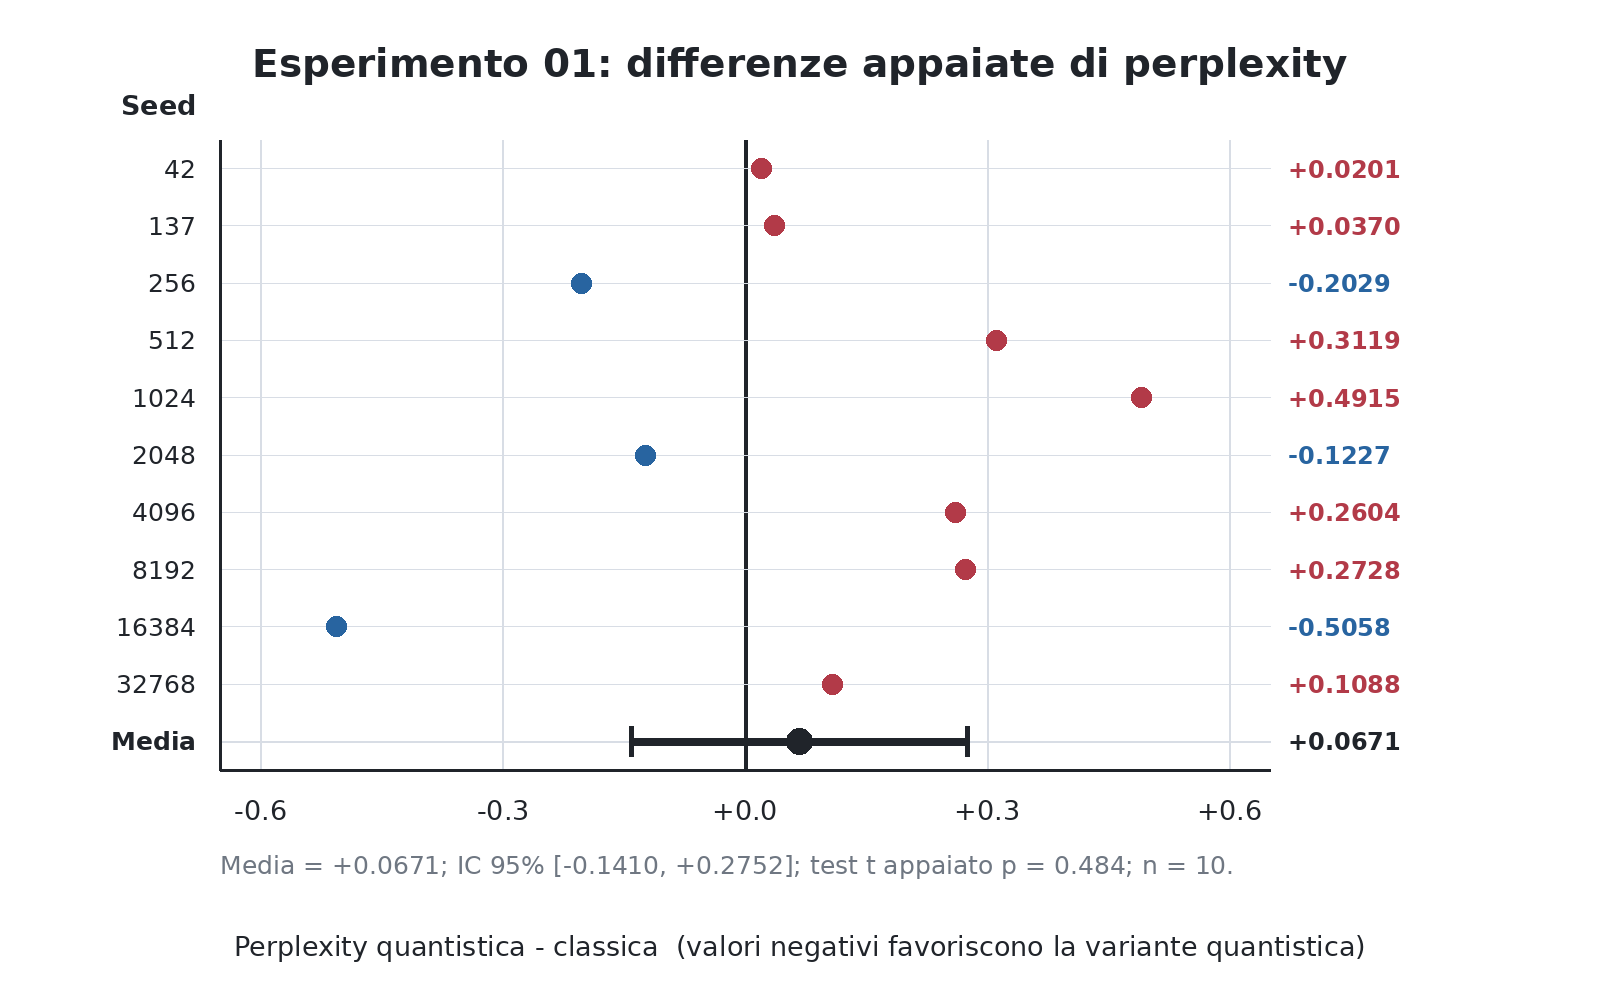
\includegraphics[width=.72\textwidth]{figure/experiment_01_paired_effects.png}
  \caption[Esperimento 01: differenze appaiate]{Differenza di perplexity
  quantistico meno classico per seed. Il punto finale è la media e la barra il
  relativo IC al 95\%.}
  \label{fig:paired-01}
\end{figure}

\subsection{Esperimento 02 --- \emph{Patch embedding} quantistico}

\begin{table}[htbp]
\centering
\caption[Esperimento 02: metriche di classificazione]{%
Esperimento~02, per dataset, 5 seed. Media $\pm$ deviazione standard.
\convsegno}
\label{tab:risultati-02}
\small
\begin{tabular}{@{}l l c c c c r@{}}
\toprule
\textbf{Dataset} & \textbf{Variante} & \textbf{Test acc.} & \textbf{macro-AUC} & \textbf{macro-F1} & $\gap$ & \textbf{Tempo (s)} \\
\midrule
\multirow{2}{*}{PathMNIST} & Classica    & $0{,}72232\pm0{,}02362$ & $0{,}95536\pm0{,}00436$ & $0{,}64840\pm0{,}03101$ & $0{,}01550\pm0{,}01710$ & $1124{,}5\pm38{,}1$ \\
                           & Quantistica & $0{,}69818\pm0{,}01830$ & $0{,}94520\pm0{,}00681$ & $0{,}63598\pm0{,}01843$ & $0{,}03384\pm0{,}02585$ & $10445{,}7\pm712{,}7$ \\
\bottomrule
\end{tabular}
\end{table}

L'accuracy quantistica meno classica è $-0{,}02414$ (IC $t$ al 95\%
$[-0{,}05432;+0{,}00604]$, $p=0{,}091$). L'IC bootstrap è interamente negativo,
ma la decisione primaria segue l'intervallo $t$. La macro-AUC diminuisce di
$0{,}01016$ (IC $[-0{,}01525;-0{,}00507]$, $p=0{,}005$) ed è inferiore in tutti
i cinque seed. La selezione dei checkpoint finali anziché best-validation non
cambia la conclusione. Le curve di apprendimento sono nella \cref{fig:curve-02}.

\begin{figure}[htbp]
\centering
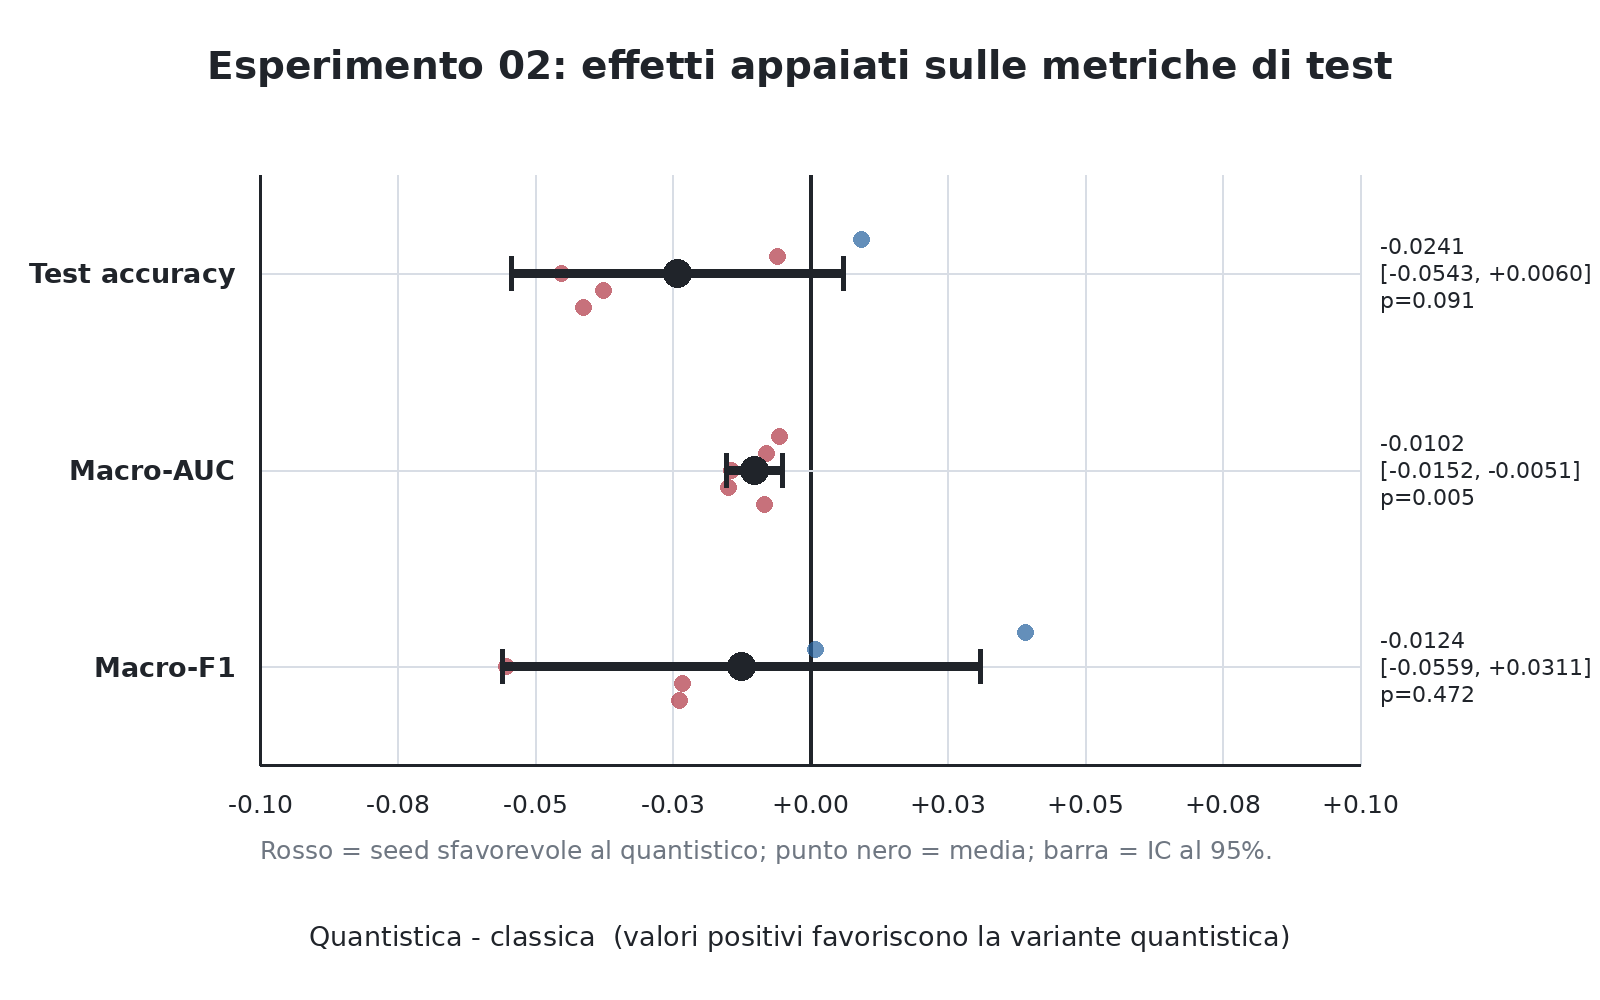
\includegraphics[width=.72\textwidth]{figure/experiment_02_paired_effects.png}
\caption[Esperimento 02: differenze appaiate]{Differenze quantistico meno
classico per le metriche di classificazione; barre: IC al 95\%.}
\label{fig:paired-02}
\end{figure}

\subsection{Esperimento 03 --- Ablazione sulla regolarizzazione}

È la tabella centrale della tesi.

\begin{table}[htbp]
\centering
\caption[Esperimento 03: tabella principale dell'ablazione]{%
Esperimento~03, per dataset e variante, 5 seed. Media $\pm$ deviazione standard.
Il gap $\gap = \acctr - \accte$ è la metrica primaria; $\acctr$ e $\accte$ sono
riportate accanto perché il gap è interpretabile solo a parità di accuracy di
training (\cref{sec:metriche}). \convsegno}
\label{tab:risultati-03}
\scriptsize
\begin{tabular}{@{}l l c c c c c r r@{}}
\toprule
\textbf{Dataset} & \textbf{Variante} & $\acctr$ & $\accte$ & $\gap$ & \textbf{AUC} & \textbf{F1} & \textbf{P.emb.} & \textbf{Tempo (s)} \\
\midrule
\multirow{3}{*}{PathMNIST}
 & \code{vanilla}      & $0{,}806\pm0{,}124$ & $0{,}448\pm0{,}027$ & $0{,}358\pm0{,}141$ & $0{,}768\pm0{,}026$ & $0{,}359\pm0{,}016$ & \num{1480} & $29{,}7\pm1{,}2$ \\
 & \code{bounded\_mlp} & $0{,}886\pm0{,}053$ & $0{,}464\pm0{,}029$ & $0{,}423\pm0{,}050$ & $0{,}754\pm0{,}020$ & $0{,}385\pm0{,}023$ & \num{1880} & $30{,}0\pm1{,}1$ \\
 & \code{quantum\_reg} & $0{,}950\pm0{,}050$ & $0{,}379\pm0{,}066$ & $0{,}571\pm0{,}096$ & $0{,}719\pm0{,}046$ & $0{,}322\pm0{,}055$ & \num{1540} & $1818{,}2\pm129{,}2$ \\
\midrule
\multirow{3}{*}{BloodMNIST}
 & \code{vanilla}      & $0{,}874\pm0{,}067$ & $0{,}565\pm0{,}039$ & $0{,}309\pm0{,}079$ & $0{,}845\pm0{,}027$ & $0{,}472\pm0{,}054$ & \num{1480} & $14{,}9\pm0{,}1$ \\
 & \code{bounded\_mlp} & $0{,}932\pm0{,}029$ & $0{,}536\pm0{,}051$ & $0{,}396\pm0{,}069$ & $0{,}819\pm0{,}035$ & $0{,}449\pm0{,}055$ & \num{1880} & $15{,}2\pm0{,}1$ \\
 & \code{quantum\_reg} & $0{,}916\pm0{,}139$ & $0{,}421\pm0{,}041$ & $0{,}495\pm0{,}157$ & $0{,}739\pm0{,}027$ & $0{,}348\pm0{,}046$ & \num{1540} & $961{,}5\pm26{,}0$ \\
\midrule
\multirow{3}{*}{DermaMNIST}
 & \code{vanilla}      & $0{,}772\pm0{,}104$ & $0{,}634\pm0{,}023$ & $0{,}138\pm0{,}125$ & $0{,}661\pm0{,}039$ & $0{,}158\pm0{,}041$ & \num{1480} & $13{,}8\pm0{,}1$ \\
 & \code{bounded\_mlp} & $0{,}770\pm0{,}105$ & $0{,}650\pm0{,}016$ & $0{,}120\pm0{,}117$ & $0{,}599\pm0{,}096$ & $0{,}159\pm0{,}042$ & \num{1880} & $14{,}0\pm0{,}1$ \\
 & \code{quantum\_reg} & $0{,}832\pm0{,}108$ & $0{,}628\pm0{,}041$ & $0{,}204\pm0{,}140$ & $0{,}607\pm0{,}035$ & $0{,}158\pm0{,}021$ & \num{1540} & $891{,}9\pm5{,}7$ \\
\bottomrule
\end{tabular}
\end{table}

\paragraph{Tracce diagnostiche.}
\begin{table}[htbp]
\centering
\caption[Esperimento 03: diagnostica su gradienti e attivazioni]{%
Norma $L^2$ media del gradiente in uscita da \code{patch\_embed.compression} e
frazione di attivazioni in saturazione (definita dalla \cref{eq:saturazione}),
mediate su epoche e seed. Il modulo osservato è identico nelle tre varianti.}
\label{tab:diagnostica-03}
\small
\begin{tabular}{@{}l c c@{}}
\toprule
\textbf{Variante} & \textbf{Norma media del gradiente} & \textbf{Frazione di saturazione} \\
\midrule
\code{vanilla}      & $0{,}198$ & $0{,}00113$ \\
\code{bounded\_mlp} & $0{,}185$ & $0{,}00049$ \\
\code{quantum\_reg} & $0{,}250$ & $0{,}00453$ \\
\bottomrule
\end{tabular}
\end{table}

Il delta di gap quantistico meno \code{bounded\_mlp} è $+0{,}148$ su
PathMNIST, $+0{,}100$ su BloodMNIST e $+0{,}085$ su DermaMNIST; il segno è
contrario a H3 in 12 blocchi dataset/seed su 15. Saturazione e gradienti non
indicano un collasso banale dell'ottimizzazione.

Il gap medio delle tre varianti, dataset per dataset, è rappresentato nella
\cref{fig:gap-03}.

\begin{figure}[htbp]
\centering
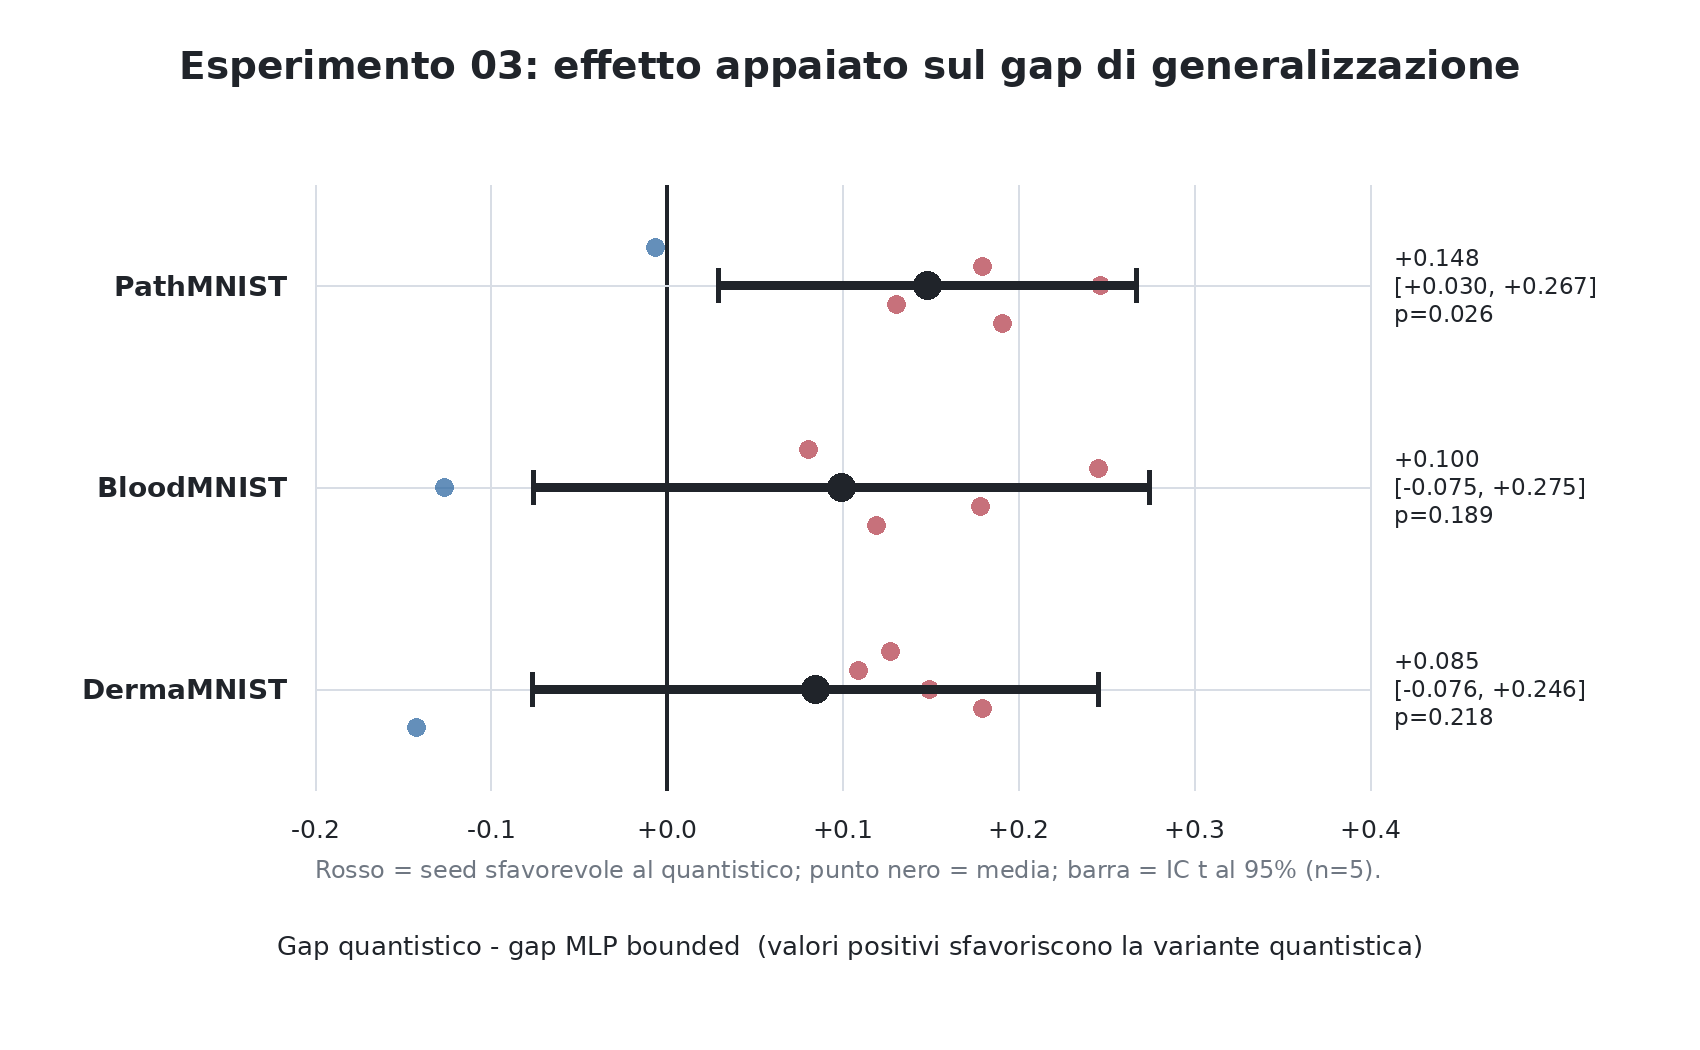
\includegraphics[width=.72\textwidth]{figure/experiment_03_paired_gap_effects.png}
\caption[Esperimento 03: differenze appaiate del gap]{Differenza di gap
\code{quantum\_reg} meno \code{bounded\_mlp} per dataset e seed. Valori
positivi sono contrari all'ipotesi di regolarizzazione; il punto aggregato
riporta media e IC al 95\%.}
\label{fig:paired-gap-03}
\end{figure}

\subsection{Esperimento 04 --- Kernel di fedeltà}

\begin{table}[htbp]
\centering
\caption[Esperimento 04: metriche di separabilità]{%
Esperimento~04, BreastMNIST, 80${+}$20 campioni, PCA a 8 componenti.
Media $\pm$ deviazione standard su 20 ripetizioni. Il criterio di Fisher è
la metrica primaria; il rapporto $\rho$ è descrittivo e non confrontabile fra
scale diverse (\cref{sec:metriche}). \convsegno}
\label{tab:risultati-04}
\small
\begin{tabular}{@{}l c c c c c@{}}
\toprule
\textbf{Kernel} & \code{intra\_0} & \code{intra\_1} & \code{inter} & $\rho$ & $F$ \\
\midrule
Coseno & $0{,}8922 \pm 0{,}0142$ & $0{,}8825 \pm 0{,}0158$ & $0{,}8816 \pm 0{,}0133$ & $1{,}0066 \pm 0{,}0043$ & $0{,}0180 \pm 0{,}0200$ \\
RBF & $0{,}6084 \pm 0{,}0108$ & $0{,}5473 \pm 0{,}0405$ & $0{,}5547 \pm 0{,}0210$ & $1{,}0424 \pm 0{,}0294$ & $0{,}0446 \pm 0{,}0513$ \\
Fedeltà (IQP) & $0{,}0172 \pm 0{,}0038$ & $0{,}0171 \pm 0{,}0067$ & $0{,}0145 \pm 0{,}0028$ & $1{,}1799 \pm 0{,}1451$ & $0{,}0029 \pm 0{,}0032$ \\
\bottomrule
\end{tabular}
\end{table}

Le otto componenti PCA spiegano $0{,}7654 \pm 0{,}0113$ della varianza
(intervallo osservato $[0{,}7459,0{,}7837]$). Sulla metrica primaria, la
differenza IQP meno coseno è $-0{,}01515$; IQP meno RBF è $-0{,}04168$. Il
rapporto $\rho$ ha invece segno opposto, come discusso nella
\cref{sec:limiti-statistici}: non sostituisce la metrica primaria dichiarata.

\begin{figure}[htbp]
\centering
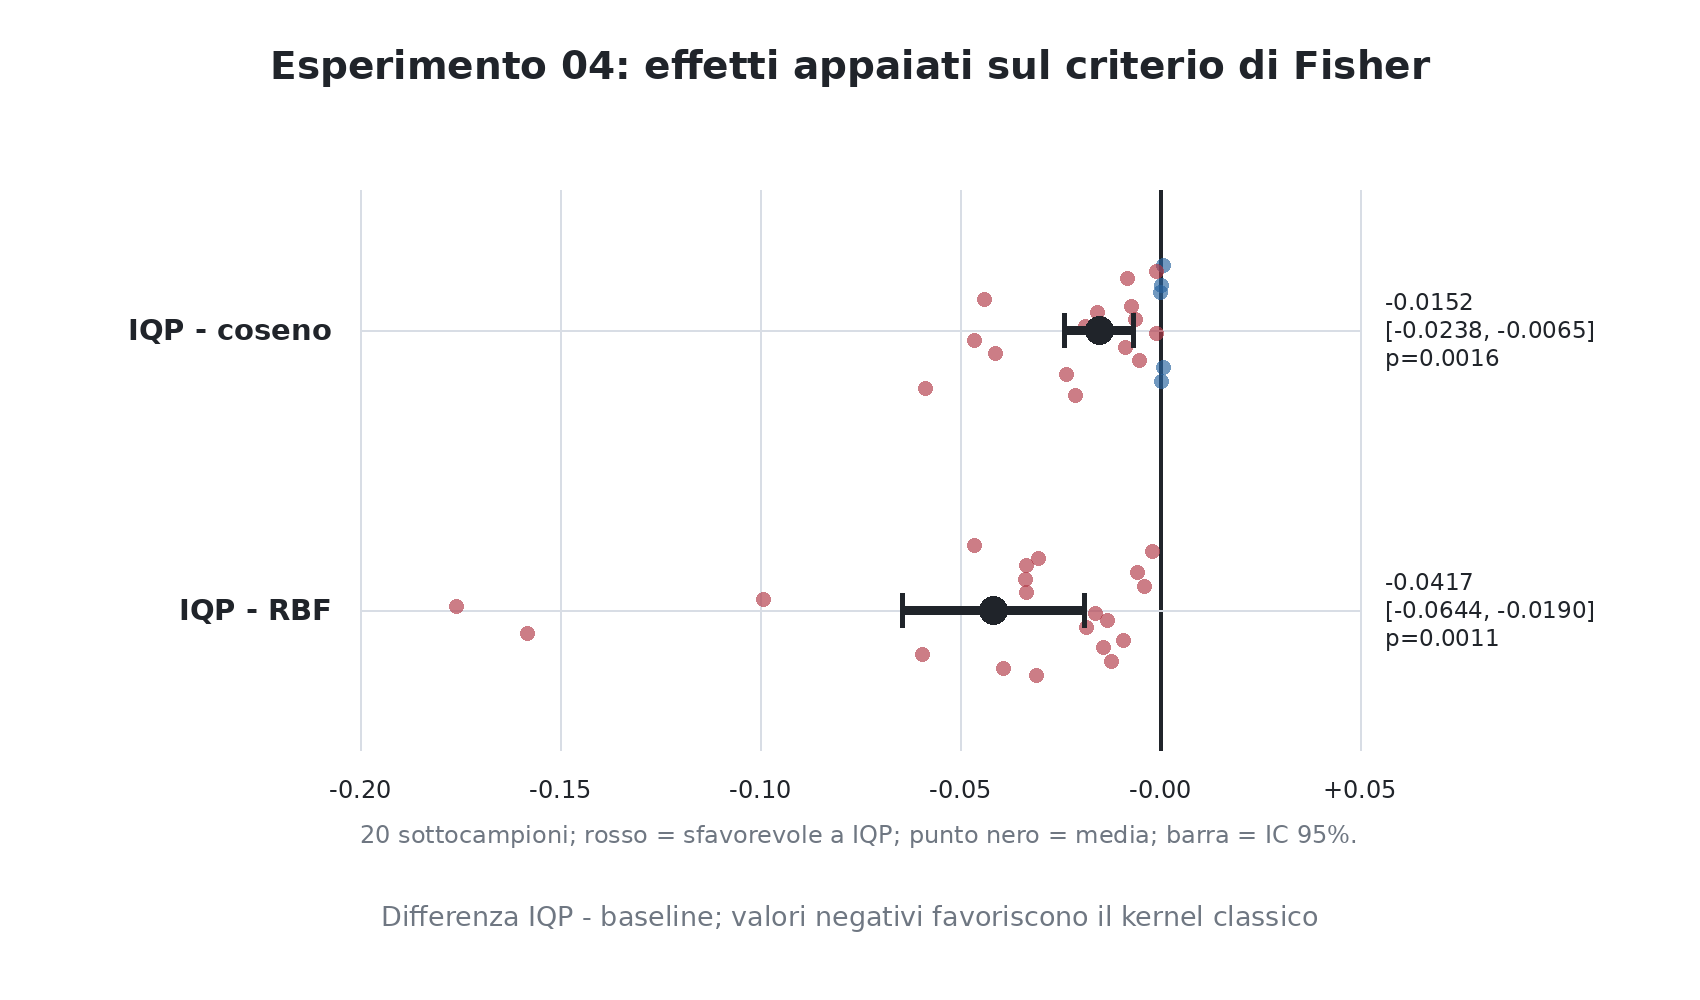
\includegraphics[width=.72\textwidth]{figure/experiment_04_fisher_effects.png}
\caption[Esperimento 04: effetti sul criterio di Fisher]{Differenze appaiate
IQP meno coseno e IQP meno RBF. Valori negativi indicano separabilità inferiore
del kernel quantistico; barre: IC al 95\%.}
\label{fig:fisher-04}
\end{figure}

La validazione predittiva fuori campione, con SVC a kernel precomputato sul test
ufficiale BreastMNIST e $C$ selezionato per cross-validation sui soli dati di
training, va nella stessa direzione della metrica primaria. IQP è inferiore a
coseno e RBF su balanced accuracy, macro-AUC e macro-F1 in tutti e tre i regimi di
composizione: nel regime 80/20 la balanced accuracy è $0{,}511$ contro $0{,}594$
del coseno, nel 50/50 $0{,}607$ contro $0{,}673$ e nel 27/73 $0{,}569$ contro
$0{,}688$. I valori completi sono nell'\cref{tab:validazione-svc-04}.

\begin{figure}[htbp]
\centering
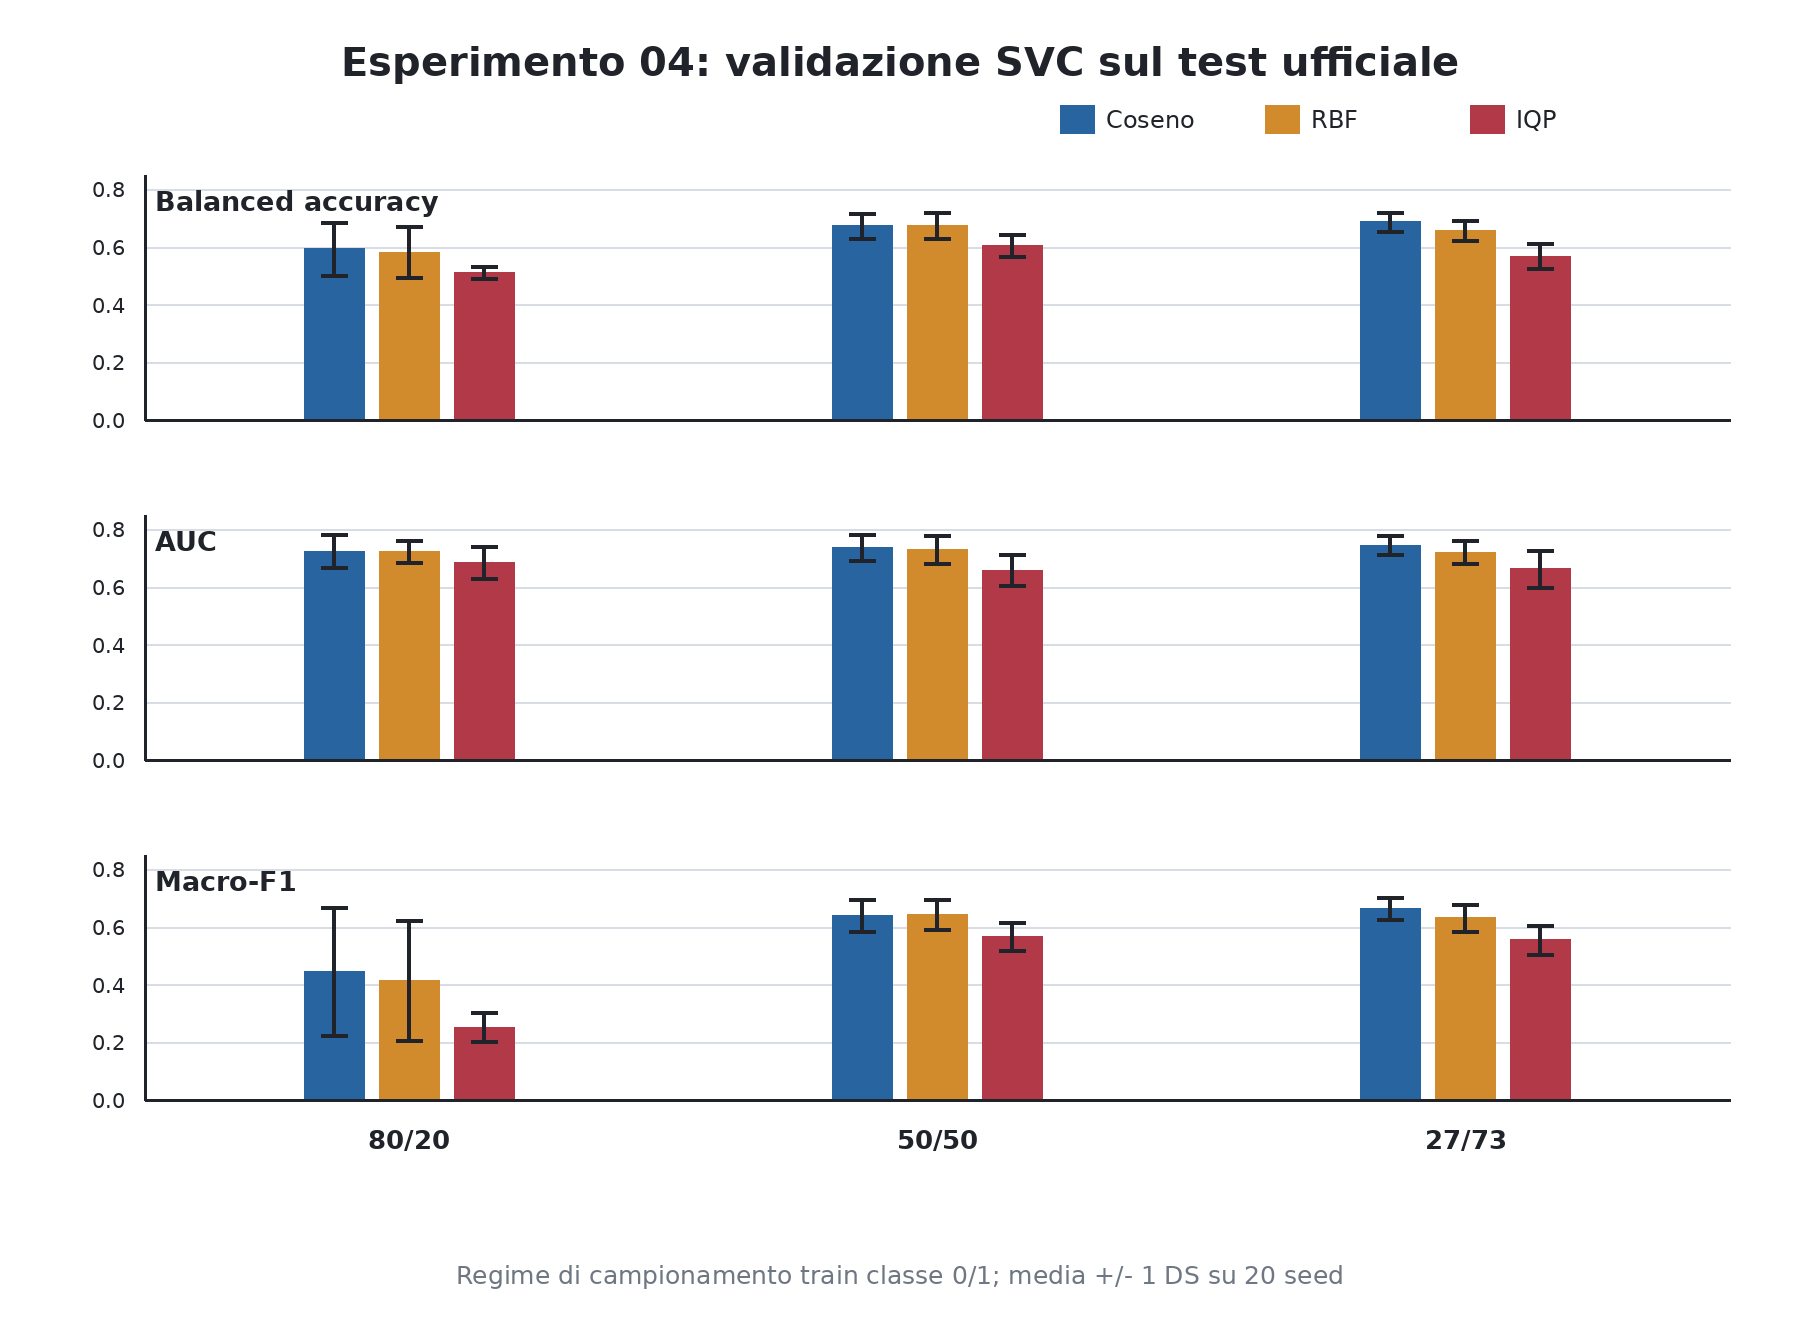
\includegraphics[width=.85\textwidth]{figure/experiment_04_svc_metrics.png}
\caption[Esperimento 04: metriche SVC]{Balanced accuracy, macro-AUC e macro-F1
della SVC con kernel precomputato nei regimi 80/20, 50/50 e 27/73. Le barre
riassumono la variabilità sui venti sottocampioni di training.}
\label{fig:svc-04}
\end{figure}

\section{Differenze appaiate}
\label{sec:differenze-appaiate}

Le differenze dell'esperimento 01 sono riportate nell'\cref{tab:seed-01}; le
figure \cref{fig:paired-01,fig:paired-02,fig:paired-gap-03,fig:fisher-04}
mostrano i punti appaiati, la media e l'intervallo. I valori aggregati sono
riuniti nella \cref{tab:statistica}.

Dove il segno della differenza non è consistente fra i seed, l'incoerenza è
riportata insieme al valore medio, perché descrive la stabilità del confronto.

\section{Intervalli di confidenza e dimensioni dell'effetto}
\label{sec:intervalli}

\begin{table}[htbp]
\centering
\caption[Analisi statistica dei confronti appaiati]{%
Analisi appaiata prodotta da \code{paired\_comparison()} sulle metriche primarie.
Sono riportati insieme differenza media, entrambi gli intervalli di confidenza, i
due valori $p$ e la dimensione dell'effetto: il valore $p$ da solo non è un
risultato (\cref{sec:statistica}). \convsegno}
\label{tab:statistica}
\scriptsize
\begin{tabular}{@{}l l c c c c c c@{}}
\toprule
\textbf{Confronto} & \textbf{Metrica} & $\dmean$ & $\IC$ ($t$) & $\IC$ (boot.) & $p_{t}$ & $p_{W}$ & $\dz$ \\
\midrule
04 IQP--coseno & Fisher & $-0{,}01515$ & $[-0{,}02379;-0{,}00652]$ & $[-0{,}02345;-0{,}00769]$ & $0{,}00161$ & $0{,}000322$ & $-0{,}821$ \\
04 IQP--RBF & Fisher & $-0{,}04168$ & $[-0{,}06438;-0{,}01899]$ & $[-0{,}06452;-0{,}02322]$ & $0{,}00109$ & $1{,}91\times10^{-6}$ & $-0{,}860$ \\
01 QGPT & PPL & $+0{,}06711$ & $[-0{,}14100;+0{,}27522]$ & $[-0{,}11048;+0{,}22839]$ & $0{,}484$ & $0{,}4316$ & $+0{,}231$ \\
02 QViT & Accuracy & $-0{,}02414$ & $[-0{,}05432;+0{,}00604]$ & $[-0{,}04208;-0{,}00386]$ & $0{,}0905$ & $0{,}1875$ & $-0{,}993$ \\
03 PathMNIST & Gap & $+0{,}14838$ & $[+0{,}030;+0{,}267]$ & $[+0{,}070;+0{,}212]$ & $0{,}026$ & $0{,}125$ & $+1{,}550$ \\
03 BloodMNIST & Gap & $+0{,}09954$ & $[-0{,}075;+0{,}275]$ & $[-0{,}024;+0{,}195]$ & $0{,}189$ & $0{,}3125$ & $+0{,}706$ \\
03 DermaMNIST & Gap & $+0{,}08462$ & $[-0{,}076;+0{,}246]$ & $[-0{,}034;+0{,}159]$ & $0{,}218$ & $0{,}3125$ & $+0{,}653$ \\
\bottomrule
\end{tabular}
\end{table}

Gli intervalli distinguono neutralità incerta per H1, stima sfavorevole ma IC
dell'accuracy attraversato da zero per H2, direzione media sfavorevole coerente
fra dataset per H3 e intervalli interamente opposti all'atteso per H4.

L'unica divergenza rilevante fra $t$-test, bootstrap e Wilcoxon riguarda
l'accuracy dell'esperimento 02, dove l'intervallo bootstrap è interamente negativo
mentre quello $t$ attraversa lo zero; la decisione primaria segue l'intervallo
$t$, come stabilito nella \cref{sec:statistica}. La dimensione dell'effetto è
interpretata con le soglie convenzionali di \textcite{cohen1988statistical}
($0{,}2$, $0{,}5$, $0{,}8$), che restano convenzioni, e va letta tenendo presente
il limite di rilevabilità $\dz \ge 1{,}68$ della \cref{ssec:potenza}.

Il conteggio dei parametri per componente e i tempi di esecuzione delle tre
campagne con addestramento sono nell'\cref{app:tabelle}. I rapporti temporali
restano separati per esperimento: una singola figura accuracy--tempo
suggerirebbe una frontiera comune fra workload non omogenei.

\section{Verifica delle ipotesi}
\label{sec:verifica-ipotesi}

\begin{table}[htbp]
\centering
\caption[Esito delle quattro ipotesi]{%
Esito delle quattro ipotesi della \cref{tab:ipotesi}. L'esito
\rifiutataopposta{} indica che l'intervallo di confidenza è interamente
collocato nella direzione contraria a quella attesa. \convsegno}
\label{tab:verifica-ipotesi}
\small
\begin{tabularx}{\textwidth}{@{}c X c c c c@{}}
\toprule
\textbf{\#} & \textbf{Metrica primaria} & $\dmean$ & $\IC$ & $p$ & \textbf{Esito} \\
\midrule
H1 & Perplexity di validation & $+0{,}06711$ & $[-0{,}14100;+0{,}27522]$ & $0{,}484$ & \rifiutata \\
H2 & Test accuracy & $-0{,}02414$ & $[-0{,}05432;+0{,}00604]$ & $0{,}091$ & \rifiutata \\
H3 & Gap (tre dataset) & $+0{,}148;+0{,}100;+0{,}085$ & vedi \cref{tab:statistica} & --- & \rifiutata \\
H4 & Criterio di Fisher & $-0{,}01515$ & $[-0{,}02379;-0{,}00652]$ & $0{,}00161$ & \rifiutataopposta \\
\bottomrule
\end{tabularx}
\end{table}

Dove l'ipotesi non è rifiutata, il dato risulta compatibile con l'assenza di
effetto senza dimostrare un'equivalenza, e l'ampiezza di effetto ancora
compatibile è quella delimitata dall'intervallo di confidenza riportato in
tabella. L'espressione «prestazioni equivalenti» non compare in questa tesi,
perché non sarebbe sostenibile senza una soglia di equivalenza fissata a priori
(\cref{sec:falsificazione}).

Le spiegazioni sono rimandate al \cref{cap:discussione}.

\chapter{Discussione}
\label{cap:discussione}

Il capitolo confronta i risultati con i meccanismi esaminati e separa le
spiegazioni sostenute dalle diagnostiche dalle ipotesi ancora da verificare.

\section{Compressione dimensionale}
\label{sec:compressione}

In tutti e tre gli esperimenti che lavorano su dati ad alta dimensione il
circuito quantistico opera \emph{dopo} una compressione severa, e la compressione
è realizzata da una trasformazione classica:

\begin{center}
\begin{tabular}{@{}l l r@{}}
\toprule
\textbf{Esperimento} & \textbf{Compressione} & \textbf{Fattore} \\
\midrule
01 & $\demb = 8 \to \nq = 4$ per testa, \code{nn.Linear} addestrabile & $2\times$ \\
03 & $\dpatch = 147 \to \dvit = 10$, \code{nn.Linear} addestrabile & $14{,}7\times$ \\
04 & $784 \to 8$, PCA non addestrabile & $98\times$ \\
\bottomrule
\end{tabular}
\end{center}

La trasformazione successiva al collo di bottiglia può usare soltanto
l'informazione conservata dalla compressione. I confronti valutano quindi il VQC
nelle dimensionalità indicate in tabella, non prima della riduzione.

Nell'esperimento~01 la differenza media di validation loss è $+0{,}00543$, con IC
al 95\% $[-0{,}01040;+0{,}02126]$. H1 non è supportata; l'intervallo non equivale
a un test di equivalenza.

Nell'esperimento~04 la PCA è fissa e comune ai kernel. Le otto componenti
conservano in media il $76{,}54\%$ della varianza totale, una misura che non
specifica quanta parte della struttura discriminante rimanga nello spazio
compresso.

La dipendenza dalla compressione richiede confronti a dimensionalità diverse,
per esempio $\dvit \in \{4,10,16,32\}$ (\cref{sec:sviluppi}).

\section{Codifica angolare e saturazione}
\label{sec:saturazione}

La codifica angolare limita gli ingressi a $[-\pi,\pi]$ mediante una $\tanh$
(\cref{sec:quantum-linear}). Per $\abs{x}$ grande, la derivata tende a zero e
attenua il gradiente diretto allo strato di compressione.

Gli \emph{hook} dell'esperimento~03 registrano a ogni epoca saturazione e norma
media del gradiente (\cref{tab:diagnostica-03}). La saturazione media resta sotto
$0{,}013$ in ogni combinazione di dataset e variante. La norma del gradiente nel
modulo di compressione quantistico supera quella di \code{bounded\_mlp} nei tre
dataset. Le misure non indicano saturazione diffusa o gradienti più piccoli nel
modulo osservato, ma non coprono i parametri del circuito.

La connessione residua somma un ramo identità non limitato all'uscita del VQC,
confinata in $[-1,1]$. Un rapporto crescente fra le norme dei due rami
ridurrebbe il contributo relativo del circuito, ma gli \emph{hook} non registrano
questa quantità.

I \emph{barren plateau} riguardano la concentrazione dei gradienti nei circuiti
variazionali \parencite{mcclean2018barren}. Gli esperimenti usano 4--10 qubit e
due strati, senza misurare la varianza dei gradienti al variare di scala e
profondità. Le diagnostiche disponibili non verificano questo fenomeno.

\section{Capacità e sotto-adattamento}
\label{sec:capacita}

Il gap va letto insieme all'accuracy di training: può aumentare sia quando il
modello adatta meglio il training senza trasferire il guadagno al test, sia
quando cambiano entrambe le accuracy.

L'accuracy di training di \code{quantum\_reg} contro
\code{bounded\_mlp} è $0{,}950$ contro $0{,}886$ su PathMNIST, $0{,}916$ contro
$0{,}932$ su BloodMNIST e $0{,}832$ contro $0{,}770$ su DermaMNIST. Su PathMNIST e
DermaMNIST la variante quantistica adatta il training più strettamente della
baseline e ottiene un'accuracy di test inferiore; su BloodMNIST l'accuracy di
training è simile e quella di test resta inferiore. Il risultato non corrisponde
a un sotto-adattamento sistematico.

Il conteggio dei parametri non distingue una capacità effettiva ridotta da una
funzione difficile da ottimizzare. Curve ferme su un plateau basso favorirebbero
la prima spiegazione; curve ancora in salita o gradienti sistematicamente piccoli
la seconda. Le tracce raccolte non mostrano una delle due firme in modo stabile.

In nessuno dei tre dataset \code{quantum\_reg} riduce il gap rispetto a
\code{bounded\_mlp}; H3 non trova riscontro nella configurazione esaminata.

\section{Overhead di simulazione}
\label{sec:overhead}

Il rapporto fra i tempi della variante quantistica e di quella classica è
$46{,}5\times$ nell'esperimento 01, $9{,}29\times$ nel 02 e compreso fra
$60{,}7\times$ e $63{,}5\times$ nel 03; per il kernel dell'esperimento 04 il costo
è dominato dal calcolo quadratico delle similarità IQP. Il costo osservato dipende
dal backend a vettore di stato, dalla valutazione del QNode riga per riga
(\cref{sec:integrazione}), dal numero di qubit, dalla retropropagazione attraverso
le porte simulate e, nell'esperimento~01, dai
$n_{\text{layer}} \times \nhead \times 3$ circuiti valutati a ogni
\emph{forward pass}.

Il costo di simulazione ha imposto modelli piccoli, 4--10 qubit, cinque seed
negli esperimenti 02--03 e cento campioni nell'esperimento~04. I rapporti
temporali riguardano il simulatore e non l'esecuzione su hardware
(\cref{sec:costo}).

\section{Equità delle baseline}
\label{sec:equita-baseline}

Il conteggio dei parametri controlla solo una parte del confronto. La baseline
dell'esperimento~03 ha \num{1880} parametri di
\emph{patch embedding} contro \num{1540} della variante quantistica e ne replica
la limitatezza dell'output, mentre nell'esperimento~02 è la variante quantistica
ad averne 48 in più. Il numero di parametri non misura direttamente la capacità
delle due famiglie funzionali.

Learning rate, weight decay, numero di epoche e scheduler sono comuni e sono
stati fissati sulla baseline classica. Un tuning separato, con lo stesso budget
per ciascuna variante, rimane da eseguire (\cref{sec:sviluppi}).

Negli esperimenti 01 e 02 l'adapter classico addestrabile posto prima del
circuito rende l'effetto misurato quello della
composizione adapter${}+{}$VQC (\cref{sec:adapter}). L'esperimento~03 non usa
questo adapter. Nell'esperimento~04, IQP è confrontato con il coseno e con un RBF
a bandwidth mediana; non sono state provate altre famiglie di kernel o strategie
di selezione degli iperparametri.

\section{Limiti statistici}
\label{sec:limiti-statistici}

Il limite principale è la numerosità. Con cinque seed negli esperimenti 02 e 03 la
dimensione dell'effetto minima rilevabile con potenza $0{,}8$ è $\dz = 1{,}68$, e
con i dieci seed dell'esperimento 01 scende a circa $1{,}00$
(\cref{ssec:potenza}). Effetti moderati potevano quindi non essere rilevati. I
venti sottocampioni dell'esperimento~04 si sovrappongono e condividono il test
ufficiale nella validazione SVC; non sono venti dataset indipendenti.

Nell'esperimento~04 IQP aumenta $\rho$ rispetto al coseno ma riduce il criterio
di Fisher. $\rho$ dipende dalla scala e dal livello medio delle similarità; le
metriche della SVC forniscono il controllo predittivo. Balanced accuracy, AUC e
macro-F1 sono inferiori per IQP nei tre regimi di campionamento.

Non è stata definita una soglia di equivalenza né applicata una correzione per le
quattro ipotesi. L'analisi inferenziale riguarda le metriche primarie indicate
nel protocollo.

Nell'esperimento 01 la deviazione standard delle differenze di loss è
$0{,}02213$, contro una media di $0{,}00543$; nell'esperimento 02 la deviazione
delle differenze di accuracy è $0{,}0243$, contro una media in valore assoluto di
$0{,}0241$. Il segno della differenza varia quindi fra seed.

\section{Portata dei risultati negativi}
\label{sec:portata}

Le condizioni testate sono quelle riassunte nella \cref{sec:minacce}: codifica
angolare e ansatz \code{StronglyEntanglingLayers}, da 4 a 10 qubit e 2 strati
variazionali, in due sole posizioni architetturali, su MedMNIST a $28\times28$ e
su un corpus a livello di caratteri, con baseline appaiate e cinque o dieci seed.

In queste condizioni non emerge il miglioramento atteso della validation loss (H1) o
dell'accuracy di classificazione (H2); la macro-AUC di H2 è inferiore. Il gap di
generalizzazione non diminuisce ed è mediamente maggiore nei tre dataset di H3.
Per H4, il kernel di fedeltà IQP a 8 qubit ottiene valori inferiori al coseno e
all'RBF sia sul criterio di Fisher sia nella classificazione fuori campione.

Non sono stati esaminati altri ansatz, codifiche apprese, \emph{amplitude
embedding}, \emph{data re-uploading}, circuiti più grandi, altri domini o
hardware quantistico. Il lavoro non valuta vantaggi computazionali, cioè
l'affermazione (a) della \cref{ssec:quattro-promesse}.

I risultati riguardano le quattro configurazioni descritte. La variazione fra
seed rende instabile il segno delle differenze piccole.

L'infrastruttura comprende appaiamento dei seed, verifica dei componenti
condivisi, corruzioni deterministiche, manifest di provenienza e schema dei
risultati versionato. Può essere riutilizzata per altre configurazioni.

\chapter{Conclusioni}
\label{cap:conclusioni}

\section{Risposte alle domande di ricerca}
\label{sec:risposte}

\paragraph{H1 --- Proiezioni \texorpdfstring{$Q,K,V$}{Q,K,V} quantistiche.}
H1 è \nonsupportata. La differenza media di validation loss, quantistico meno
classico, è $+0{,}00543$ (IC al 95\% $[-0{,}01040;+0{,}02126]$, $p=0{,}458$).

\paragraph{H2 --- \emph{Patch embedding} quantistico.}
H2 è \nonsupportata. L'accuracy diminuisce in media di $0{,}02414$ (IC al 95\%
$[-0{,}05432;+0{,}00604]$, $p=0{,}091$). La macro-AUC è inferiore nei cinque seed
($-0{,}01016$, IC $[-0{,}01525;-0{,}00507]$).

\paragraph{H3 --- Regolarizzazione implicita.}
H3 è \nonsupportata. Il delta di gap quantistico meno \code{bounded\_mlp} è
positivo su PathMNIST ($+0{,}148$), BloodMNIST ($+0{,}100$) e DermaMNIST
($+0{,}085$), con segno positivo in 12 delle 15 coppie dataset/seed. Solo
l'intervallo di PathMNIST è interamente positivo.

\paragraph{H4 --- Kernel di fedeltà.}
Per H4 emerge \evidenzacontraria. Rispetto al coseno, la differenza media del
criterio di Fisher è $-0{,}01515$ (IC al 95\% $[-0{,}02379;-0{,}00652]$); rispetto all'RBF
è $-0{,}04168$ (IC $[-0{,}06438;-0{,}01899]$). La validazione SVC sul test
ufficiale produce metriche inferiori per IQP nei tre regimi di campionamento.

\paragraph{Risposta alla domanda generale.} Nessuno dei quattro esperimenti
mostra il vantaggio ipotizzato nelle configurazioni provate. La tesi valuta le
accezioni (b), (c) e (d) della \cref{ssec:quattro-promesse}; non misura uno
speedup computazionale.

\section{Contributi}
\label{sec:contributi-finali}

Il lavoro comprende quattro esperimenti appaiati e il pacchetto
\code{quantum\_framework}, che raccoglie layer PyTorch--PennyLane, caricamento dei
dati, addestramento, diagnostiche e analisi statistica. Configurazioni, seed,
comandi e tabelle complete sono conservati con uno schema dei risultati
versionato. La procedura di riproduzione è nell'appendice~\ref{app:riproduzione}.

\section{Limiti}
\label{sec:limiti}

I circuiti hanno 4--10 qubit, due strati, un solo ansatz e una sola codifica. I
VQC sostituiscono componenti circoscritti di modelli altrimenti classici, su
MedMNIST a $28\times28$ e su un corpus a caratteri. Gli esperimenti 02--03 usano
cinque seed, corrispondenti a un $\dz$ minimo rilevabile di $1{,}68$
(\cref{ssec:potenza}). Gli iperparametri sono stati scelti sulla baseline
classica; negli esperimenti 01--02 viene misurata la composizione
adapter${}+{}$VQC. Tutte le esecuzioni quantistiche sono simulate. Il costo della
simulazione ha determinato la scala dei modelli e dei campioni
(\cref{sec:overhead}).

\section{Sviluppi successivi}
\label{sec:sviluppi}

\begin{enumerate}
  \item Variare la dimensionalità compressa per misurare la dipendenza dal collo
    di bottiglia.
  \item Provare altre codifiche, profondità e ansatz, inclusi \emph{data
    re-uploading} e kernel addestrabili.
  \item Aumentare i seed e definire prima dell'esperimento una soglia di
    equivalenza per un TOST. Con 10 e 20 coppie, il $\dz$ minimo rilevabile
    stimato scende rispettivamente a $1{,}00$ e $0{,}66$.
  \item Selezionare separatamente gli iperparametri delle due varianti con lo
    stesso budget; per l'esperimento~04 questo include la bandwidth dell'RBF.
  \item Eseguire un sottoinsieme su hardware per misurare rumore di
    campionamento, costo dei gradienti e tempi.
\end{enumerate}


% ------------------------------------------------------------- APPENDICI ---
\appendix
% ===========================================================================
%  Appendice A — Configurazioni complete
% ===========================================================================
\chapter{Configurazioni complete}
\label{app:configurazioni}

Questa appendice riporta in forma tabellare il contenuto dei file
\file{config.json} salvati dalle run utilizzate nella tesi. Ogni
\file{config.json} è autodescrittivo: include sia i campi della dataclass sia le
proprietà calcolate (\cref{sec:base-config}), e può quindi essere interpretato
senza reistanziare il codice.

\section{Esperimento 01 --- preset di \texorpdfstring{\classe{GPTConfig}}{GPTConfig}}

\begin{table}[htbp]
\centering
\caption[Preset di configurazione dell'esperimento 01]{%
Preset disponibili in \file{01\_quantum\_gpt/src/config/}. Il valore di $\nq$ è
calcolato come $\demb/\nhead$ e non è un campo indipendente. Il preset
\code{big} non è utilizzabile nella variante quantistica: 64 qubit non sono
simulabili.}
\label{tab:preset-gpt}
\small
\begin{tabular}{@{}l r r r r r r r c@{}}
\toprule
\textbf{Preset} & $\demb$ & $\nhead$ & $n_{\text{layer}}$ & $\nq$ & \code{block\_size} & \code{max\_iters} & \code{lr} & \code{use\_quantum} \\
\midrule
\code{default} & 32  & 8  & 4 & 4  & 64  & \num{5000}  & \num{1e-3} & \code{False} \\
\code{fast}    & 8   & 2  & 2 & 4  & 8   & 500         & \num{3e-3} & \code{True} \\
\code{thesis}  & 8   & 2  & 2 & 4  & 16  & \num{1500}  & \num{3e-3} & \code{False} \\
\code{light}   & 32  & 4  & 2 & 8  & 16  & \num{1000}  & \num{1e-3} & \code{False} \\
\code{heavy}   & 128 & 32 & 9 & 4  & 128 & \num{20000} & \num{3e-4} & \code{False} \\
\code{big}     & 384 & 6  & 6 & 64 & 256 & \num{20000} & \num{3e-4} & \code{False} \\
\bottomrule
\end{tabular}
\end{table}

La campagna definitiva usa il preset \code{thesis}, riportato per esteso qui
sotto; le due varianti differiscono soltanto nel campo \code{use\_quantum}.

\begin{center}
\begin{tabular}{@{}l l l l@{}}
\toprule
\textbf{Campo} & \textbf{Valore} & \textbf{Campo} & \textbf{Valore} \\
\midrule
\code{tokenizer\_class} & \code{CharTokenizer} & \code{batch\_size} & 8 \\
\code{block\_size} & 16 & \code{max\_iters} & 1500 \\
\code{eval\_interval} & 100 & \code{eval\_iters} & 100 \\
\code{learning\_rate} & \num{3e-3} & \code{dropout} & 0 \\
\code{n\_embd} & 8 & \code{n\_head} & 2 \\
\code{n\_layer} & 2 & \code{n\_qubits} & 4 \\
\code{n\_qlayers} & 2 & \code{q\_device} & \code{default.qubit} \\
\code{device} & \code{cpu} & \code{use\_quantum} & \code{False}/\code{True} \\
\bottomrule
\end{tabular}
\end{center}

\section{Esperimento 02 --- \texorpdfstring{\classe{QViTConfig}}{QViTConfig}}

\begin{center}\small
\begin{tabular}{@{}l l l l@{}}\toprule
\textbf{Campo}&\textbf{Valore}&\textbf{Campo}&\textbf{Valore}\\\midrule
\code{dataset}&\code{pathmnist}&\code{max\_epochs}&50\\
\code{embed\_dim}&8&\code{n\_head}&2\\
\code{n\_layer}&2&\code{ffn\_dim}&32\\
\code{patch\_size}&7&\code{batch\_size}&128\\
\code{dropout}&0,1&\code{weight\_decay}&\num{1e-4}\\
\code{n\_qlayers}&2&\code{q\_device}&\code{default.qubit}\\
\code{device}&\code{cpu}&\code{use\_quantum}&\code{False}/\code{True}\\\bottomrule
\end{tabular}\end{center}

\section{Esperimento 03 --- \texorpdfstring{\classe{AblationConfig}}{AblationConfig}}

\begin{center}\small
\begin{tabular}{@{}l l l l@{}}\toprule
\textbf{Campo}&\textbf{Valore}&\textbf{Campo}&\textbf{Valore}\\\midrule
\code{datasets}&Path/Blood/Derma&\code{train\_subset}&100\\
\code{optimizer\_steps}&400&\code{eval\_interval}&40\\
\code{embed\_dim}&10&\code{n\_head}&2\\
\code{n\_layer}&2&\code{ffn\_dim}&40\\
\code{patch\_size}&7&\code{batch\_size}&128\\
\code{dropout}&0&\code{weight\_decay}&0\\
\code{n\_qlayers}&2&\code{q\_device}&\code{default.qubit}\\
\code{device}&\code{cuda}&\code{evaluate\_noise}&\code{False}\\\bottomrule
\end{tabular}\end{center}
Le varianti sono \code{vanilla}, \code{bounded\_mlp} e
\code{quantum\_reg}; canali e classi sono determinati dal dataset.

\section{Esperimento 04 --- argomenti della riga di comando}

L'esperimento~04 non usa una dataclass di configurazione: i suoi parametri sono
argomenti della CLI, registrati nel campo \code{command} di
\file{run\_manifest.json} e replicati nei campi di primo livello di
\file{results.json} (\code{dataset}, \code{seed}, \code{n\_qubits},
\code{n\_class0}, \code{n\_class1}, \code{q\_device}).

\chapter{Ambiente e comandi di riproduzione}
\label{app:riproduzione}

\section{Struttura del repository}

\begin{lstlisting}[style=shell, numbers=none]
quantum-ml-research/
|-- run.py                      # entry point comune ai quattro esperimenti
|-- pyproject.toml              # manifest unico delle dipendenze (uv)
|-- uv.lock                     # ambiente pinnato, autoritativo
|
|-- quantum_framework/          # libreria condivisa, installata come package
|   |-- layers/quantum_linear.py
|   |-- data/medmnist_loader.py
|   |-- training/trainer.py
|   |-- evaluation/{metrics.py, statistics.py}
|   `-- utils/{config.py, experiment.py}
|
|-- experiments/
|   |-- 01_quantum_gpt/         # proiezioni Q,K,V quantistiche
|   |-- 02_quantum_vit/         # patch embedding quantistico
|   |-- 03_quantum_reg/         # ablazione sulla regolarizzazione
|   `-- 04_quantum_kernel/      # kernel di fedelta vs similarita coseno
|
|-- tests/                      # test_config.py, test_metrics.py, test_statistics.py
`-- docs/
\end{lstlisting}

\section{Installazione}

\begin{lstlisting}[style=shell, numbers=none]
git clone <url-del-repository>
cd quantum-ml-research
uv sync               # dipendenze principali (esperimenti 02, 03, 04)
uv sync --extra gpt   # aggiunge torchinfo, torchviz, datasets, transformers (esp. 01)
uv sync --extra gpu   # aggiunge pennylane-lightning[gpu]
\end{lstlisting}

L'ambiente pinnato è \file{uv.lock} ed è la fonte autoritativa;
\file{requirements.txt} è un riassunto leggibile e non va usato per installare.
Per la simulazione accelerata su GPU, oltre all'extra \code{gpu}, occorre
impostare \code{q\_device = "lightning.qubit"} nella configurazione al posto di
\code{default.qubit}.

\section{Controlli preliminari}

Prima dell'esecuzione si controllano albero di lavoro e test:

\begin{lstlisting}[style=shell, numbers=none]
git status --porcelain                                  # deve essere vuoto
uv run python -m unittest discover -s tests -v
uv run pre-commit run --all-files                       # ruff: lint e formattazione
\end{lstlisting}

Prima di una run completa si esegue inoltre uno \emph{smoke test} con poche
epoche, controllando forme dei tensori, checkpoint e schema delle metriche.

\section{Invarianti di configurazione}
\label{app:invarianti}

Il metodo \code{\_\_post\_init\_\_} di \classe{BaseViTConfig}
(\cref{sec:base-config}) verifica $H \bmod p = 0$,
$\dvit \bmod \nhead = 0$ e la positività di dimensioni e profondità. In caso di
violazione solleva \code{ValueError} prima di costruire il modello.

\section{Valutazione di robustezza al rumore}
\label{ssec:rumore}

Il metodo \code{\_test\_noise\_robustness()} di \classe{BaseTrainer} valuta il
modello addestrato su due tipi di corruzione, rumore gaussiano e \emph{sale e
pepe}, a cinque intensità $\{0{,}05,\ 0{,}1,\ 0{,}2,\ 0{,}3,\ 0{,}5\}$, riportando
loss, accuracy, AUC e F1 per ogni combinazione. Il seed delle corruzioni è
derivato in modo deterministico da quello della run, secondo
\code{seed + 10000 + indice\_tipo·100 + indice\_intensità}.

Le varianti con lo stesso seed ricevono le stesse corruzioni. La run definitiva
dell'esperimento~03 non include questa valutazione.

\section{Esperimento 01 --- Quantum GPT}

\begin{lstlisting}[style=shell, numbers=none]
uv run python run.py 01 --mode compare --config thesis \
  --dataset data/input.txt \
  --seeds 42,137,256,512,1024,2048,4096,8192,16384,32768 \
  --name thesis_shakespeare --force_cpu --resume
\end{lstlisting}

Corpus, preset e seed devono restare invariati fra le due varianti. L'aggregato
è scritto in \file{experiments/comparison\_thesis\_shakespeare.json}; la copia
congelata è \file{docs/checkpoints/experiment\_01\_quantum\_gpt\_n10.json}.

\section{Esperimento 02 --- Quantum ViT}

\begin{lstlisting}[style=shell, numbers=none]
uv run python run.py 02 compare --dataset pathmnist --epochs 50 \
  --seeds 42 137 256 512 1024 --name thesis_pathmnist \
  --q-device default.qubit --force-cpu
\end{lstlisting}

In caso di interruzione si ripete lo stesso comando aggiungendo \code{--resume}:
il checkpoint atomico conserva modello, ottimizzatore, scheduler, storico, RNG e
stato del generatore del DataLoader. PathMNIST è il test primario; le eventuali
repliche su altri dataset sono analisi secondarie e mantengono invariati gli
iperparametri fra le varianti.

\section{Esperimento 03 --- Ablazione sulla regolarizzazione}

\begin{lstlisting}[style=shell, numbers=none]
uv run python run.py 03 ablation --epochs 400 --train-subset 100 \
  --seeds 42 137 256 512 1024 \
  --datasets pathmnist bloodmnist dermamnist \
  --dropout 0 --weight-decay 0 --eval-interval 40 --skip-noise
\end{lstlisting}

La run comprende $3 \times 5 \times 3 = 45$ run e salva
\file{ablation\_progress.json} dopo ciascuna. In caso di interruzione:

\begin{lstlisting}[style=shell, numbers=none]
uv run python run.py 03 ablation --epochs 400 --train-subset 100 \
  --dropout 0 --weight-decay 0 --eval-interval 40 --skip-noise \
  --resume experiments/ablation_thesis_regularization.progress.json
\end{lstlisting}

\section{Esperimento 04 --- Kernel quantistico}

\begin{lstlisting}[style=shell, numbers=none]
uv run python run.py 04 --seed 42 --repeats 1 \
  --n-class0 80 --n-class1 20 --n-qubits 8 \
  --feature-map iqp --iqp-repeats 2 --kernel-method statevector
uv run python run.py 04 --seed 42 --repeats 20 \
  --n-class0 80 --n-class1 20 --n-qubits 8 \
  --feature-map iqp --iqp-repeats 2 --kernel-method pairwise
\end{lstlisting}

Ogni ripetizione usa il seed $\code{seed} + r$ e salva gli indici selezionati e
la varianza spiegata dalla PCA, oltre alle matrici dei kernel. I controlli di
separabilità usano il metodo a vettore di stato:

\begin{lstlisting}[style=shell, numbers=none]
uv run python run.py 04 --seed 42 --repeats 20 \
  --n-class0 50 --n-class1 50 --n-qubits 8 \
  --feature-map iqp --iqp-repeats 2 --kernel-method statevector
uv run python run.py 04 --seed 42 --repeats 20 \
  --n-class0 27 --n-class1 73 --n-qubits 8 \
  --feature-map iqp --iqp-repeats 2 --kernel-method statevector
\end{lstlisting}

La validazione SVC è eseguita dalla directory
\file{experiments/04\_quantum\_kernel} nei regimi 80/20, 50/50 e 27/73:

\begin{lstlisting}[style=shell, numbers=none]
uv run python classifier_validation.py --n-class0 80 --n-class1 20 \
  --repeats 20 --seed 42
uv run python classifier_validation.py --n-class0 50 --n-class1 50 \
  --repeats 20 --seed 42
uv run python classifier_validation.py --n-class0 27 --n-class1 73 \
  --repeats 20 --seed 42
\end{lstlisting}

\section{Output di una run}

Ogni esecuzione scrive in una directory identificata da un timestamp:

\begin{itemize}
  \item \file{config.json} --- snapshot completo della configurazione, comprensivo
    delle proprietà calcolate;
  \item \file{run\_manifest.json} --- provenienza: commit, flag \emph{dirty},
    riga di comando, timestamp, versioni di librerie e hardware;
  \item \file{params.json} --- conteggio dei parametri per componente
    (esperimenti 02 e 03);
  \item \file{best\_model.pth} e \file{final\_model.pth} --- checkpoint
    selezionato sulla validation e stato dell'ultima epoca;
  \item \file{results.json} --- metriche, gap, storia per epoca ed eventuale
    robustezza al rumore;
  \item \file{events.out.tfevents.*} --- log TensorBoard.
\end{itemize}

\section{Controlli prima dell'analisi}

Prima dell'analisi si verificano completezza delle coppie, seed, configurazioni e
valori finiti nei \file{results.json}. Le tabelle derivano dagli aggregati JSON.

\chapter{Tabelle complete}
\label{app:tabelle}

Il \cref{cap:risultati} riporta gli aggregati; qui sono raccolti i valori per
singola run e le tabelle di supporto.

\section{Risultati per seed}

\begin{longtable}{@{}r r r r r r@{}}
\caption{Esperimento 01: risultati completi per seed. I delta sono definiti
come quantistico meno classico.}\label{tab:seed-01}\\
\toprule
\textbf{Seed} & $\mathcal{L}_c$ & $\mathcal{L}_q$ & $\Delta\mathcal{L}$ & $\PPL_c$ & $\PPL_q$ \\
\midrule
\endfirsthead
\toprule
\textbf{Seed} & $\mathcal{L}_c$ & $\mathcal{L}_q$ & $\Delta\mathcal{L}$ & $\PPL_c$ & $\PPL_q$ \\
\midrule
\endhead
42    & 2,5370 & 2,5385 & +0,0015 & 12,6411 & 12,6612 \\
137   & 2,5708 & 2,5736 & +0,0028 & 13,0764 & 13,1134 \\
256   & 2,5570 & 2,5411 & -0,0159 & 12,8971 & 12,6942 \\
512   & 2,5671 & 2,5908 & +0,0237 & 13,0282 & 13,3401 \\
1024  & 2,5251 & 2,5637 & +0,0386 & 12,4917 & 12,9832 \\
2048  & 2,5758 & 2,5665 & -0,0093 & 13,1423 & 13,0196 \\
4096  & 2,5697 & 2,5894 & +0,0197 & 13,0615 & 13,3219 \\
8192  & 2,5184 & 2,5401 & +0,0217 & 12,4084 & 12,6812 \\
16384 & 2,6341 & 2,5971 & -0,0370 & 13,9303 & 13,4245 \\
32768 & 2,5464 & 2,5549 & +0,0085 & 12,7612 & 12,8700 \\
\bottomrule
\end{longtable}

I valori degli esperimenti 02--04 sono negli aggregati descritti
nell'appendice~\ref{app:inventario}.

\section{Robustezza al rumore}

Lo sweep di rumore non fa parte della run primaria dell'esperimento 03.

\section{Tracce diagnostiche per epoca}

L'aggregato dell'esperimento 03 contiene le tracce per epoca delle 45 run; la
\cref{tab:diagnostica-03} ne riporta le medie.

\section{Parametri e tempi}

\begin{table}[htbp]
\centering
\caption[Parametri per componente]{%
Conteggio dei parametri per componente, da \file{params.json}. Il conteggio
quantistico si scompone in adapter o compressione più pesi del circuito.}
\label{tab:parametri-completi}
\small
\begin{tabular}{@{}l l r r r r@{}}
\toprule
\textbf{Esp.} & \textbf{Variante} & \textbf{Compressione} & \textbf{Circuito / MLP} & \textbf{Corpo} & \textbf{Totale} \\
\midrule
03 & \code{vanilla}      & \num{1480} & --- & \num{2759} & \num{4439} \\
03 & \code{bounded\_mlp} & \num{1480} & 400 & \num{2759} & \num{4839} \\
03 & \code{quantum\_reg} & \num{1480} & 60  & \num{2759} & \num{4499} \\
\midrule
02 & Classica    & \num{1184} & ---  & \num{1985} & \num{3169} \\
02 & Quantistica & \num{1184} & 48   & \num{1985} & \num{3217} \\
\midrule
01 & Classica    & 384 & --- & 2561 & 2945 \\
01 & Quantistica & 432 & 288 & 2561 & 3281 \\
\bottomrule
\end{tabular}
\end{table}

\begin{table}[htbp]
\centering
\caption[Tempi di esecuzione]{%
Tempi di esecuzione dell'esperimento~01, media sui seed. Device: CPU; backend
PennyLane: \code{default.qubit}. I valori misurano il costo di
\emph{simulare} il circuito e non predicono il costo su hardware quantistico
(\cref{sec:costo}).}
\label{tab:tempi}
\small
\begin{tabular}{@{}l l r r r c@{}}
\toprule
\textbf{Esp.} & \textbf{Variante} & \textbf{Totale (s)} & \textbf{Per epoca (s)} & \textbf{Valutaz.\ (s)} & \textbf{Rapporto} \\
\midrule
01 & Classica & 13,302 & 0,00887 per iter. & --- & $1{,}00\times$ \\
01 & Quantistica & 618,461 & 0,41231 per iter. & --- & $46{,}49\times$ \\
\bottomrule
\end{tabular}
\end{table}

\section{Validazione SVC dell'esperimento 04}

\begin{table}[htbp]
\centering
\caption[Esperimento 04: validazione SVC fuori campione]{%
SVC con kernel precomputato sul test ufficiale BreastMNIST. Il parametro $C$ è
selezionato con cross-validation a cinque fold sui soli dati di training.
Media $\pm$ deviazione standard su 20 sottocampioni di training.}
\label{tab:validazione-svc-04}
\small
\begin{tabular}{@{}l l c c c@{}}
\toprule
\textbf{Training 0/1} & \textbf{Kernel} & \textbf{Balanced acc.} & \textbf{AUC} & \textbf{macro-F1} \\
\midrule
\multirow{3}{*}{80/20}
 & Coseno & $0{,}5939 \pm 0{,}0919$ & $0{,}7242 \pm 0{,}0564$ & $0{,}4450 \pm 0{,}2213$ \\
 & RBF    & $0{,}5828 \pm 0{,}0871$ & $0{,}7235 \pm 0{,}0393$ & $0{,}4136 \pm 0{,}2085$ \\
 & IQP    & $0{,}5106 \pm 0{,}0204$ & $0{,}6856 \pm 0{,}0568$ & $0{,}2530 \pm 0{,}0494$ \\
\midrule
\multirow{3}{*}{50/50}
 & Coseno & $0{,}6734 \pm 0{,}0429$ & $0{,}7380 \pm 0{,}0449$ & $0{,}6409 \pm 0{,}0560$ \\
 & RBF    & $0{,}6743 \pm 0{,}0456$ & $0{,}7310 \pm 0{,}0480$ & $0{,}6427 \pm 0{,}0518$ \\
 & IQP    & $0{,}6065 \pm 0{,}0388$ & $0{,}6585 \pm 0{,}0530$ & $0{,}5674 \pm 0{,}0489$ \\
\midrule
\multirow{3}{*}{27/73}
 & Coseno & $0{,}6883 \pm 0{,}0327$ & $0{,}7454 \pm 0{,}0339$ & $0{,}6631 \pm 0{,}0385$ \\
 & RBF    & $0{,}6563 \pm 0{,}0350$ & $0{,}7213 \pm 0{,}0403$ & $0{,}6318 \pm 0{,}0472$ \\
 & IQP    & $0{,}5688 \pm 0{,}0419$ & $0{,}6632 \pm 0{,}0635$ & $0{,}5558 \pm 0{,}0512$ \\
\bottomrule
\end{tabular}
\end{table}

\section{Figure di supporto}

\begin{figure}[htbp]
\centering
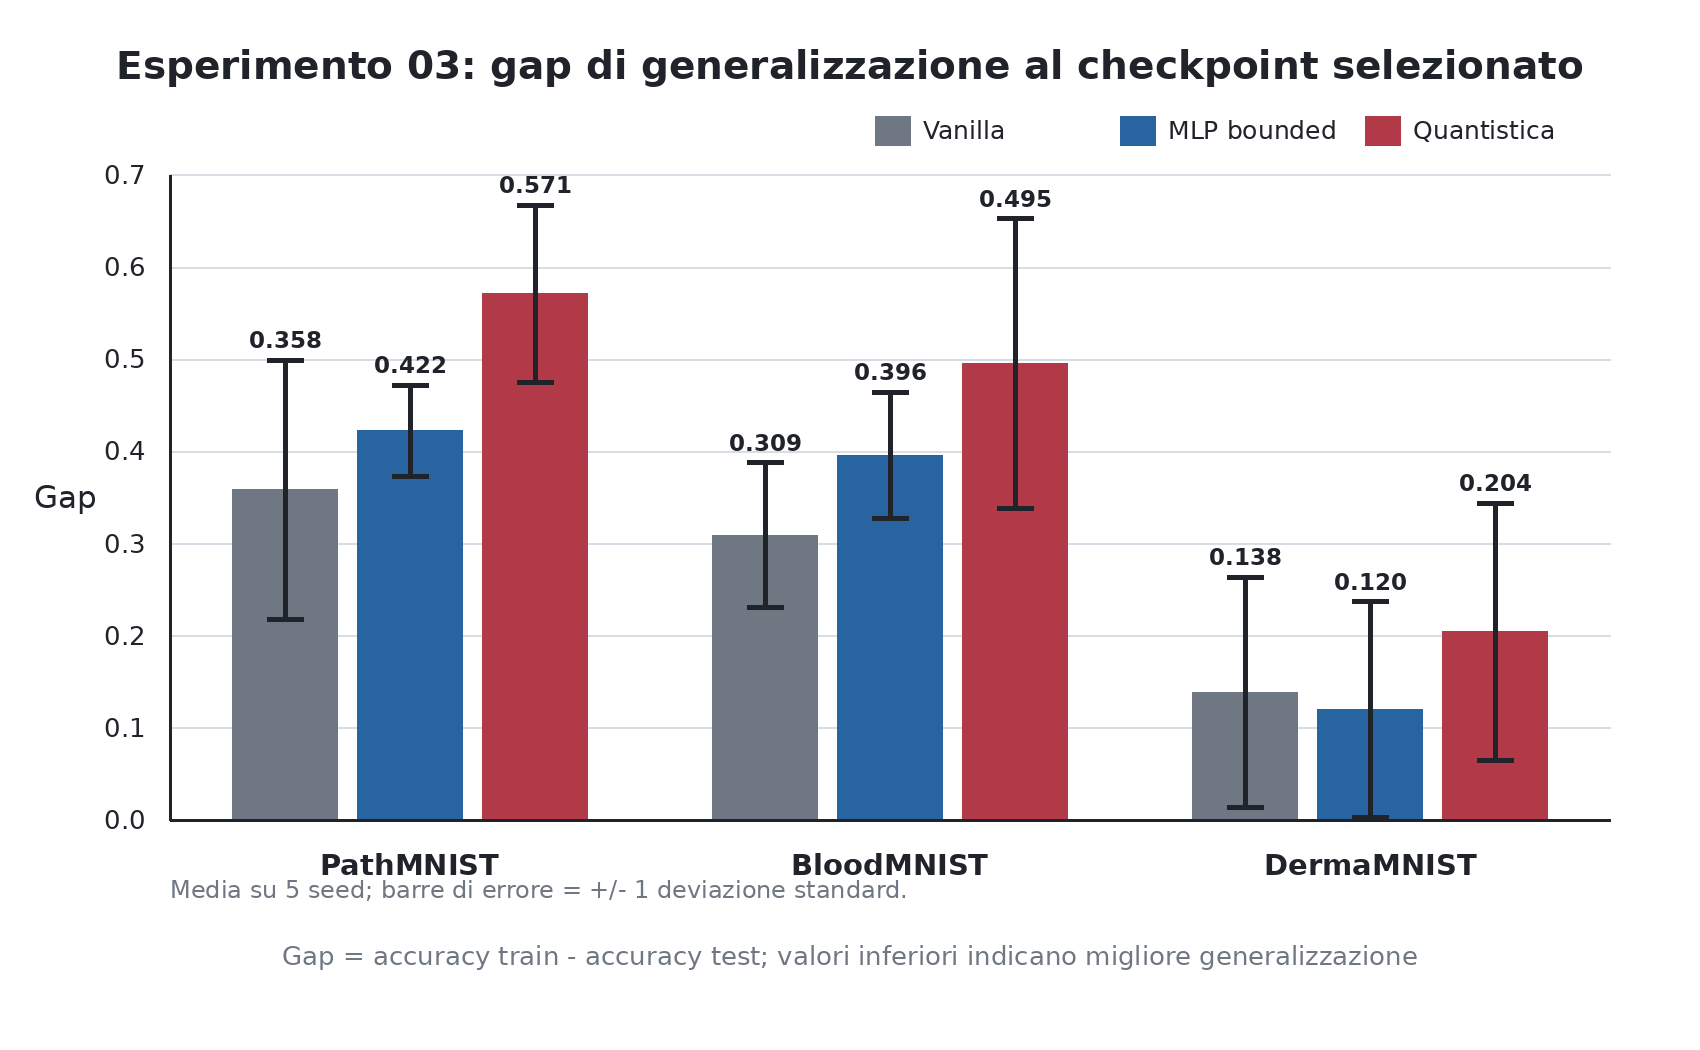
\includegraphics[width=.72\textwidth]{figure/experiment_03_gap_by_dataset.png}
\caption[Esperimento 03: gap per dataset]{Gap medio di generalizzazione nelle
tre varianti \code{vanilla}, \code{bounded\_mlp} e \code{quantum\_reg} (in figura
«Vanilla», «MLP bounded» e «Quantistica»); barre: una deviazione standard sui
seed.}
\label{fig:gap-03}
\end{figure}

\begin{figure}[htbp]
  \centering
  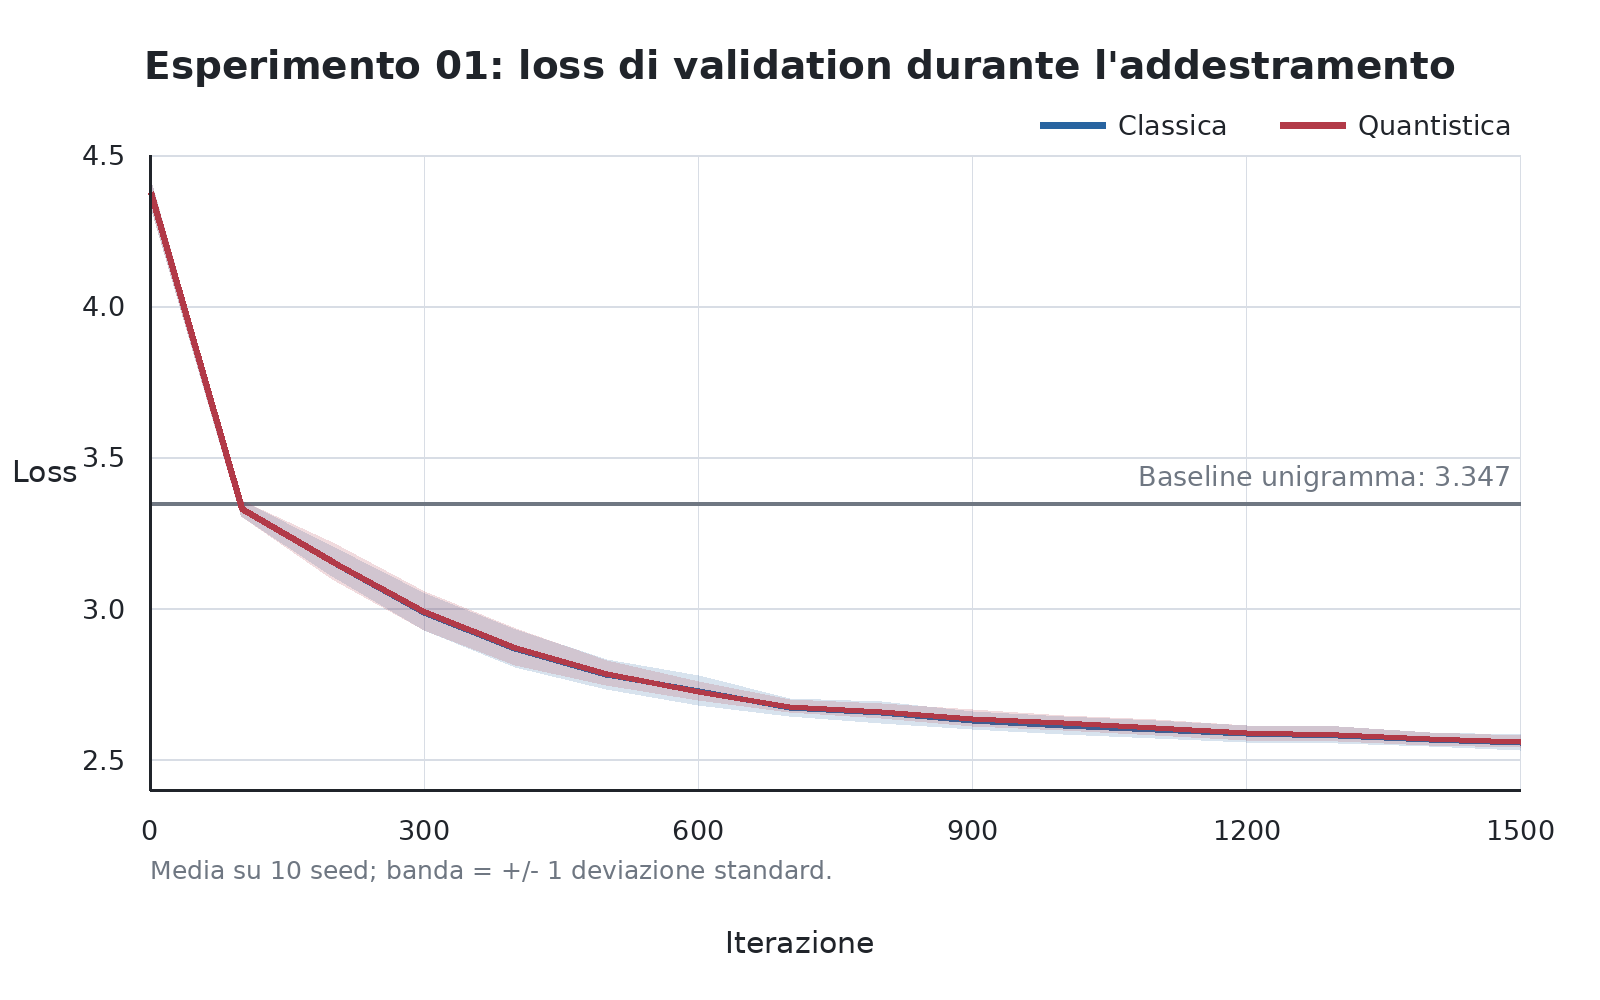
\includegraphics[width=.72\textwidth]{figure/experiment_01_learning_curves.png}
  \caption[Esperimento 01: curve di validation]{Loss di validation media sui
  dieci seed; la banda rappresenta una deviazione standard. La linea orizzontale
  è la baseline unigramma sullo split di validation. Le curve delle due varianti
  sono praticamente sovrapposte; il confronto quantitativo è nella
  \cref{fig:paired-01}.}
  \label{fig:curve-01}
\end{figure}

\begin{figure}[htbp]
\centering
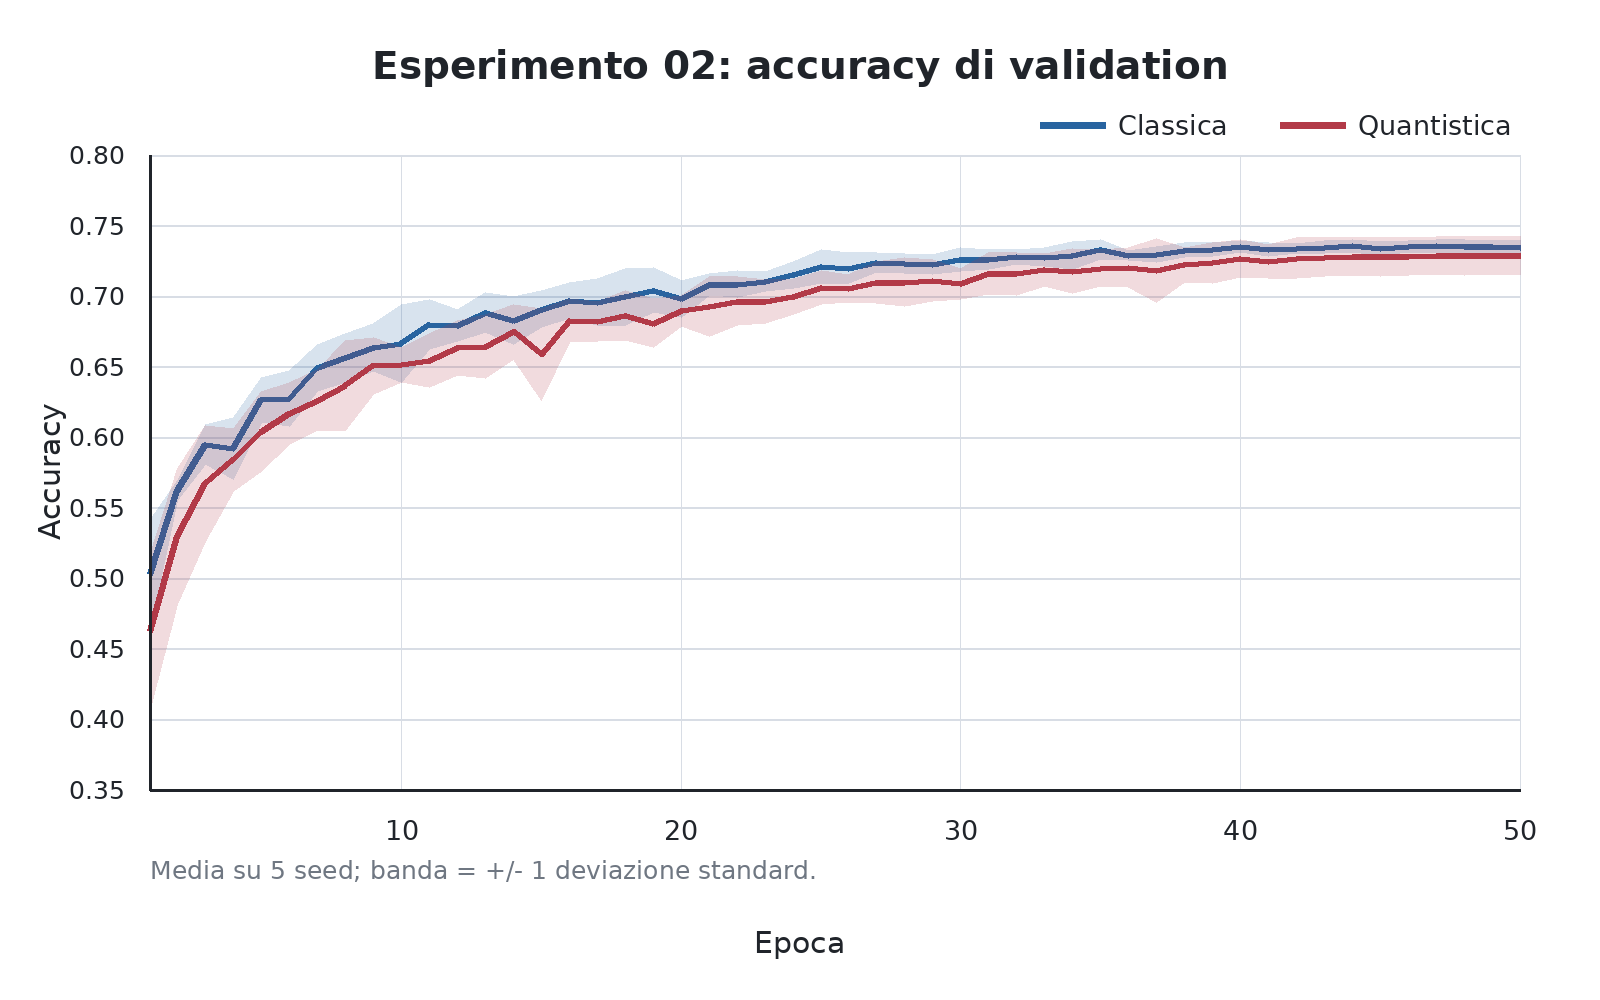
\includegraphics[width=.72\textwidth]{figure/experiment_02_learning_curves.png}
\caption[Esperimento 02: curve di validation]{Accuracy di validation media sui
cinque seed per le varianti classica e quantistica; la banda rappresenta una
deviazione standard.}
\label{fig:curve-02}
\end{figure}

\chapter{Dettagli circuitali}
\label{app:circuiti}

I diagrammi sono generati con \code{qml.draw} sui circuiti istanziati dal codice.

\section{Corrispondenza fra teoria e implementazione}

\begin{table}[htbp]
\centering
\caption[Corrispondenza fra formulazione teorica e implementazione]{%
Corrispondenza fra gli elementi teorici del \cref{cap:transformer} e le classi che
li implementano. Salvo diversa indicazione, il file è
\file{experiments/01\_quantum\_gpt/src/model.py}.}
\label{tab:corrispondenza-gpt}
\small
\begin{tabularx}{\textwidth}{@{}l l X@{}}
\toprule
\textbf{Elemento teorico} & \textbf{Classe / metodo} & \textbf{File} \\
\midrule
Embedding di token e posizione & \code{QuantumGPT.\_\_init\_\_} & \file{src/model.py} \\
Attenzione a testa singola & \classe{Head} & idem \\
Maschera causale & \code{Head.tril} (buffer) & idem \\
Attenzione multi-testa & \classe{MultiHeadAttention} & idem \\
Rete feed-forward & \classe{FeedForward} & idem \\
Blocco pre-norm & \classe{Block} & idem \\
Obiettivo autoregressivo & \code{QuantumGPT.forward} & idem \\
Generazione & \code{QuantumGPT.generate} & idem \\
Proiezione $Q,K,V$ quantistica & \classe{QuantumLayerAdapter} & \file{src/quantum\_layers.py} \\
\quad (alias di) & \classe{QuantumLinearWithAdapter} & \file{quantum\_linear.py} \\
\bottomrule
\end{tabularx}
\end{table}

\section{Circuito variazionale degli esperimenti 01--03}

Il circuito è \code{AngleEmbedding} seguito da \code{StronglyEntanglingLayers}
con $\nqlayers = 2$, con misura di $\expval{Z_i}$ su ogni qubit
(\cref{sec:quantum-linear}).

I tre casi differiscono per il numero di fili. Il comando seguente genera
diagramma e specifiche con la versione installata di PennyLane:

\begin{lstlisting}[style=python, numbers=none]
import pennylane as qml
from quantum_framework.layers import QuantumLinear

layer = QuantumLinear(n_qubits=10, n_qlayers=2)
print(qml.draw(layer.qlayer.qnode)(inputs, weights))
print(qml.specs(layer.qlayer.qnode)(inputs, weights))
\end{lstlisting}

\section{Circuito di kernel IQP dell'esperimento 04}

Il circuito \code{kernel\_circuit} realizza
$K(x,y) = \abs{\bra{0}\Uenc^{\dagger}(y)\Uenc(x)\ket{0}}^2$ dell'
\cref{eq:fidelity-kernel} con $\nq = 8$.

Il calcolo applica prima $\Uenc(x)$ e poi $\Uenc^{\dagger}(y)$; la probabilità
di ritrovare $\ket{0}^{\otimes8}$ è la fedeltà. Il controllo a vettore di stato
costruisce esplicitamente i due stati.

\section{Dimensioni dei circuiti}

\begin{center}
\begin{tabular}{@{}l r r r@{}}\toprule
\textbf{Esperimento}&\textbf{Qubit}&\textbf{Pesi VQC}&\textbf{Ampiezze}\\\midrule
01&4&24 per circuito&16\\
02&8&48&256\\
03&10&60&1024\\
04&8&0 addestrabili&256\\\bottomrule
\end{tabular}
\end{center}
Per 01 il modello contiene più istanze del circuito nelle proiezioni $Q,K,V$;
il valore in tabella è riferito a una singola istanza.

% ===========================================================================
%  Appendice E — Inventario delle run
% ===========================================================================
\chapter{Inventario delle run}
\label{app:inventario}

Questa appendice elenca ogni esecuzione utilizzata nella tesi. Serve a rendere
verificabile l'affermazione, posta nella \cref{sec:minacce}, che nessuna run
storica a schema diverso sia stata mescolata alle run della campagna definitiva.

\begin{center}\small
\begin{tabular}{@{}l l l l@{}}\toprule
\textbf{Esp.}&\textbf{Unità appaiate}&\textbf{Artefatto canonico}&\textbf{Stato}\\\midrule
01&10 seed, 20 run&\code{experiment\_01\_quantum\_gpt\_n10.json}&completo\\
02&5 seed, 10 run&\code{experiment\_02\_quantum\_vit\_n5.json}&completo\\
03&3 dataset, 5 seed, 45 run&\code{experiment\_03\_quantum\_reg\_n100\_steps400.json}&completo\\
04&20 sottocampioni&\code{experiment\_04\_quantum\_kernel\_frozen.json}&completo\\\bottomrule
\end{tabular}\end{center}

Gli artefatti sono in \file{docs/checkpoints}; l'elenco degli hash SHA-256 è
in \file{docs/HANDOFF.md}. I manifest originali registrano il commit
\code{b91c318ce87e697d7da459cd209a4c11a742fb11} e \code{dirty=true}. I percorsi
delle singole run, seed, tempi, configurazioni e versioni di schema sono
preservati negli aggregati, evitando una seconda trascrizione manuale.

\section{Run storiche}

\begin{limite}
Le run precedenti all'unificazione dello schema vanno marcate esplicitamente in
questa tabella e nelle sezioni in cui compaiono. In particolare: le run
dell'esperimento~02 anteriori alla campagna definitiva non sono appaiate (dataset
diversi fra la variante classica e quella quantistica) e usano uno schema privo
dei campi \code{test\_accuracy} e \code{dataset}; non sostengono alcuna
conclusione principale.
\end{limite}


% ----------------------------------------------------------- BIBLIOGRAFIA ---
\backmatter
\printbibliography[heading=bibintoc, title={Bibliografia}]

\end{document}
